\documentclass[]{book}
\usepackage{lmodern}
\usepackage{amssymb,amsmath}
\usepackage{ifxetex,ifluatex}
\usepackage{fixltx2e} % provides \textsubscript
\ifnum 0\ifxetex 1\fi\ifluatex 1\fi=0 % if pdftex
  \usepackage[T1]{fontenc}
  \usepackage[utf8]{inputenc}
\else % if luatex or xelatex
  \ifxetex
    \usepackage{mathspec}
  \else
    \usepackage{fontspec}
  \fi
  \defaultfontfeatures{Ligatures=TeX,Scale=MatchLowercase}
\fi
% use upquote if available, for straight quotes in verbatim environments
\IfFileExists{upquote.sty}{\usepackage{upquote}}{}
% use microtype if available
\IfFileExists{microtype.sty}{%
\usepackage{microtype}
\UseMicrotypeSet[protrusion]{basicmath} % disable protrusion for tt fonts
}{}
\usepackage[margin=1in]{geometry}
\usepackage{hyperref}
\hypersetup{unicode=true,
            pdftitle={MATH2011: Statistical Distribution Theory},
            pdfauthor={Dr Helen Ogden},
            pdfborder={0 0 0},
            breaklinks=true}
\urlstyle{same}  % don't use monospace font for urls
\usepackage{natbib}
\bibliographystyle{plainnat}
\usepackage{color}
\usepackage{fancyvrb}
\newcommand{\VerbBar}{|}
\newcommand{\VERB}{\Verb[commandchars=\\\{\}]}
\DefineVerbatimEnvironment{Highlighting}{Verbatim}{commandchars=\\\{\}}
% Add ',fontsize=\small' for more characters per line
\usepackage{framed}
\definecolor{shadecolor}{RGB}{248,248,248}
\newenvironment{Shaded}{\begin{snugshade}}{\end{snugshade}}
\newcommand{\KeywordTok}[1]{\textcolor[rgb]{0.13,0.29,0.53}{\textbf{#1}}}
\newcommand{\DataTypeTok}[1]{\textcolor[rgb]{0.13,0.29,0.53}{#1}}
\newcommand{\DecValTok}[1]{\textcolor[rgb]{0.00,0.00,0.81}{#1}}
\newcommand{\BaseNTok}[1]{\textcolor[rgb]{0.00,0.00,0.81}{#1}}
\newcommand{\FloatTok}[1]{\textcolor[rgb]{0.00,0.00,0.81}{#1}}
\newcommand{\ConstantTok}[1]{\textcolor[rgb]{0.00,0.00,0.00}{#1}}
\newcommand{\CharTok}[1]{\textcolor[rgb]{0.31,0.60,0.02}{#1}}
\newcommand{\SpecialCharTok}[1]{\textcolor[rgb]{0.00,0.00,0.00}{#1}}
\newcommand{\StringTok}[1]{\textcolor[rgb]{0.31,0.60,0.02}{#1}}
\newcommand{\VerbatimStringTok}[1]{\textcolor[rgb]{0.31,0.60,0.02}{#1}}
\newcommand{\SpecialStringTok}[1]{\textcolor[rgb]{0.31,0.60,0.02}{#1}}
\newcommand{\ImportTok}[1]{#1}
\newcommand{\CommentTok}[1]{\textcolor[rgb]{0.56,0.35,0.01}{\textit{#1}}}
\newcommand{\DocumentationTok}[1]{\textcolor[rgb]{0.56,0.35,0.01}{\textbf{\textit{#1}}}}
\newcommand{\AnnotationTok}[1]{\textcolor[rgb]{0.56,0.35,0.01}{\textbf{\textit{#1}}}}
\newcommand{\CommentVarTok}[1]{\textcolor[rgb]{0.56,0.35,0.01}{\textbf{\textit{#1}}}}
\newcommand{\OtherTok}[1]{\textcolor[rgb]{0.56,0.35,0.01}{#1}}
\newcommand{\FunctionTok}[1]{\textcolor[rgb]{0.00,0.00,0.00}{#1}}
\newcommand{\VariableTok}[1]{\textcolor[rgb]{0.00,0.00,0.00}{#1}}
\newcommand{\ControlFlowTok}[1]{\textcolor[rgb]{0.13,0.29,0.53}{\textbf{#1}}}
\newcommand{\OperatorTok}[1]{\textcolor[rgb]{0.81,0.36,0.00}{\textbf{#1}}}
\newcommand{\BuiltInTok}[1]{#1}
\newcommand{\ExtensionTok}[1]{#1}
\newcommand{\PreprocessorTok}[1]{\textcolor[rgb]{0.56,0.35,0.01}{\textit{#1}}}
\newcommand{\AttributeTok}[1]{\textcolor[rgb]{0.77,0.63,0.00}{#1}}
\newcommand{\RegionMarkerTok}[1]{#1}
\newcommand{\InformationTok}[1]{\textcolor[rgb]{0.56,0.35,0.01}{\textbf{\textit{#1}}}}
\newcommand{\WarningTok}[1]{\textcolor[rgb]{0.56,0.35,0.01}{\textbf{\textit{#1}}}}
\newcommand{\AlertTok}[1]{\textcolor[rgb]{0.94,0.16,0.16}{#1}}
\newcommand{\ErrorTok}[1]{\textcolor[rgb]{0.64,0.00,0.00}{\textbf{#1}}}
\newcommand{\NormalTok}[1]{#1}
\usepackage{longtable,booktabs}
\usepackage{graphicx,grffile}
\makeatletter
\def\maxwidth{\ifdim\Gin@nat@width>\linewidth\linewidth\else\Gin@nat@width\fi}
\def\maxheight{\ifdim\Gin@nat@height>\textheight\textheight\else\Gin@nat@height\fi}
\makeatother
% Scale images if necessary, so that they will not overflow the page
% margins by default, and it is still possible to overwrite the defaults
% using explicit options in \includegraphics[width, height, ...]{}
\setkeys{Gin}{width=\maxwidth,height=\maxheight,keepaspectratio}
\IfFileExists{parskip.sty}{%
\usepackage{parskip}
}{% else
\setlength{\parindent}{0pt}
\setlength{\parskip}{6pt plus 2pt minus 1pt}
}
\setlength{\emergencystretch}{3em}  % prevent overfull lines
\providecommand{\tightlist}{%
  \setlength{\itemsep}{0pt}\setlength{\parskip}{0pt}}
\setcounter{secnumdepth}{5}
% Redefines (sub)paragraphs to behave more like sections
\ifx\paragraph\undefined\else
\let\oldparagraph\paragraph
\renewcommand{\paragraph}[1]{\oldparagraph{#1}\mbox{}}
\fi
\ifx\subparagraph\undefined\else
\let\oldsubparagraph\subparagraph
\renewcommand{\subparagraph}[1]{\oldsubparagraph{#1}\mbox{}}
\fi

%%% Use protect on footnotes to avoid problems with footnotes in titles
\let\rmarkdownfootnote\footnote%
\def\footnote{\protect\rmarkdownfootnote}

%%% Change title format to be more compact
\usepackage{titling}

% Create subtitle command for use in maketitle
\providecommand{\subtitle}[1]{
  \posttitle{
    \begin{center}\large#1\end{center}
    }
}

\setlength{\droptitle}{-2em}

  \title{MATH2011: Statistical Distribution Theory}
    \pretitle{\vspace{\droptitle}\centering\huge}
  \posttitle{\par}
    \author{Dr Helen Ogden}
    \preauthor{\centering\large\emph}
  \postauthor{\par}
      \predate{\centering\large\emph}
  \postdate{\par}
    \date{2019/20}

\usepackage{booktabs}
\usepackage{amsthm}
\usepackage{bm}
\makeatletter
\def\thm@space@setup{%
  \thm@preskip=8pt plus 2pt minus 4pt
  \thm@postskip=\thm@preskip
}
\makeatother

\usepackage{amsthm}
\newtheorem{theorem}{Theorem}[chapter]
\newtheorem{lemma}{Lemma}[chapter]
\newtheorem{corollary}{Corollary}[chapter]
\newtheorem{proposition}{Proposition}[chapter]
\newtheorem{conjecture}{Conjecture}[chapter]
\theoremstyle{definition}
\newtheorem{definition}{Definition}[chapter]
\theoremstyle{definition}
\newtheorem{example}{Example}[chapter]
\theoremstyle{definition}
\newtheorem{exercise}{Exercise}[chapter]
\theoremstyle{remark}
\newtheorem*{remark}{Remark}
\newtheorem*{solution}{Solution}
\let\BeginKnitrBlock\begin \let\EndKnitrBlock\end
\begin{document}
\maketitle

{
\setcounter{tocdepth}{1}
\tableofcontents
}
\part{Distributions and their
properties}\label{part-distributions-and-their-properties}

\chapter{Probability distributions}\label{probability-distributions}

\section{Random variables}\label{random-variables}

A random variable \(Y\) is described by its domain (or sample space)
\(D\) together with the probabilities assigned to subsets of the domain.
These define the \emph{probability distribution} of the random variable.
We distinguish between discrete and continuous random variables.

\textbf{Discrete} probability distributions are defined by a probability
(mass) function \[p(y)\equiv P(Y=y), \quad \text{for $y \in D$}\] where
\[\sum_{y\in D} p(y) =1.\] The distribution function \(F(\cdot)\) is
defined for all \(y \in \mathbb{R}\) by
\[F(y)\equiv P(Y \leq y) = \sum_{x\in D: \, x\leq y} p(x).\]

\textbf{Continuous} probability distributions are defined by a
probability density function (pdf) \(f(\cdot)\) where
\[P(y_1< Y \leq y_2) = \int_{y_1}^{y_2} f(y) dy.\] The domain of \(Y\)
is the set \(D = \{y \in \mathbb{R}: f(y) > 0\}\) Hence
\[\int_{-\infty}^\infty f(y) dy = \int_D f(y) dy = 1.\] The distribution
function \(F(\cdot)\) is then given by
\[F(y)\equiv P(Y \leq y) = \int_{-\infty}^y f(x) dx.\] Therefore
\[P(y_1< Y \leq y_2) = F(y_2) - F(y_1)\] and
\[f(y) = \frac{d}{dy} F(y).\]

\section{Examples of discrete
distributions}\label{examples-of-discrete-distributions}

\subsection{The Bernoulli
distribution}\label{the-bernoulli-distribution}

A \emph{Bernoulli trial} is an experiment with just two possible
outcomes `success' and `failure' which occur with probabilities
\(\theta\) and \(1- \theta\) respectively, where \(\theta\) is the
success probability. The indicator of success in a Bernoulli trial has
Bernoulli distribution.

\BeginKnitrBlock{definition}
\protect\hypertarget{def:unnamed-chunk-1}{}{\label{def:unnamed-chunk-1} }A
discrete random variables \(Y\) has \emph{Bernoulli} distribution if it
has probability function of the form
\[p(y) = \theta^y (1- \theta)^{1-y}, \quad y = 0, 1,\] for some
\(0 < \theta < 1\). We write \(Y \sim \text{Bernoulli}(\theta)\).
\EndKnitrBlock{definition}

\subsection{The binomial distribution}\label{the-binomial-distribution}

Suppose we undertake a fixed number, \(n\), of independent Bernoulli
trials, each with success probability \(\theta\). Let \(Y\) be the
number of successes in these \(n\) trials. Then \(Y\) has
\emph{binomial} distribution.

\BeginKnitrBlock{definition}
\protect\hypertarget{def:unnamed-chunk-2}{}{\label{def:unnamed-chunk-2} }A
discrete random variables \(Y\) has \emph{binomial} distribution if it
has probability function of the form
\[p(y) = \binom{n}{y} \theta^x (1 - \theta)^{n-y}, \quad y = 0, 1, \ldots, n,\]
for some \(n \in \mathbb{N}\) and \(0 < \theta < 1\). We write
\(Y \sim \text{binomial}(n, \theta)\).
\EndKnitrBlock{definition}

\subsection{The negative binomial
distribution}\label{the-negative-binomial-distribution}

Suppose we undertake a sequence of independent Bernoulli trials, each
with success probability \(\theta\). Let \(X\) be the number failures
that occur before the \(k\)th success. Then \(X\) has \emph{negative
binomial} distribution. \BeginKnitrBlock{definition}

\protect\hypertarget{def:unnamed-chunk-3}{}{\label{def:unnamed-chunk-3} }A
discrete random variables \(Y\) has \emph{negative binomial}
distribution if it has probability function of the form
\[p(y) = \binom{k + y - 1}{y} (1 - \theta)^y \theta^k, \quad
  y = 0, 1, \ldots,
\] for some \(k \in \mathbb{N}\), and \(0 < \theta < 1\). We write
\(Y \sim \text{negbin}(k, \theta)\).
\EndKnitrBlock{definition}

The \emph{geometric} distribution is the special case of the negative
binomial distribution with \(k = 1\): the number of failures that occur
before the first success.

\BeginKnitrBlock{definition}
\protect\hypertarget{def:unnamed-chunk-4}{}{\label{def:unnamed-chunk-4} }A
discrete random variables \(Y\) has \emph{geometric} distribution if it
has probability function of the form
\[p(y) = (1 - \theta)^y \theta, \quad
  y = 0, 1, \ldots,
\] for some \(0 < \theta < 1\). We write
\(Y \sim \text{geometric}(\theta)\).
\EndKnitrBlock{definition}

\subsection{The Poisson distribution}\label{poisson}

The \emph{Poisson} distribution arises in a variety of practical
situations where we are interested in modelling counts of how often an
`event' occurs.

\BeginKnitrBlock{definition}
\protect\hypertarget{def:unnamed-chunk-5}{}{\label{def:unnamed-chunk-5} }A
discrete random variable \(Y\) has \emph{Poisson} distribution if it has
probability function of the form
\[p(y) = \frac{e^{-\theta} (\theta)^y}{y!}, \quad y = 0, 1, \ldots,\]
for some \emph{rate parameter} \(\theta > 0\). We write
\(Y \sim \text{Poisson}(\theta)\).
\EndKnitrBlock{definition}

In a \emph{Poisson process}, events occur at random at constant rate
\(\theta\) per unit time, independent of all other events. If we define
\(Y\) as the number of events of a Poisson process in an interval of
fixed length \(t\), then \(Y \sim \text{Poisson}(t \theta)\).

\section{Examples of continuous
distributions}\label{examples-of-continuous-distributions}

\subsection{The exponential
distribution}\label{the-exponential-distribution}

In Section \ref{poisson}, we considered the Poisson process, in which
events occur at random, at a rate \(\theta\) per unit time. The actual
number of events which take place in any given unit of time has
\(\text{Poisson}(\theta)\) distribution. The \emph{exponential}
distribution represents the time between consecutive events in this
process.

Let \(Y\) represent the time interval between two events. Clearly this
variable cannot be negative, but can take any positive value. The domain
of \(Y\) is \((0, \infty)\). We have

\begin{align*}
P(Y > y) &= P(\text{no events in an interval of length $y$}) \\
&= \frac{e^{-\theta y} (\theta y)^0}{0!} \\
&= e^{-\theta y}
\end{align*}

so \[F(y) = P(Y \leq y) = 1 - e^{-\theta y}, \quad y > 0.\]
Differentiating, we obtain the pdf
\[f(y) = \frac{d}{dy} F(y) = \theta e^{-\theta y}, \quad y > 0.\]

\BeginKnitrBlock{definition}
\protect\hypertarget{def:unnamed-chunk-6}{}{\label{def:unnamed-chunk-6} }A
random variable \(Y\) has \emph{exponential} distribution if it has pdf
of the form \[f(y) = \theta e^{-\theta y}, \quad y > 0,\] for some
\emph{rate parameter} \(\theta > 0\). We write
\(Y \sim \text{exponential}(\theta)\).
\EndKnitrBlock{definition}

\BeginKnitrBlock{example}
\protect\hypertarget{exm:unnamed-chunk-7}{}{\label{exm:unnamed-chunk-7} }
Suppose the lifetime in hours of a certain type of electronic component
is described by an Exponential random variable with rate parameter
\(\theta = 0.01\). What is the probability such a component will have a
lifetime of between \(100\) and \(200\) hours?

The probability is the area under the curve \(f(y) = 0.01 e^{-0.01 y}\)
between \(y = 100\) and \(y = 200\), so

\begin{align*}
P(100 < Y \leq 200) &= \int_{100}^{200} 0.01e^{-0.01 y} dy \\
&= e^{-1} - e^{-2} = 0.37 - 0.14 = 0.23.
\end{align*}
\EndKnitrBlock{example} We could find this in \texttt{R} with

\begin{Shaded}
\begin{Highlighting}[]
\KeywordTok{pexp}\NormalTok{(}\DecValTok{200}\NormalTok{, }\DataTypeTok{rate =} \FloatTok{0.01}\NormalTok{) }\OperatorTok{-}\StringTok{ }\KeywordTok{pexp}\NormalTok{(}\DecValTok{100}\NormalTok{, }\DataTypeTok{rate =} \FloatTok{0.01}\NormalTok{)}
\end{Highlighting}
\end{Shaded}

\begin{verbatim}
## [1] 0.2325442
\end{verbatim}

\subsection{The uniform distribution}\label{the-uniform-distribution}

The uniform distribution is one of the simplest probability
distributions: it just places a constant density between some range
\((a, b)\):

\BeginKnitrBlock{definition}
\protect\hypertarget{def:unnamed-chunk-9}{}{\label{def:unnamed-chunk-9} }A
random variable \(Y\) has \emph{uniform} distribution if it has pdf of
the form \[f(y) = \frac{1}{b-a}, a < y < b,\] for some parameters
\(a, b \in \mathbb{R}\), with \(b > a\). We write \(Y \sim U(a, b)\).
\EndKnitrBlock{definition}

\subsection{The normal distribution}\label{the-normal-distribution}

The normal distribution is probably the single most important
distribution in statistics. The main reason for its importance is the
central limit theorem, which you have seen before in MATH1024, and which
we will prove in Section \ref{clt}.

\BeginKnitrBlock{definition}
\protect\hypertarget{def:unnamed-chunk-10}{}{\label{def:unnamed-chunk-10} }A
random variable \(Y\) has \emph{normal} distribution if it has pdf of
the form \[f(y) = \frac{1}{\sqrt{2 \pi \sigma^2}}
\exp\left\{-\frac{1}{2 \sigma^2} (y - \mu)^2 \right\},\] for some
parameters \(\mu \in \mathbb{R}\) and \(\sigma^2 > 0\). We write
\(Y \sim N(\mu, \sigma^2)\).
\EndKnitrBlock{definition}

\BeginKnitrBlock{example}
\protect\hypertarget{exm:unnamed-chunk-11}{}{\label{exm:unnamed-chunk-11}
}Suppose that daily water use at a factory varies about a mean of
\(77500\) litres with standard deviation \(5700\) litres. If demand is
normally distributed

\begin{enumerate}
\def\labelenumi{\arabic{enumi}.}
\tightlist
\item
  What proportion of days does the demand fall short of \(70000\)
  litres?
\item
  What proportion of days does demand exceed \(90000\) litres?
\item
  What is your reaction to a demand of \(175000\) gallons?
\end{enumerate}

Writing \(X\) for the daily water use in litres , we have
\(X \sim N(77500, 5700^2)\) We can use \texttt{R} to compute the
probability \(P(X < 70000) = F(70000)\)
\EndKnitrBlock{example}

\begin{Shaded}
\begin{Highlighting}[]
\KeywordTok{pnorm}\NormalTok{(}\DecValTok{70000}\NormalTok{, }\DataTypeTok{mean =} \DecValTok{77500}\NormalTok{, }\DataTypeTok{sd =} \DecValTok{5700}\NormalTok{)}
\end{Highlighting}
\end{Shaded}

\begin{verbatim}
## [1] 0.09412236
\end{verbatim}

so the daily water use will be less than \(70000\) litres about
\(9.4\%\) of the time.

We can find \(P(x > 90000) = 1 - F(90000)\)

\begin{Shaded}
\begin{Highlighting}[]
\DecValTok{1} \OperatorTok{-}\StringTok{ }\KeywordTok{pnorm}\NormalTok{(}\DecValTok{90000}\NormalTok{, }\DataTypeTok{mean =} \DecValTok{77500}\NormalTok{, }\DataTypeTok{sd =} \DecValTok{5700}\NormalTok{)}
\end{Highlighting}
\end{Shaded}

\begin{verbatim}
## [1] 0.01415432
\end{verbatim}

so the daily water use will be more than \(90000\) litres about
\(1.4\%\) of the time.

We can find \(P(x > 175000) = 1 - F(175000)\)

\begin{Shaded}
\begin{Highlighting}[]
\DecValTok{1} \OperatorTok{-}\StringTok{ }\KeywordTok{pnorm}\NormalTok{(}\DecValTok{175000}\NormalTok{, }\DataTypeTok{mean =} \DecValTok{77500}\NormalTok{, }\DataTypeTok{sd =} \DecValTok{5700}\NormalTok{)}
\end{Highlighting}
\end{Shaded}

\begin{verbatim}
## [1] 0
\end{verbatim}

In fact, the number is not exactly zero, but it is so small that the
computer is rounding it to zero. Such an extreme water use is therefore
surprising, and an explanation should be sought. It is possible that a
error has occurred in recording the water use, such as two days data
being taken together. Alternatively, perhaps our model which assumes
that \(X \sim N(77500, 5700^2)\) is incorrect. This idea of surprise at
an extreme result of low probability, as predicted by a statistical
model, will be important later in this module and also in modules such
as MATH2010 Statistical Modelling I.

\chapter{Moments}\label{moments}

\section{Expected value}\label{expected-value}

Suppose we have a discrete random variable \(Y\) with probability
function \(p(.)\) with domain \(D\). Although \(p(.)\) tells us
everything about the properties of \(Y\), it is often useful to
summarise the properties \(Y\) using a few simple quantities.

A simple summary of the probabilistic properties of \(Y\) is the
\emph{expected value} or (population) \emph{mean} of \(Y\), denoted by
\(E(Y)\) or \(\mu\), depending on the context.

\BeginKnitrBlock{definition}
\protect\hypertarget{def:unnamed-chunk-15}{}{\label{def:unnamed-chunk-15}
}If \(Y\) is a discrete random variable with probability function
\(p(.)\) and domain \(D\), the expected value of \(Y\) is
\[\mu = E(Y) = \sum_{y \in D} y p(y).\] If \(Y\) is a continuous random
variable with probability density function \(f(.)\) and domain \(D\),
the expected value of Y is:
\[\mu = E(Y) = \int_{-\infty}^\infty y f(y)dy = \int_D y f(y) dy.\]
\EndKnitrBlock{definition}

\BeginKnitrBlock{example}[Expected value of the Bernoulli distribution]
\protect\hypertarget{exm:bernoullimean}{}{\label{exm:bernoullimean}
\iffalse (Expected value of the Bernoulli distribution) \fi{} }Suppose
\(Y \sim \text{Bernoulli}(\theta)\). Then
\[E(Y) = \sum_{y \in \{0, 1\}} y p(y) = 0 \times (1- \theta) + 1 \times \theta = \theta.\]
\EndKnitrBlock{example}

\BeginKnitrBlock{example}[Expected value of the exponential distribution]
\protect\hypertarget{exm:expmean}{}{\label{exm:expmean} \iffalse (Expected
value of the exponential distribution) \fi{} }Suppose
\(Y \sim \text{exponential}(\theta)\). Then

\begin{align*}
E(Y) &= \int_{0}^\infty y \theta e^{-\theta y} dy  \\
&= \frac{1}{\theta} \int_{0}^\infty t e^{-t} dt \\
&= \frac{1}{\theta} \left\{[-t e^{-t}]_0^\infty + \int_0^\infty e^{-t}dt \right\} \\
&= \frac{1}{\theta} \{0 + 1\} = \frac{1}{\theta}.
\end{align*}

Note that we have shown \(\int_{0}^\infty t e^{-t} dt = 1\): this result
will be useful later on.
\EndKnitrBlock{example}

We can find the expected value of new random variable \(h(Y)\) with
\[E[h(Y)] = \int_{-\infty}^{\infty} h(y) f(y) dy = \int_D h(y) f(y) dy\]
if \(Y\) is a continuous random variable with pdf \(f(.)\). We may
obtain a similar expression in the discrete case.

\section{Variance}\label{variance}

\BeginKnitrBlock{definition}
\protect\hypertarget{def:unnamed-chunk-16}{}{\label{def:unnamed-chunk-16}
}The (population) variance of \(Y\) is
\[ \text{Var}(Y) = E\left\{[Y - E(Y)]^2 \right\}.\]
\EndKnitrBlock{definition}

It is easy to show that \[ \text{Var}(Y) = E(Y^2) - [E(Y)]^2.\]
\(\text{Var}(Y)\) is a measure of spread, and is often denoted by
\(\sigma^2\).

We sometimes use the (population) standard deviation, which is just the
square root of the variance, to return to the original scale of
measurement of \(Y\).

\BeginKnitrBlock{example}[Variance of the Bernoulli distribution]
\protect\hypertarget{exm:unnamed-chunk-17}{}{\label{exm:unnamed-chunk-17}
\iffalse (Variance of the Bernoulli distribution) \fi{} }Suppose
\(Y \sim \text{Bernoulli}(\theta)\). We have seen in Example
\ref{exm:bernoullimean} that \(E(Y) = \theta\). We have
\[E(Y^2) = \sum_{y \in \{0, 1\}} y^2 p(y) = 0^2 \times (1- \theta) + 1^2 \times \theta
= \theta,\] so
\[\text{Var}(Y) = E(Y^2) - [E(Y)]^2 = \theta - \theta^2 = \theta ( 1 - \theta).\]
\EndKnitrBlock{example}

\BeginKnitrBlock{example}[Variance of the exponential distribution]
\protect\hypertarget{exm:expvar}{}{\label{exm:expvar} \iffalse (Variance of
the exponential distribution) \fi{} }Suppose
\(Y \sim \text{exponential}(\theta)\). We have seen in Example
\ref{exm:expmean} that \(E(Y) = 1/\theta\). We have

\begin{align*}
E(Y^2) &= \int_{0}^\infty y^2 \theta e^{-\theta y} dy  \\
&= \frac{1}{\theta^2} \int_{0}^\infty t^2 e^{-t} dt \\
&= \frac{1}{\theta} \left\{[-t^2 e^{-t}]_0^\infty + 2 \int_0^\infty t e^{-t}dt \right\} \\
&= \frac{1}{\theta^2} \{0 + 2\} = \frac{2}{\theta^2},
\end{align*}

since we saw in Example \ref{exm:expmean} that
\(\int_0^\infty t e^{-t}dt = 1\). So
\[\text{Var}(Y) = E(Y^2) - [E(Y)]^2 = \frac{2}{\theta^2} - \frac{1}{\theta^2} 
= \frac{1}{\theta^2}.\]
\EndKnitrBlock{example}

\section{Higher-order moments}\label{higher-order-moments}

So far we have summarised random variables using the mean and variance
(or standard deviation), which measure the ``location'' and the
``spread''. Why would we need anything more? Consider the following two
density functions of two different continuous distributions:

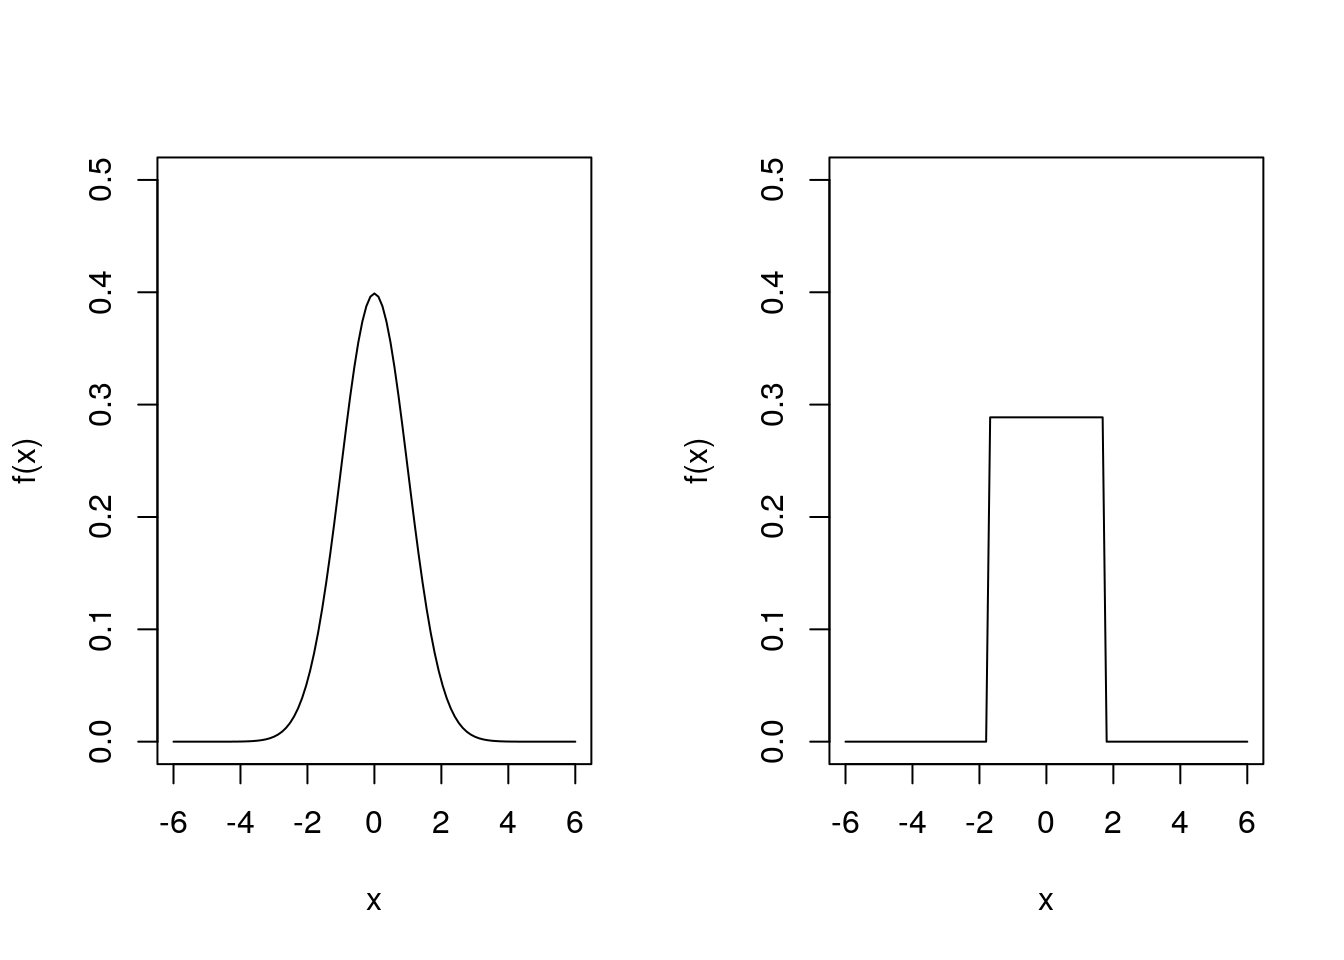
\includegraphics{MATH2011_files/figure-latex/unnamed-chunk-18-1.pdf}

In fact, the plot on the left is the pdf of a \(N(0, 1)\) distribution,
and the plot on the right is the pdf of a
\(\text{Uniform}(-\sqrt{3}, \sqrt{3})\) distribution. Both have mean
\(0\) and variance \(1\), yet they look very different. They are both
symmetric about \(0\) (the mean) but differ in terms of ``shape''.

Consider two more density functions:

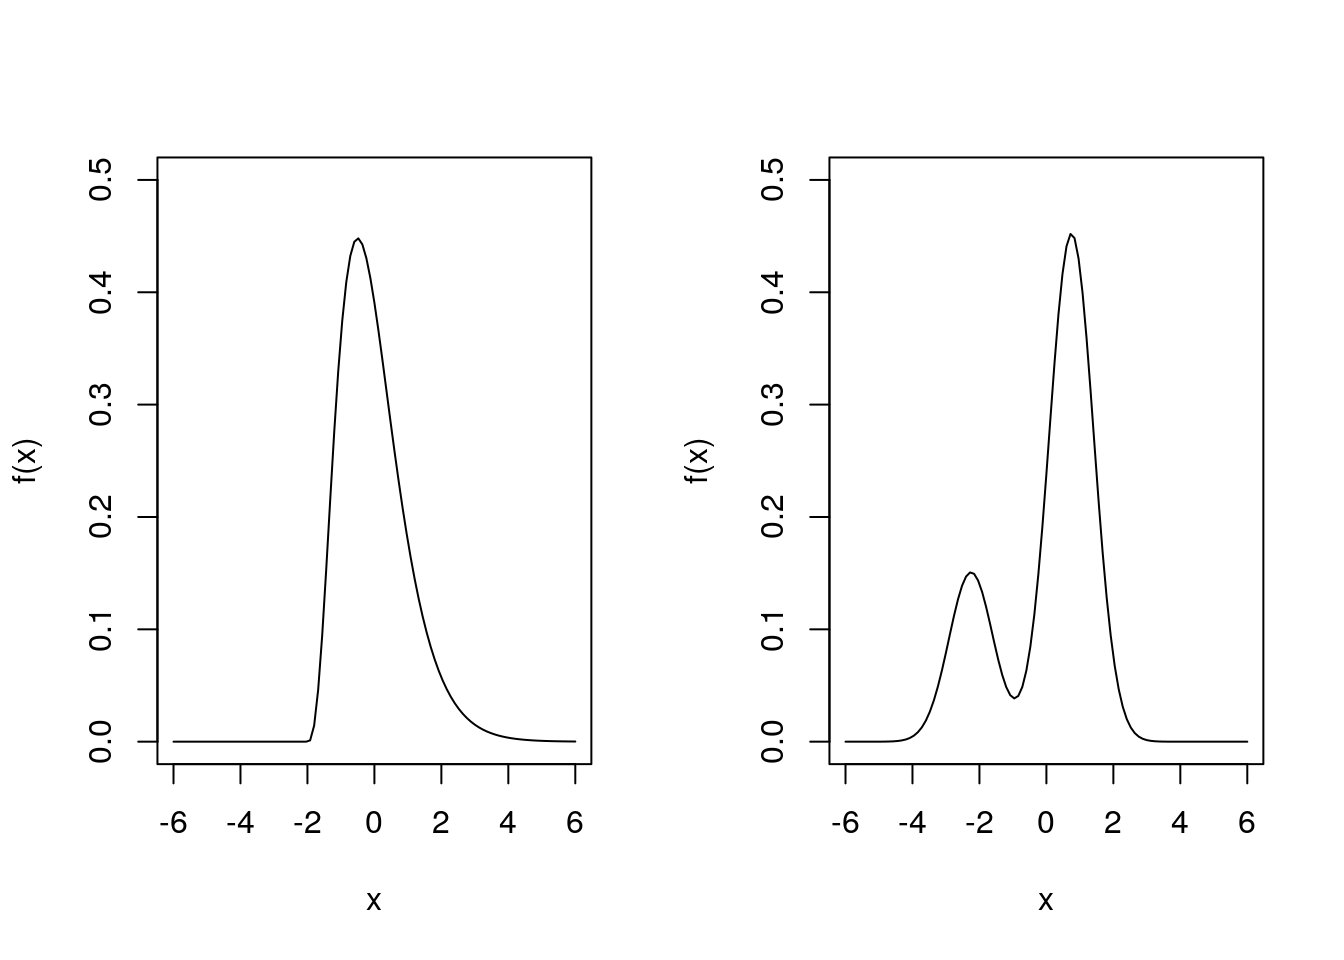
\includegraphics{MATH2011_files/figure-latex/unnamed-chunk-19-1.pdf}

Again both have mean \(0\) and variance \(1\), yet they look very
different. Neither is symmetric and they have different ``shapes''.

How can we capture something useful about ``shape''? We use so-called
\emph{higher-order moments} --- particularly the third and fourth
moments. So we need a general definition of moments and it will be
useful to obtain relationships between them.

In what follows, we will assume our random variable \(Y\) has continuous
distribution. The discrete case follows by replacing the pdf by the
probability function and the integral by a sum.

\BeginKnitrBlock{definition}
\protect\hypertarget{def:unnamed-chunk-20}{}{\label{def:unnamed-chunk-20}
}The \emph{\(r\)th moment about the origin} is
\[\mu_r^\prime = E(Y^r) = \int_{-\infty}^\infty y^r f(y) dy\] and the
\emph{\(r\)th moment about the mean} is
\[\mu_r = E\left\{[Y - E(Y)]^r \right\} =\int_{-\infty}^\infty (y - \mu)^r f(y) dy.\]
\EndKnitrBlock{definition}

We have

\begin{align*}
\mu_1^\prime &= \mu = E(Y) \\
\mu_1 &= 0 \\
\mu_2 &= \text{Var}(Y).
\end{align*}

How about the third and fourth moments about the mean? We have
\[\mu_3 = E\left\{[Y - E(Y)]^3\right\} = \int_{-\infty}^\infty (y - \mu)^3 f(y) dy.\]

\BeginKnitrBlock{theorem}
\protect\hypertarget{thm:mu3}{}{\label{thm:mu3} }We have
\[\mu_3 = \mu_3^\prime - 3 \mu_2^\prime \mu + 2 \mu^3.\]
\EndKnitrBlock{theorem} \BeginKnitrBlock{remark}

\iffalse{} {Remark. } \fi{}This formula allows us to find the third
moment about the mean from the first three moments about the origin.
\EndKnitrBlock{remark} \BeginKnitrBlock{proof}

\iffalse{} {Proof. } \fi{}We have
\[\mu_3 = E\{[Y - E(Y)]^3\} = E\{(Y - \mu)^3\},\] writing
\(\mu = E(Y)\). Expanding, we have
\[(Y - \mu)^3 = Y^3 - 3 Y^2 \mu + 3 Y \mu^2  - \mu^3\] and using the
linearity of expectation gives

\begin{align*}
\mu_3 &= E(Y^3) - 3 \mu E(Y^2) + 3 \mu^2 E(Y) - \mu^3 \\
&= \mu_3^\prime - 3 \mu \mu_2^\prime + 3 \mu^2 \mu - \mu^3 \\
&= \mu_3^\prime - 3 \mu \mu_2^\prime + 2 \mu^3,
\end{align*}

as required.
\EndKnitrBlock{proof}

If \(Y\) has symmetric distribution then \(\mu_3 = 0\). If \(Y\) has a
heavier right tail than left tail then \(\mu_3 > 0\), and conversely if
\(Y\) has a heavier left tail than right, then \(\mu_3 < 0\).

Similarly, the fourth moment about the mean is
\[\mu_4 =  E\left\{[Y - E(Y)]^4\right\} = \int_{-\infty}^\infty (y - \mu)^4 f(y) dy.\]
\BeginKnitrBlock{theorem}
\protect\hypertarget{thm:mu4}{}{\label{thm:mu4} }We have
\[\mu_4 = \mu_4^\prime - 4 \mu_3^\prime  \mu + 6 \mu_2^\prime \mu^2 - 3 \mu^4.\]
\EndKnitrBlock{theorem} \BeginKnitrBlock{remark}

\iffalse{} {Remark. } \fi{}This formula allows us to find the fourth
moment about the mean from the first fourth moments about the origin.
\EndKnitrBlock{remark} The proof is very similar to that of
\ref{thm:mu3}, and we leave it as an exercise.

For symmetric distributions, roughly speaking thick tails lead to higher
values of \(\mu_4\) than light tails.

\section{Standardised moments}\label{standardised-moments}

Remember that the basic idea is to describe location and spread via the
mean and variance and the describe ``shape'' in terms of the third and
fourth moments. So we don't mix up spread with shape we usually use
standardised third and fourth moments about the mean.

\BeginKnitrBlock{definition}
\protect\hypertarget{def:unnamed-chunk-24}{}{\label{def:unnamed-chunk-24}
}The \emph{skewness} is \[\gamma_1 = \frac{\mu_3}{\mu_2^{3/2}},\] the
standardised third moment about the mean.
\EndKnitrBlock{definition} \BeginKnitrBlock{definition}

\protect\hypertarget{def:unnamed-chunk-25}{}{\label{def:unnamed-chunk-25}
}The \emph{kurtosis} is \[\gamma_2 = \frac{\mu_4}{\mu_2^2}\] the
standardised fourth moment about the mean
\EndKnitrBlock{definition}

The skewness and kurtosis are unchanged by linear transformations of
\(Y\).

Of course we could consider yet higher order moments to fine tune our
understanding of \(Y\). However, we often stop at \(r = 4\). Even so, if
we just want to obtain the first four moments of a distribution, this
may involve a lot of (difficult!) integration. In Chapter \ref{genfuns}
we will find a method that allows us to find as many moments as we like
but with only one integration required.

We will see in Example \ref{exm:cgfnormal} that any \(N(\mu, \sigma^2)\)
distribution has skewness \(\gamma_1 = 0\) and kurtosis
\(\gamma_2 = 3\). The kurtosis of other distributions is often compared
with that of a normal distribution: if \(\gamma_2 < 3\), a distribution
has lighter tails than the normal distribution, while if
\(\gamma_2 > 3\), a distribution has heavier tails than the normal
distribution.

\BeginKnitrBlock{example}[Higher order Bernoulli moments]
\protect\hypertarget{exm:unnamed-chunk-26}{}{\label{exm:unnamed-chunk-26}
\iffalse (Higher order Bernoulli moments) \fi{} }Let
\(Y \sim \text{Bernoulli}(\theta)\). It is easy to see that
\(\mu_r^\prime = \theta\), for \(r = 1, 2, 3, \ldots\).

So, using Theorem \ref{thm:mu3}, the third moment about the mean is

\begin{align*}
\mu_3 &= \mu_3^\prime - 3 \mu_2^\prime \mu + 2 \mu^3 \\
&= \theta - 3 \theta . \theta + 2 \theta^3 \\
&= \theta - 3 \theta^2 + 2\theta^3 \\
&= \theta (1 - \theta) (1 - 2 \theta).
\end{align*}

So the skewness is \[\gamma_1 = \frac{\mu_3}{\mu_2^{3/2}} 
= \frac{\theta (1 - \theta)(1 - 2 \theta)}{[\theta (1 - \theta)]^{3/2}}
= \frac{1 - 2 \theta}{\sqrt{\theta(1 - \theta)}}.\] Note that the
skewness is positive if \(\theta < 0.5\), zero if \(\theta = 0.5\), and
negative if \(\theta > 0.5\).

Using Theorem \ref{thm:mu4}, the fourth moment about the mean is

\begin{align*}
\mu_4 &= \mu_4^\prime - 4 \mu_3^\prime \mu + 6 \mu_2^\prime \mu^2 - 3 \mu^4 \\
&= \theta - 4 \theta. \theta + 6 \theta. \theta^2 - 3 \theta^4 \\
&= \theta(1 - 4 \theta + 6 \theta^2 - 3 \theta^3) \\
&= \theta (1 - \theta) (1 - 3 \theta + 3 \theta^2).
\end{align*}

So the kurtosis is
\[\gamma_2 = \frac{\mu_4}{\mu_2^2} = \frac{1 - 3 \theta + 3 \theta^2}{\theta (1 - \theta)}.\]
Note that \(\gamma_2 = 1\) for \(\theta = 0.5\).
\EndKnitrBlock{example}

\BeginKnitrBlock{example}[Higher order exponential moments]
\protect\hypertarget{exm:homexp}{}{\label{exm:homexp} \iffalse (Higher order
exponential moments) \fi{} } Let \(Y \sim \text{exponential}(\theta)\),
with pdf \(f (y) = \theta \exp(- \theta y)\) for \(y > 0\). We have seen
that \(E(Y) = \theta^{-1}\) (Example \ref{exm:expmean}) and
\(E(Y^2) = 2 \theta^{-2}\) (Example \ref{exm:expvar}).

The third moment is

\begin{align*}
\mu_3^\prime = E(Y^3) &= \int_{0}^\infty y^3 \theta e^{-\theta y} dy \\
&= \frac{1}{\theta^3} \int_0^\infty t^3 e^{-t} dt \\
&= \frac{1}{\theta^3} \left\{\left[-t^3 e^{-t}\right]_0^\infty
+ 3 \int_0^\infty t^2 e^{-t} dt \right\} \\
&= \frac{1}{\theta^3} \left\{0 + 3 \times 2 \right\} = \frac{6}{\theta^3},
\end{align*}

where we have used the fact that \(\int_0^\infty t^2 e^{-t} dt = 2\),
from Example \ref{exm:expvar}. So, using Theorem \ref{thm:mu3}, the
third moment about the mean is
\[ \mu_3 = \mu_3^\prime - 3\mu_2^\prime \mu + 2 \mu^3
= \frac{6}{\theta^3} - \frac{6}{\theta^2} \cdot \frac{1}{\theta} + \frac{2}{\theta^3}
= \frac{2}{\theta^3}.\] So the skewness is
\[\gamma_1 = \frac{(2/ \theta^3)}{(1/ \theta^2)^{3/2}}
 = 2,\] so the exponential distribution has the same positive skewness
for all values of the rate parameter \(\theta\).

The fourth moment is

\begin{align*}
 \mu_4^\prime = E(Y^4) &= \int_0^\infty y^4 \theta e^{-\theta y} dy \\
 &= \frac{1}{\theta^4} \int_0^\infty t^4 e^{-t} dt \\
 &= \frac{1}{\theta^4} \left\{[-t^4 e^{-t}]_0^\infty + 
 4 \int_0^\infty t^3 e^{-t} dt \right\} \\
 &= \frac{1}{\theta^4} \left\{0 + 4 \times 6 \right\}
 = \frac{24}{\theta^4},
 \end{align*}

where we have used that \(\int_0^\infty t^3 e^{-t}dt = 6\), from above.
So, using Theorem \ref{thm:mu4}, the fourth moment about the mean is

\begin{align*}
\mu_4 &= \mu_4^\prime - 4 \mu_3^\prime \mu + 6 \mu_2^\prime \mu^2 - 3 \mu^4\\
&= \frac{24}{\theta^4} - 4 \cdot \frac{6}{\theta^3} \cdot \frac{1}{\theta}
+ 6 \cdot \frac{2}{\theta^2} \cdot \frac{1}{\theta^2}
- \frac{3}{\theta^4} \\
&= \frac{9}{\theta^4}.
\end{align*}

So the kurtosis is
\[\gamma_2 = \frac{9/\theta^4}{(1/\theta^2)^2} =  9,\] which does not
depend on \(\theta\). All exponential random variables are positively
skewed (\(\gamma_1 = 2\)), with a high kurtosis (\(\gamma_2 = 9\)),
meaning the exponential distribution has heavier tails than the normal
distribution.
\EndKnitrBlock{example}

\chapter{Generating functions}\label{genfuns}

\section{The moment generating
function}\label{the-moment-generating-function}

We now define an entity --- the \emph{moment generating function}
(\emph{mgf}) --- that enables us to find as many moments as we wish
using just a single integral (or sum in the discrete case).

We define the \emph{moment generating function} for \(Y\) as
\[M_Y(t) = E(e^{tY}) = \int_{-\infty}^\infty e^{ty} f(y) dy,\] if \(Y\)
has continuous distribution, or
\[M_Y(t) = E(e^{tY}) = \sum_{y \in D} e^{ty} p(y)\] if \(Y\) has
discrete distribution.

A problem with this definition is that in some cases the expectation
\(E(e^{tY})\) might not be well-defined for some values of \(t\).
Provided that there is some value \(h > 0\) such that the expectation
\(E(e^{tY})\) exists for all \(-h < t < h\), we say the mgf is
well-defined.

Consider \(e^{ty}\) expanded as a power series in \(t\):
\[e^{ty} = 1 + ty + \frac{(ty)^2}{2!} + \frac{(ty)^3}{3!} + \ldots =
  \sum_{k=0}^\infty \frac{(ty)^k}{k!}.\] We can use this power series
expansion to see that

\begin{equation}
M_Y(t) = E(e^{tY}) 
= E\left\{ \sum_{k=0}^\infty \frac{t^k Y^k}{k!} \right\}
= \sum_{k=0}^\infty \frac{t^k E(Y^k)}{k!}
  =  \sum_{k=0}^\infty \frac{t^k \mu_k^\prime}{k!}.
\label{eq:mgfpower}
\end{equation}

The moment generating function allows us to easily find any moment
\(\mu_r^\prime\), by using the following result.

\BeginKnitrBlock{theorem}
\protect\hypertarget{thm:momentsmgf}{}{\label{thm:momentsmgf} }If a random
variable \(Y\) has moment generating function \(M_Y(t)\), for
\(-h < t < h\), then \[\mu_r^\prime = E(Y^r) = M_Y^{(r)}(0),\] where
\(M_Y^{(r)}(.)\) is the \(r\)th derivative of the moment generating
function, for any \(r = 0, 1, 2, \ldots\).
\EndKnitrBlock{theorem} \BeginKnitrBlock{proof}

\iffalse{} {Proof. } \fi{}We first claim that

\begin{equation}
M_Y^{(r)}(t) = \sum_{k=0}^\infty \frac{t^{k} \mu_{k + r}^\prime}{k!}.
\label{eq:mgfderiv}
\end{equation}

for \(r = 0, 1, 2, \ldots\). To show \eqref{eq:mgfderiv}, we proceed by
induction. For \(r = 0\), this is just the power series
\eqref{eq:mgfpower}. Now, assuming \eqref{eq:mgfderiv} holds for \(r - 1\),

\begin{align*}
M_Y^{(r)}(t) &= \frac{d}{dt} M_Y^{(r-1)}(t) \\
&= \frac{d}{dt} \sum_{k=0}^\infty \frac{t^{k} \mu_{k + r - 1}^\prime}{k!} \\
&= \frac{d}{dt} \mu_{k + r - 1}^\prime 
+ \sum_{k=1}^\infty \frac{d}{dt} \frac{t^{k} \mu_{k + r - 1}^\prime}{k!} \\
&= 0 + \sum_{k=1}^\infty \frac{t^{k-1} \mu_{k - 1 + r}^\prime}{(k - 1)!} \\
&= \sum_{l=0}^\infty \frac{t^l \mu_{l + r}^\prime}{l!},
\end{align*}

so \eqref{eq:mgfderiv} is proved. So
\[M_Y^{(r)}(0) =  \lim_{t \rightarrow 0}\sum_{k=0}^\infty \frac{t^{k} \mu_{k + r}^\prime}{k!} = \mu_r^\prime,\]
as required.
\EndKnitrBlock{proof}

\BeginKnitrBlock{example}[Binomial mgf]
\protect\hypertarget{exm:binmgf}{}{\label{exm:binmgf} \iffalse (Binomial
mgf) \fi{} }Suppose that \(Y \sim \text{binomial}(n, \theta)\), with
probability function
\[p(y) = \binom{n}{y} \theta^y (1 - \theta)^{n-y}, \quad y = 0, \ldots n.\]
Then the moment generating function is

\begin{align*}
M_Y(t) &= E(e^{tY}) = \sum_{y=0}^n e^{ty} \binom{n}{y} \theta^y (1 - \theta)^{n-y} \\
&= \sum_{y=0}^n  \binom{n}{y} (\theta e^t)^y (1 - \theta)^{n-y} \\
&= (\theta e^t + 1 - \theta)^n,
\end{align*}

by the binomial theorem.

To find \(E(Y)\), we first differentiate \(M_Y(t)\), to find
\[M_Y^{(1)}(t) = \frac{d}{dt} M_Y(t) = \frac{d}{dt} (\theta e^t + 1 - \theta)^n
= n (\theta e^t + 1 - \theta)^{n-1} \theta e^t.\] We get
\[E(Y) = M_Y^{(1)}(0) = n(\theta + 1 - \theta)^{n-1} \theta = n \theta,\]
as expected.

To find \(\text{Var}(Y)\), we first find \(E(Y^2)\) by differentiating
the mgf a section time. We have

\begin{align*}
M_Y^{(2)}(t) &= \frac{d}{dt} n (\theta e^t + 1 - \theta)^{n-1} \theta e^t \\
& = n (n - 1) (\theta e^t + 1 - \theta)^{n-2} (\theta e^t)^2 
+  n (\theta e^t + 1 - \theta)^{n-1} \theta e^t.
\end{align*}

We get \[E(Y^2) = M_Y^{(2)}(0) = n (n - 1) \theta^2 +  n \theta,\] so

\begin{align*}
\text{Var}(Y) &= E(Y^2) - [E(Y)]^2 \\
&=  n (n - 1) \theta^2 +  n \theta - (n \theta)^2 \\
&= -n \theta^2 + n \theta = n \theta(1 - \theta),
\end{align*}

as expected.
\EndKnitrBlock{example}

\BeginKnitrBlock{example}[Normal mgf]
\protect\hypertarget{exm:normalmgf}{}{\label{exm:normalmgf} \iffalse (Normal
mgf) \fi{} }Suppose that \(Y \sim N(\mu, \sigma^2)\), with pdf
\[f(y) = \frac{1}{\sqrt{2 \pi \sigma^2}}
\exp \left\{ -\frac{(y - \mu)^2}{2 \sigma^2} \right\},
\quad y \in \mathbb{R}.\] The moment generating function is

\begin{align*}
M_Y(t) &= E(e^{tY}) = \int_{-\infty}^\infty e^{ty}  
\frac{1}{\sqrt{2 \pi \sigma^2}}
\exp \left\{ -\frac{ (y - \mu)^2}{2 \sigma^2}\right\} dy \\
&= \int_{-\infty}^\infty  \frac{1}{\sqrt{2 \pi \sigma^2}}
\exp \left\{ -\frac{y^2 - 2 \mu y + \mu^2}{2 \sigma^2} + ty \right\} dy \\
&= \int_{-\infty}^\infty  \frac{1}{\sqrt{2 \pi \sigma^2}}
\exp \left\{ -\frac{y^2 - 2 (\mu + \sigma^2 t) y + \mu^2}{2 \sigma^2} \right\} dy \\
&= \int_{-\infty}^\infty  \frac{1}{\sqrt{2 \pi \sigma^2}}
\exp \left\{ -\frac{\left[y - (\mu + \sigma^2 t)\right]^2 -
(\mu - \sigma^2 t)^2 + \mu^2}{2 \sigma^2} \right\} dy \\
&= \exp \left\{ \frac{(\mu + \sigma^2 t)^2 - \mu^2}{2 \sigma^2} \right\}
\int_{-\infty}^\infty  \frac{1}{\sqrt{2 \pi \sigma^2}}
\exp \left\{ -\frac{\left[y - (\mu + \sigma^2 t)\right]^2}{2 \sigma^2} \right\} dy \\
&= \exp \left\{ \frac{\mu^2 + 2 \mu \sigma^2 t + \sigma^4 t^2 - \mu^2}{2 \sigma^2} \right\}  \times 1 \\
&= \exp \left\{\mu t + \frac{\sigma^2 t^2}{2} \right\}.
\end{align*}

where we have used the fact that the integral of a
\(N(\mu + \sigma^2 t, \sigma^2)\) pdf over the whole real line is one.

To find \(E(Y)\), we first differentiate \(M_Y(t)\), to find

\begin{align*}
M_Y^{(1)}(t) &= \frac{d}{dt} \exp \left\{\mu t + \frac{\sigma^2 t^2}{2} \right\} \\
&= (\mu + \sigma^2 t) \exp \left\{\mu t + \frac{\sigma^2 t^2}{2} \right\}.
\end{align*}

So \(E(Y) = M_Y^{(1)}(0) = \mu\), as expected.

To find \(\text{Var}(Y)\), we first find \(E(Y^2)\) by differentiating
the mgf a section time. We have

\begin{align*}
M_Y^{(2)}(t) &= \frac{d}{dt} (\mu + \sigma^2 t) \exp \left\{\mu t + \frac{\sigma^2 t^2}{2} \right\} \\
&= \sigma^2  \exp \left\{\mu t + \frac{\sigma^2 t^2}{2} \right\}
+ (\mu + \sigma^2 t)^2 \exp \left\{\mu t + \frac{\sigma^2 t^2}{2} \right\}
\end{align*}

We get \(E(Y^2) = M_Y^{(2)}(0) = \sigma^2 + \mu^2,\) so
\[\text{Var}(Y) = E(Y^2) - [E(Y)]^2 = \sigma^2 + \mu^2 - \mu^2 = \sigma^2,\]
as expected.
\EndKnitrBlock{example}

\section{The cumulant generating
function}\label{the-cumulant-generating-function}

Define the \emph{cumulant generating function} (\emph{cgf}) by
\[K_Y(t) = \log M_Y(t).\] Define the \(r\)th cumulant \(\kappa_r\) by
\[\kappa_r = K_Y^{(r)}(0).\] What are these cumulants in terms of the
more familiar moments?

We have
\[K_Y^{(1)}(t) = \frac{d}{dt} \log M_Y(t) = \frac{M_Y^{(1)}(t)}{M_Y(t)},\]
so
\[\kappa_1 = K_Y^{(1)}(0) = \frac{M_Y^{(1)}(0)}{M_Y(0)} = \frac{\mu_1^\prime}{1},\]
so \(\kappa_1 = \mu_1^\prime = \mu\).

We have \[K_2^{(1)}(t) = \frac{d}{dt}\frac{M_Y^{(1)}(t)}{M_Y(t)} =
  \frac{M_Y^{(2)}(t)}{M_Y(t)} -
  \frac{\left[M_Y^{(1)}(t)\right]^2}{\left[M_Y(t)\right]^2},\] so
\[\kappa_2 = K_Y^{(2)}(0)
  = \frac{\mu_2^\prime}{1} - \frac{\left(\mu_1^\prime\right)^2}{1^2}
  = \mu_2^\prime - \mu^2 = \mu_2 = \text{Var}(Y).\] So we can find
\(\text{Var}(Y)\) directly by differentiating the cumulant generating
function.

In a similar manner, we can show that \(\kappa_3 = \mu_3\), so we can
find the third central moment directly from the cgf.

It is tempting to assume that \(\kappa_4 = \mu_4\), but this is
\textbf{not} the case. In fact, we can show that
\[\kappa_4 = \mu_4 - 3 \mu_2^2,\] so
\(\mu_4 = \kappa_4 + 3 \mu_2^2 = \kappa_4 + 3 \kappa_2^2\).

So we see that if we are just interested in finding the mean, variance,
skewness and kurtosis of a distribution, then the cgf is particularly
useful.

\BeginKnitrBlock{example}[Binomial cgf]
\protect\hypertarget{exm:unnamed-chunk-28}{}{\label{exm:unnamed-chunk-28}
\iffalse (Binomial cgf) \fi{} }Suppose that
\(Y \sim \text{binomial}(n, \theta)\). From Example \ref{exm:binmgf}, we
know that \(M_Y(t) = (\theta e^t + 1 - \theta)^n\), so
\(K_Y(t) = n \log(\theta e^t + 1 - \theta)\).
\EndKnitrBlock{example}

\BeginKnitrBlock{example}[Normal cgf]
\protect\hypertarget{exm:cgfnormal}{}{\label{exm:cgfnormal} \iffalse (Normal
cgf) \fi{} }Suppose that \(Y \sim N(\mu, \sigma^2)\). From Example
\ref{exm:normalmgf}, we know that
\(M_Y(t) = \exp\{\mu t + \frac{1}{2} \sigma^2 t^2\}\), so
\(K_Y(t) = \mu t + \frac{1}{2} \sigma^2 t^2\).

By differentiating this, we get \(\kappa_1 = \mu\),
\(\kappa_2 = \sigma^2\), and \(\kappa_r = 0\) for
\(r = 3, 4, 5, \ldots\).

The third moment about the mean is \(\mu_3 = 0\), so the skewness is
\(\gamma_1 = 0\) for all normal random variables.

The fourth moment about the mean is
\(\mu_4 = \kappa_4 + 3 \kappa_2^2 = 0 + 3 \sigma^4\), so the kurtosis is
\(\gamma_2 = 3\) for all normal random variables.
\EndKnitrBlock{example}

\section{Generating functions under linear
transformation}\label{generating-functions-under-linear-transformation}

\BeginKnitrBlock{theorem}
\protect\hypertarget{thm:gflinear}{}{\label{thm:gflinear} }Let \(Y\) be a
random variable with mgf \(M_Y(t)\) and cgf \(K_Y(t)\), and let
\(Z = a + bY\), where \(a\) and \(b\) are constants. Then \(Z\) has mgf
\(M_Z(t) = e^{at} M_Y(bt)\) and cgf \(K_Z(t) = at + K_Y(bt).\)
\EndKnitrBlock{theorem}

\BeginKnitrBlock{proof}
\iffalse{} {Proof. } \fi{}The moment generating function of \(Z\) is

\begin{align*}
M_Z(t) &= E(e^{tZ}) 
= E(e^{t (a + bY)})
= E(e^{at} e^{btY})\\
&= e^{at} E(e^{(bt)Y})
= e^{at} M_Y(t).
\end{align*}

So the cumulant generating function of \(Z\) is \[K_Z(t) = \log M_Z(t) 
= \log \left\{e^{at} M_Y(t)\right\}
= at + \log M_Y(t)
= at + K_Y(bt)\] as required.
\EndKnitrBlock{proof}

Using this result, we see that some distributions are ``closed'' under
certain types of linear transformation.

Clearly, if two random variables have the same distribution, then they
have the same mgf (cgf). We also state without proof that if two random
variables have the same mgf (cgf), then they have the same distribution.
We say that the mgf and cgf \emph{characterise} the distribution: if we
find the mgf (cgf) of a random variable, and find that it matches the
mgf (cgf) of a known distribution, we can immediately conclude that the
random variable has that distribution.

\BeginKnitrBlock{example}[Scaling an exponential distribution]
\protect\hypertarget{exm:unnamed-chunk-30}{}{\label{exm:unnamed-chunk-30}
\iffalse (Scaling an exponential distribution) \fi{} } Suppose
\(Y \sim \text{exponential}(\theta)\). Let \(Z = bY\) where \(b > 0\).
Then we claim that \(Z \sim \text{exponential}(\theta / b)\).

The mgf of \(Y\) is

\begin{align*}
M_Y(t) = E(e^{tY}) &= \int_{0}^\infty e^ty \theta e^{-\theta y} \\
&= \theta \int_0^\infty e^{-(\theta - t)y} dy \\
&= \frac{\theta}{\theta - t} \text{if $\theta - t > 0$, 
i.e. if $t < \theta$.}
\end{align*}

By Theorem \ref{thm:gflinear} with \(a = 0\), we have
\[M_Z(t) = M_Y(bt) = \frac{\theta}{\theta - bt} = \frac{\theta/ b}{\theta/b - t},\]
which is the \(\text{exponential}(\theta/b)\) mgf. Since the mgf
characterises the distribution, we conclude
\(Z \sim \text{exponential}(\theta / b)\). A scale change of any
exponential random variable gives another exponential random variable.
\EndKnitrBlock{example}

\BeginKnitrBlock{example}[Linear transformation of a Normal distribution]
\protect\hypertarget{exm:unnamed-chunk-31}{}{\label{exm:unnamed-chunk-31}
\iffalse (Linear transformation of a Normal distribution) \fi{} }
Suppose \(Y \sim N(\mu, \sigma^2)\). Let \(Z = a + bY\) where
\(a \in \mathbb{R}\) and \(b > 0\). Then we claim that
\(Z \sim N(a + b \mu, b^2 \sigma^2)\).

From Example \ref{exm:cgfnormal}, we know that
\(K_Y(t) = \mu t + \frac{1}{2} \sigma^2 t^2\). By Theorem
\ref{thm:gflinear}, we have
\[K_Z(t) = at + K_Y(bt) = at + \mu b t + \frac{1}{2} \sigma^2 (b t)^2
= (a + b \mu) t + \frac{1}{2}(b \sigma)^2 t^2,\] which is the
\(N(a + b\mu, b^2 \sigma^2)\) cgf. Since the cgf characterises the
distribution, we conclude \(Z \sim N(a + b\mu, b^2 \sigma^2)\). A linear
transformation of any normal random variable gives another normal random
variable.
\EndKnitrBlock{example}

\chapter{Sums of random variables}\label{sums-of-random-variables}

\section{Generating functions of a
sum}\label{generating-functions-of-a-sum}

In many situations in statistics we end up with situations where we are
interested in understanding the properties of (possibly weighted) sums
of random variables. For example, the sample mean is frequently used as
a summary measure for a set of observations and it is simply a weighted
sum of the observations (each observation has weight \(1/n\), where
\(n\) is the number of observations).

It is very easy to find the moment generating function of a sum of
independent random variables, given the moment generating function for
each of those random variables, by using the following result:

\BeginKnitrBlock{theorem}
\protect\hypertarget{thm:mgfsum}{}{\label{thm:mgfsum} }Suppose
\(Y_1, Y_2, \ldots Y_n\) are independent random variables, where \(Y_i\)
has moment generating function \(M_{Y_i}(t)\), for
\(i = 1, 2, \ldots, n\). Then \(Z = \sum_{i=1}^n Y_i\) has moment
generating function \[M_Z(t) = \prod_{i=1}^n M_{Y_i}(t).\]
\EndKnitrBlock{theorem} \BeginKnitrBlock{remark}

\iffalse{} {Remark. } \fi{}A special case of this is that if
\(Y_1, Y_2, \ldots Y_n\) all have the same distribution with moment
generating function \(M_Y(t)\), then \(M_Z(t) = [M_Y(t)]^n\).
\EndKnitrBlock{remark} \BeginKnitrBlock{proof}

\iffalse{} {Proof. } \fi{}We have

\begin{align*}
M_Z(t) &= E(e^{tZ}) \\
&= E\left[\exp\left(t \sum_{i=1}^n Y_i \right)\right] \\
&= E\left[\prod_{i=1}^n \exp(t Y_i)\right] \\
&= \prod_{i=1}^n E\left[\exp(t Y_i)\right], \quad \text{by independence of the $Y_i$} \\
&= \prod_{i=1}^n M_{Y_i}(t)
\end{align*}

as required.
\EndKnitrBlock{proof}

A corollary of Theorem \ref{thm:mgfsum} gives a similar result for
cumulant generating functions: \BeginKnitrBlock{theorem}

\protect\hypertarget{thm:cgfsum}{}{\label{thm:cgfsum} }Suppose
\(Y_1, Y_2, \ldots Y_n\) are independent random variables, where \(Y_i\)
has cumulant generating function \(K_{Y_i}(t)\), for
\(i = 1, 2, \ldots, n\). Then \(Z = \sum_{i=1}^n Y_i\) has cumulant
generating function \[K_Z(t) = \sum_{i=1}^n K_{Y_i}(t).\]
\EndKnitrBlock{theorem} \BeginKnitrBlock{proof}

\iffalse{} {Proof. } \fi{}We have
\[K_Z(t) = \log M_Y(t) = \log \left(\prod_{i=1}^n M_{Y_i}(t) \right)\]
by Theorem \ref{thm:mgfsum}. Simplifying, we get
\[K_Z(t) = \sum_{i=1}^n \log M_{Y_i}(t) = \sum_{i=1}^n K_{Y_i}(t)\] as
required.
\EndKnitrBlock{proof}

\section{Closure results for some standard
distributions}\label{closure-results-for-some-standard-distributions}

We can use Theorems \ref{thm:mgfsum} and \ref{thm:cgfsum} to prove some
useful ``closure'' results for sums of independent random variables.

\BeginKnitrBlock{example}[Sum of binomial random variables]
\protect\hypertarget{exm:unnamed-chunk-35}{}{\label{exm:unnamed-chunk-35}
\iffalse (Sum of binomial random variables) \fi{} }Suppose that
\(Y_1, \ldots, Y_n\) are independent, with
\(Y_i \sim \text{binomial}(n_i , \theta)\). Then we claim that
\(Z = \sum_{i=1}^n Y_i \sim \text{binomial}(\sum_{i=1}^n n_i, \theta)\).

From Example \ref{exm:binmgf}, the mgf of each \(Y_i\) is
\[M_{Y_i}(t) = (\theta e^t + 1 - \theta)^{n_i}.\] By Theorem
\ref{thm:mgfsum},
\[M_Z(t) = \prod_{i=1}^n M_{Y_i}(t) = \prod_{i=1}^n (\theta e^t + 1 - \theta)^{n_i}
= (\theta e^t + 1 - \theta)^{\sum_{i=1}^n n_i},\] which is the
\(\text{binomial}(\sum_{i=1}^n n_i, \theta)\) mgf. Since the mgf
characterises the distribution, we conclude that
\(Z \sim \text{binomial}(\sum_{i=1}^n n_i, \theta)\).

As a corollary, note that if the \(Y_i\) are independent
\(\text{Bernoulli}(\theta)\) random variables (in which case
\(Y_i \sim \text{binomial}(1, \theta)\)), then
\(Z \sim \text{binomial}(n, \theta)\).
\EndKnitrBlock{example}

\BeginKnitrBlock{example}[Sum of normal random variables]
\protect\hypertarget{exm:normalsum}{}{\label{exm:normalsum} \iffalse (Sum of
normal random variables) \fi{} }Suppose that \(Y_1, \ldots, Y_n\) are
independent, with \(Y_i \sim N(\mu_i, \sigma_i^2)\). Then we claim that
\(Z = \sum_{i=1}^n Y_i \sim N(\sum_{i=1}^n \mu_i, \sum_{i=1}^n \sigma_i^2)\).

From Example \ref{exm:cgfnormal}, we know that
\(K_{Y_i}(t) = \mu_i t + \frac{1}{2} \sigma_i^2 t^2\). By Theorem
\ref{thm:cgfsum}, we have

\begin{align*}
K_Z(t) &= \sum_{i=1}^n K_{Y_i}(t)  \\
&= \sum_{i=1}^n \left\{\mu_i t + \frac{1}{2} \sigma_i^2 t^2\right\} \\
& = \left(\sum_{i=1}^n \mu_i\right) t 
+ \frac{1}{2} \left(\sum_{i=1}^n \sigma_i^2\right) t^2
\end{align*}

which is the \(N(\sum_{i=1}^n \mu_i, \sum_{i=1}^n \sigma_i^2)\) cgf.
Since the cgf characterises the distribution, we conclude that
\(Z \sim N(\sum_{i=1}^n \mu_i, \sum_{i=1}^n \sigma_i^2)\).

As a corollary, note that if the \(Y_i\) are independent
\(N(\mu, \sigma^2)\) random variables, then
\(Z \sim N(n \mu, n \sigma^2)\).
\EndKnitrBlock{example}

\BeginKnitrBlock{example}[Sum of negative binomial random variables]
\protect\hypertarget{exm:unnamed-chunk-36}{}{\label{exm:unnamed-chunk-36}
\iffalse (Sum of negative binomial random variables) \fi{} }Suppose that
\(Y_1, \ldots, Y_n\) are independent, with
\(Y_i \sim \text{negbin}(k_i, \theta)\). Then
\(Z = \sum_{i=1}^n Y_i \sim \text{negbin}(\sum_{i=1}^n k_i, \theta)\).
The proof of this is left as an exercise.
\EndKnitrBlock{example}

\BeginKnitrBlock{example}[Sum of Poisson random variables]
\protect\hypertarget{exm:unnamed-chunk-37}{}{\label{exm:unnamed-chunk-37}
\iffalse (Sum of Poisson random variables) \fi{} }Suppose that
\(Y_1, \ldots, Y_n\) are independent, with
\(Y_i \sim \text{Poisson}(\theta_i)\). Then
\(Z = \sum_{i=1}^n Y_i \sim \text{Poisson}(\sum_{i=1}^n \theta_i)\). The
proof of this is left as an exercise.
\EndKnitrBlock{example}

\section{Properties of the sample mean of normal
observations}\label{properties-of-the-sample-mean-of-normal-observations}

We may use cumulant generating functions to derive a well-known result
about the distribution of the sample mean of normal observations:

\BeginKnitrBlock{proposition}
\protect\hypertarget{prp:ybarnormal}{}{\label{prp:ybarnormal} }Suppose that
\(Y_1, \ldots, Y_n\) are independent and identically distributed, with
\(Y_i \sim N(\mu, \sigma^2)\), and let
\[\bar Y = \frac{\sum_{i=1}^n Y_i}{n}\] be the sample mean. Then
\(\bar Y \sim N(\mu, \sigma^2/n)\).
\EndKnitrBlock{proposition} \BeginKnitrBlock{proof}

\iffalse{} {Proof. } \fi{}Let \(Z = \sum_{i=1}^n Y_i\). We have seen in
Example \ref{exm:normalsum} that the cgf of \(Z\) is \[K_Z(t) = n\mu t 
+ \frac{1}{2} n \sigma^2 t^2.\] We have \(\bar Y = \frac{1}{n} Z\). By
Theorem \ref{thm:gflinear} with \(a = 0\) and \(b = 1/n\), \(\bar Y\)
has cgf

\begin{align*}
K_{\bar Y}(t) &= K_Z\left(\frac{1}{n} t\right) \\
&=  n\mu \left(\frac{1}{n} t\right)
+ \frac{1}{2} n \sigma^2 \left(\frac{1}{n} t\right)^2 \\
&= \mu t + \frac{1}{2} \frac{\sigma^2}{n} t^2,
\end{align*}

which is the \(N(\mu, \sigma^2/n)\) cgf. Since the cgf characterises the
distribution, we conclude that \(\bar Y \sim N(\mu, \sigma^2/n)\).
\EndKnitrBlock{proof}

\section{The central limit theorem}\label{clt}

If we have \(n\) independent and identically distributed
\(N(\mu, \sigma^2)\) random variables, we have just shown that the
sample mean has \(N(\mu, \sigma^2/n)\) distribution. The central limit
theorem says that if \(n\) is large, the sample mean has approximately
this distribution even if the \(Y_i\) are not normally distributed.

\BeginKnitrBlock{theorem}[Central limit theorem]
\protect\hypertarget{thm:clt}{}{\label{thm:clt} \iffalse (Central limit
theorem) \fi{} }Suppose that \(Y_1, \ldots, Y_n\) are independent and
identically distributed, with \(E(Y_i) = \mu\) and
\(\text{Var}(Y_i) = \sigma^2 < \infty\), and with cumulants
\(\kappa_r < \infty\) for all \(r = 1, 2, \ldots\). Let
\[Z = \frac{\sqrt{n}(\bar Y - \mu)}{\sigma}\] Then
\(Z \rightarrow N(0, 1)\) as \(n \rightarrow \infty\).
\EndKnitrBlock{theorem} \BeginKnitrBlock{remark}

\iffalse{} {Remark. } \fi{}If \(n\) is large, the limiting distribution
may be used as an approximation. If \(n\) is large, then \(Z\) has
approximately \(N(0, 1)\) distribution, or equivalently \(\bar Y\) has
approximately \(N(\mu, \sigma^2/n)\) distribution.
\EndKnitrBlock{remark} \BeginKnitrBlock{proof}

\iffalse{} {Proof. } \fi{}From Example \ref{exm:cgfnormal}, a
\(N(0, 1)\) random variable has second cumulant \(1\) and all other
cumulants are \(0\). So in our sketch proof, we aim to show that the
cumulants of \(Z\) have the same structure as \(n \rightarrow \infty\).
Let the \(r\)th cumulant of \(Z\) be \(\kappa_r^*\). We will show that
\(\kappa_1^* = 0\), \(\kappa_2^* = 1\), and \(\kappa_r^* \rightarrow 0\)
as \(n \rightarrow \infty\).

Since the \(Y_i\) are identically distributed, we write
\(K_{Y_i}(t) = K_Y(t)\). Then, by Theorem \ref{thm:cgfsum}, we have
\[K_{\sum_{i=1}^n Y_i}(t) = n K_Y(t).\] By Theorem \ref{thm:gflinear}
with \(a =0\), \(b = 1/n\),
\[K_{\bar Y}(t) = K_{\sum_{i=1}^n Y_i}\left(\frac{t}{n}\right) 
= n K_Y\left(\frac{t}{n}\right).\]

Now let \(c = \sqrt{n} / \sigma\) and \(d = - \sqrt{n} \mu / \sigma\),
so that \(Z = d + c \bar Y\). By Theorem \ref{thm:gflinear}, we have
\[K_Z(t) = K\bar Y(ct) + dt = n K_Y(ct/n) + dt,\] and we have written
the cgf of \(Z\) in terms of the cgf of the original random variables.

Differentiating with respect to \(t\), we get
\[K_Z^{(1)}(t) = n K_Y^{(1)}\left(\frac{ct}{n}\right) \frac{c}{n} + d\]
and
\[K_Z^{(2)}(t) = n K_Y^{(2)}\left(\frac{ct}{n}\right) \frac{c^2}{n^2}.\]
So the first cumulant of \(Z\) is

\begin{align*}
\kappa_1^* &= K_Z^{(1)}(0) = n K_Y^{(1)}(0) \frac{c}{n} + d \\
& = n \kappa_1 \frac{c}{n} + d = \kappa_1 c + d \\
&= \frac{\mu \sqrt{n}}{\sigma} - \frac{\sqrt{n} \mu}{\sigma} = 0,
\end{align*}

where we have used that \(\kappa_1 = E(Y) = \mu\).

The second cumulant of \(Z\) is

\begin{align*}
\kappa_2^* &= K_Z^{(2)}(0) = n K_Y^{(2)}(0) \frac{c^2}{n^2} \\
&= \kappa_2 \frac{c^2}{n} \\
&= \sigma^2 \frac{n}{\sigma^2 n} = 1, 
\end{align*}

where we have used that \(\kappa_2 = \text{Var}(Y) = \sigma^2\).

For \(r \geq 3\) we have
\[K_Z^{(r)}(t) = n K^{(r)}\left(\frac{ct}{n}\right) \frac{c^r}{n^r},\]
so the \(r\)th cumulant of \(Z\) is

\begin{align*}
\kappa_r^* &= K_Z^{(r)}(0) = n \kappa_r \frac{c^r}{n^r} \\
&= n \kappa_r \frac{n^{r/2}}{n^r \sigma^r} \\
&= \frac{\kappa_r}{n^{r/2 - 1} \sigma^r} \rightarrow 0
\end{align*}

as \(r \geq 3\), so \(r/2 - 1 > 0\).

Hence \(Z \rightarrow N(0, 1)\) as \(n \rightarrow \infty\).

In order to make the proof fully rigorous, we would need to define what
we mean by ``convergence in distribution'' more carefully, and to show
that convergence of all cumulants of \(Z\) to the cumulants of the
limiting distribution implies this convergence in distribution.
\EndKnitrBlock{proof}

\chapter{Maxima and minima}\label{maxima-and-minima}

\section{Order Statistics}\label{order-statistics}

Suppose that \(Y_1, \ldots, Y_n\) represent \(n\) independently and
identically distributed random variables each with cumulative
distribution function \(F\).

Suppose that the corresponding observed values are \(y_1, \ldots, y_n\).
Let these values, when ordered, be represented by
\[y_{(1)} \leq y_{(2)} \leq \ldots \leq y_{(n)}.\] The \(y_{(i)}\),
\(i = 1, \ldots, n\), are called the \emph{order statistics}
corresponding to \(y_1, \ldots, y_n\).

You have already met certain order statistics. For example, the sample
median is an order statistic: for odd values of \(n\) the sample median
is equal to \(y_{(\{n+1\}/2)}\), while for even \(n\) the sample median
is defined as \[ [y_{(n/2)} + y_{(n/2+1)}]/2.\] We shall concentrate,
however, on two particular order statistics: \(y_{(1)}\), the sample
minimum, and \(y_{(n)}\), the sample maximum. We define the
corresponding random variables \(Y_{(1)} = \min\{Y_1, \ldots, Y_n\}\)
and \(Y_{(n)} = \max\{Y_1 , \ldots, Y_n \}\).

There are many applications for which maxima or minima are of interest.
For example:

\begin{itemize}
\tightlist
\item
  Understanding outliers in statistical data: an outlier will often be
  the largest or smallest data point.
\item
  In reliability engineering, a system will tend to fail at its weakest
  point (which might be thought of as the point with the minimum
  ``strength'').
\item
  In designing coastal defences one needs to understand the distribution
  of the wave heights of the highest tides.
\item
  In insurance the behaviour of the largest claims is important.
\end{itemize}

There is a whole area of statistics devoted to the study of extremes,
called extreme value theory. In this short chapter we just give a brief
introduction to the subject.

\section{\texorpdfstring{The cdf of \(Y_{(n)}\), the largest value in a
random sample of size
\(n\)}{The cdf of Y\_\{(n)\}, the largest value in a random sample of size n}}\label{the-cdf-of-y_n-the-largest-value-in-a-random-sample-of-size-n}

Since \(Y_{(n)} = \max\{Y_1, \ldots, Y_n\}\), the probability that
\(Y_{(n)} \leq y\) gives the cumulative distribution function of
\(Y_{(n)}\), the sample maximum.

Now the event \(\{Y_{(n)} \leq y\}\) is identical to the event
\[\{ Y_1 \leq y \text{ and } Y_2 \leq y \ldots \text{ and } Y_n \leq y\}.\]
So \[G_n(y) = P(Y_{(n)} \leq y) = P(\text{all $Y_i \leq y$})
= P(Y_1 \leq y \text{ and } Y_2 \leq y \ldots \text{ and } Y_n \leq y).\]
Thus, by independence
\[G_n(y) = P(Y_1 \leq y)P(Y_2 \leq y) \ldots P(Y_n \leq y) = [F(y)]^n.\]

\BeginKnitrBlock{example}[Maximum of dice rolls]
\protect\hypertarget{exm:unnamed-chunk-41}{}{\label{exm:unnamed-chunk-41}
\iffalse (Maximum of dice rolls) \fi{} }Suppose I roll a fair die twice.
What is the probability function of the maximum of the two scores?

We know that \(F(y) = y/6\) for \(y= 1, 2, 3, 4, 5, 6\), and \(n = 2\).
So the distribution function of the maximum of the two scores is
\[G_2(y) = \left(\frac{y}{6}\right)^2, \quad
\text{for $y = 1, 2, \ldots, 6$}.\]

Hence \[P(Y_{(2)} = y) = 
\begin{cases} 
\Big(\frac{1}{6}\Big)^2 & \text{if $y = 1$} \\
\Big(\frac{y}{6}\Big)^2 -
\Big(\frac{y - 1}{6}\Big)^2 &
\text{if $y= 2, \ldots, 6$}.
\end{cases}
\]
\EndKnitrBlock{example}

\section{The pdf of the maximum in the continuous
case}\label{the-pdf-of-the-maximum-in-the-continuous-case}

If the \(Y_i\) are continuous, each with density function \(f\), then
the density function of \(Y_{(n)}\) may be found by differentiating
\(G_n(y)\) with respect to \(y\), to give
\[g_n(y) = \frac{d}{dy} G_n(y) = \frac{d}{dy} [F(y)]^n
= n[F(y)]^{n-1} f(y)\] where the domain of the maximum is the same as
that of each of the \(Y_i\).

\BeginKnitrBlock{example}[Maximum of a uniform random sample]
\protect\hypertarget{exm:unnamed-chunk-42}{}{\label{exm:unnamed-chunk-42}
\iffalse (Maximum of a uniform random sample) \fi{} } Suppose that each
\(Y_i \sim U(0, \theta)\), so that
\[F(y) = \frac{y}{\theta} \quad \text{for $0 < y < \theta$}.\]

So \(Y_{(n)}\) has cdf
\[G_n(y) = \frac{y^n}{\theta^n} \quad \text{for $0 < y < \theta$},\] and
pdf \[g_n(y) = \frac{d}{dy} G_n(y) = \frac{d}{dy} \frac{y^n}{\theta^n}
= \frac{n y^{n-1}}{\theta^n}, \quad \text{for $0 < y < \theta$}.\]

We can use \texttt{R} to plot out what these pdfs look like, for
\(\theta = 1\), and \(n = 1, 5,\) or \(10\):
\EndKnitrBlock{example}

\begin{Shaded}
\begin{Highlighting}[]
\NormalTok{g_n <-}\StringTok{ }\ControlFlowTok{function}\NormalTok{(y, n, theta) \{}
\NormalTok{    n }\OperatorTok{*}\StringTok{ }\NormalTok{y}\OperatorTok{^}\NormalTok{\{n}\DecValTok{-1}\NormalTok{\} }\OperatorTok{/}\StringTok{ }\NormalTok{theta}\OperatorTok{^}\NormalTok{n}
\NormalTok{\}}
\KeywordTok{curve}\NormalTok{(}\KeywordTok{g_n}\NormalTok{(x, }\DataTypeTok{n =} \DecValTok{10}\NormalTok{, }\DataTypeTok{theta =} \DecValTok{1}\NormalTok{), }\DataTypeTok{from =} \DecValTok{0}\NormalTok{, }\DataTypeTok{to =} \DecValTok{1}\NormalTok{, }\DataTypeTok{lty =} \DecValTok{3}\NormalTok{,}
      \DataTypeTok{ylab =} \StringTok{"g_n(x)"}\NormalTok{)}
\KeywordTok{curve}\NormalTok{(}\KeywordTok{g_n}\NormalTok{(x, }\DataTypeTok{n =} \DecValTok{5}\NormalTok{, }\DataTypeTok{theta =} \DecValTok{1}\NormalTok{), }\DataTypeTok{add =} \OtherTok{TRUE}\NormalTok{, }\DataTypeTok{lty =} \DecValTok{2}\NormalTok{)}
\KeywordTok{curve}\NormalTok{(}\KeywordTok{g_n}\NormalTok{(x, }\DataTypeTok{n =} \DecValTok{1}\NormalTok{, }\DataTypeTok{theta =} \DecValTok{1}\NormalTok{), }\DataTypeTok{add =} \OtherTok{TRUE}\NormalTok{, }\DataTypeTok{lty =} \DecValTok{1}\NormalTok{)}
\KeywordTok{legend}\NormalTok{(}\StringTok{"topleft"}\NormalTok{, }\DataTypeTok{lty =} \DecValTok{1}\OperatorTok{:}\DecValTok{3}\NormalTok{, }
       \DataTypeTok{legend =} \KeywordTok{c}\NormalTok{(}\StringTok{"n = 1"}\NormalTok{, }\StringTok{"n = 5"}\NormalTok{, }\StringTok{"n = 10"}\NormalTok{))}
\end{Highlighting}
\end{Shaded}

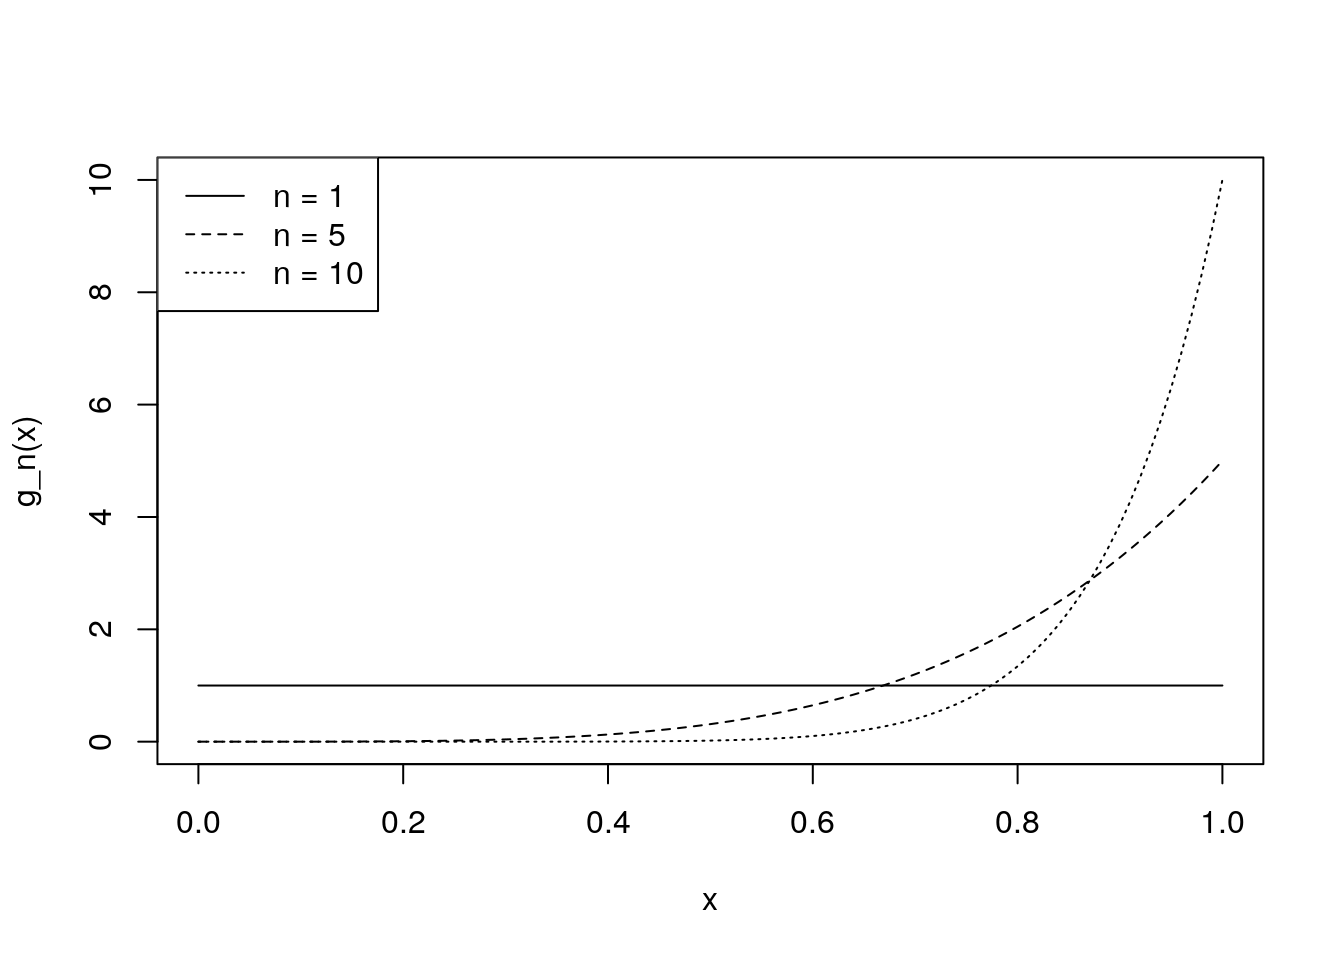
\includegraphics{MATH2011_files/figure-latex/unnamed-chunk-43-1.pdf}

As expected, we see that as \(n\) increases, it becomes more likely that
the maximum of the \(n\) \(U(0, 1)\) variables is close to \(1\).

\section{\texorpdfstring{The cdf of \(Y_{(1)}\), the smallest value in a
random sample of size
\(n\)}{The cdf of Y\_\{(1)\}, the smallest value in a random sample of size n}}\label{the-cdf-of-y_1-the-smallest-value-in-a-random-sample-of-size-n}

Since \(Y_{(1)} = \min\{Y_1, \ldots, Y_n\}\), the probability that
\(Y_{(1)} \leq y\) gives the cumulative distribution function of
\(Y_{(1)}\), the smallest value in the sample. Now

\begin{align*}
G_1(y) = P(Y_{(1)} \leq y) &= 1 - P(Y_{(1)} > y) \\
&= 1 - P(\text{all $Y_i > y$}) \\
&= 1 - P(Y_1 > y \text{ and } Y_2 > y \ldots \text{ and } Y_n > y) \\
&= 1 - P(Y_1 > y)P(Y_2 > y) \ldots P(Y_n > y) \\
&= 1 - [1 - F(y)]^n.
\end{align*}

by independence of the \(Y_i\).

\section{The pdf of the minimum in the continuous
case}\label{the-pdf-of-the-minimum-in-the-continuous-case}

If the \(Y_i\) are continuous, each with probability density function
\(f\), then the pdf of \(Y_{(1)}\) may be found by differentiating
\(G_1(y)\) with respect to \(y\) to give
\[g_1(y) = \frac{d}{dy} G_1(y) = n [1 - F(y)]^{n-1} f(y),\] where the
domain of the minimum is the same as that of each of the \(Y_i\).

\BeginKnitrBlock{example}[Minimum of an exponential random sample]
\protect\hypertarget{exm:expmin}{}{\label{exm:expmin} \iffalse (Minimum of
an exponential random sample) \fi{} }Suppose that each
\(Y_i \sim \text{Exp}(\theta)\), with pdf
\[f(y) = \theta e^{-\theta y}, \quad 0 < y < \infty\] and cdf
\[F(y) = \int_0^{y} f(u) du = 1 - e^{-\theta y}.\] Then
\(Y_{(1)} = \min\{Y_{(1)}, \ldots, Y_{(n)}\) has cdf
\[G_1(y) = 1 - [1 - F(y)]^n = 1 - e^{-n \theta y}\] and pdf
\[g_1(y) = \frac{d}{dy} G_1(y) = n \theta e^{-n \theta y}.\] So the the
distribution of the smallest value in an Exponential random sample of
size \(n\) with rate parameter \(\theta\) (i.e.~with mean value
\(1/\theta\)) is also an Exponential random variable but with rate
parameter \(n \theta\) (i.e.~with mean value \(1/(n\theta)\)).
\EndKnitrBlock{example}

This hints at some interesting structure in the probabilistic behaviour
of maxima and minima. The central limit theorem essentially says that
under certain conditions the sum of \(n\) independent, identically
distributed random variables is approximately normal as \(n\) grows
large. There are corresponding results for maxima and minima, though the
large-\(n\) distribution is not normal (it is the so-called generalised
extreme value distribution).

\chapter{The gamma distribution}\label{gamma}

\section{The gamma distribution}\label{the-gamma-distribution}

In this chapter we will introduce a family of distributions known as the
gamma distribution. We will see that this family contains several
sub-families of distributions that arise in practical problems,
including the exponential, chi-squared and Erlang distributions. The
gamma distribution is also related to normal, \(t\) and \(F\)
distributions.

In practice we are often interested in modelling data which is positive,
such as the time to the occurrence of an event of interest. We have seen
that an Exponential distribution is one possibility to model such data,
but it lacks flexibility --- it only has a single parameter and we have
seen that all exponential pdfs have the same shape (see Example
\ref{exm:homexp}). It is natural to try to generalise the exponential to
a more flexible family of distributions, and the gamma distribution is
one way of achieving this.

Before we introduce the gamma distribution, we first need to introduce a
function which is used in the pdf of the gamma distribution, to make
sure that the pdf integrates to one.

\BeginKnitrBlock{definition}[Gamma function]
\protect\hypertarget{def:unnamed-chunk-44}{}{\label{def:unnamed-chunk-44}
\iffalse (Gamma function) \fi{} }The \emph{Gamma function} is defined by
\[\Gamma(\alpha) = \int_0^\infty x^{\alpha - 1} e^{-x} dx.\]
\EndKnitrBlock{definition}

When \(\alpha = 1\), we have
\[\Gamma(1) = \int_0^\infty e^{-x} dx = 1.\]

Next, let's prove a useful property about the Gamma function.
\BeginKnitrBlock{proposition}
\protect\hypertarget{prp:gammarecursion}{}{\label{prp:gammarecursion} }For
any \(\alpha > 1\),
\(\Gamma(\alpha) = (\alpha - 1) \Gamma(\alpha - 1).\)
\EndKnitrBlock{proposition} \BeginKnitrBlock{proof}

\iffalse{} {Proof. } \fi{}We use integration by parts.

\begin{align*}
\Gamma(\alpha) &= \int_0^\infty x^{\alpha - 1} e^{-x} dx \\
&= \left[-x^{\alpha - 1} e^{-x}\right]_0^\infty
+ (\alpha - 1) \int_0^\infty x^{\alpha - 1} e^{-x}dx \\
&= 0 + (\alpha - 1)
\int_0^\infty x^{(\alpha - 1) - 1} e^{-x} dx \\
&= (\alpha - 1) \Gamma(\alpha - 1)
\end{align*}

since \(\alpha - 1 > 0\) as \(\alpha > 1\).
\EndKnitrBlock{proof}

As a consequence of Proposition \ref{prp:gammarecursion} and the fact
that \(\Gamma(1) = 1\), if \(\alpha\) is any positive integer then
\[\Gamma(\alpha) = (\alpha - 1)!,\] so the Gamma function can be thought
of as a continuous version of the factorial function.

It is also useful to know what happens to the Gamma function at half
integer points, \(\Gamma(1/2)\), \(\Gamma(3/2)\) and so on. It can be
shown that \[\Gamma(1/2) = \sqrt{\pi},\] and this may be used along with
the recurrence relationship (Proposition \ref{prp:gammarecursion}) to
compute any other \(\Gamma(n/2)\).

\BeginKnitrBlock{definition}
\protect\hypertarget{def:unnamed-chunk-46}{}{\label{def:unnamed-chunk-46}
}We say a random variable \(Y\) has \emph{gamma distribution} with
\emph{shape} parameter \(\alpha > 0\) and \emph{rate} parameter
\(\beta > 0\) if it has pdf

\begin{equation}
f(y) = \frac{\beta^\alpha}{\Gamma(\alpha)} y^{\alpha - 1} e^{-\beta y}, \quad y > 0.
\label{eq:gamma}
\end{equation}

We write this as \(Y \sim \text{gamma}(\alpha, \beta)\).
\EndKnitrBlock{definition}

Note that the exponential distribution with rate parameter \(\beta\) is
a special case of the gamma distribution, with \(\alpha = 1\).

\BeginKnitrBlock{example}[Time until the $k$th event in a Poisson process]
\protect\hypertarget{exm:unnamed-chunk-47}{}{\label{exm:unnamed-chunk-47}
\iffalse (Time until the \(k\)th event in a Poisson process) \fi{}
}Suppose we have a Poisson process with events arriving at rate
\(\beta\) per unit time, so that the number of events occurring in a
time interval of length \(t\) has \(\text{Poisson}(\beta t)\)
distribution. Let \(Y\) be the time until the \(k\)th event occurs. We
claim that \(Y \sim \text{gamma}(k, \beta)\).

Let \(N_y\) be the number of events in the time interval \((0, y]\).
Then \(N_y \sim \text{Poisson}(\beta y)\). We have
\[P(Y > y) = P(N_y \leq k - 1) = \sum_{n=0}^{k-1} \frac{(\beta y)^n e^{-\beta y}}{n!},\]
so

\begin{align*}
F(y) = P(Y \leq y) &= 1- P(Y > y) \\
&= 1 - \sum_{n=0}^{k-1} \frac{(\beta y)^n e^{-\beta y}}{n!} \\
&= 1 - e^{-\beta y} -  \sum_{n=1}^{k-1} \frac{(\beta y)^n e^{-\beta y}}{n!}.
\end{align*}

So

\begin{align*}
f(y) &= \frac{dF}{dy} = \beta e^{-\beta y} - 
\sum_{n=1}^{k-1} \left\{ \frac{\beta^n y^{n-1} e^{-\beta y}}{(n-1)!} 
- \beta \frac{(\beta y)^n}{n!} e^{-\beta y} \right\} \\
&= \beta e^{-\beta y} - \beta e^{-\beta y} 
+ \beta^2 y e^{-\beta y} - \beta^2 y e^{-\beta y}
+ \frac{\beta^3 y^2}{2!} e^{-\beta y} - \ldots + \frac{\beta (\beta y)^{k-1}}{(k-1)!} e^{-\beta y} \\
&= \frac{\beta^k}{\Gamma(k)} y^{k-1} e^{-\beta y},
\end{align*}

which is the pdf of a \(\text{gamma}(k, \beta)\) random variable.

If \(\alpha\) is an integer, as in this example, the
\(\text{gamma}(\alpha, \beta)\) distribution is also known as the
\emph{Erlang} distribution. The exponential distribution (with
\(\alpha= 1\)) is a special case of the Erlang distribution.
\EndKnitrBlock{example}

\section{Properties of the gamma
distribution}\label{properties-of-the-gamma-distribution}

\BeginKnitrBlock{proposition}
\protect\hypertarget{prp:mgfgamma}{}{\label{prp:mgfgamma} }The moment
generating function of the \(\text{gamma}(\alpha, \beta)\) distribution
is
\[M_Y(t) = \left(1 - \frac{t}{\beta} \right)^{-\alpha}, \quad \text{for $t < \beta$}\]
\EndKnitrBlock{proposition} \BeginKnitrBlock{proof}

\iffalse{} {Proof. } \fi{}We have

\begin{align*}
M_Y(t) = E(e^{tY}) &= \int_0^\infty e^{ty} 
\frac{\beta^\alpha}{\Gamma(\alpha)} y^{\alpha - 1} e^{-\beta y} dy \\
&= \int_0^\infty \frac{\beta^\alpha}{\Gamma(\alpha)} y^{\alpha - 1} e^{-y(\beta - t)} dy \\
&= \frac{\beta^\alpha}{(\beta - t)^\alpha} \int_0^\infty \frac{(\beta - t)^\alpha}{\Gamma(\alpha)} y^{\alpha - 1} e^{-y(\beta - t)} dy \\
&= \left(1 - \frac{t}{\beta}\right)^{-\alpha} \times 1,
\end{align*}

as the final integrand is the pdf of a
\(\text{gamma}(\alpha, \beta - t)\) distribution, which integrates to
\(1\) provided that the new rate parameter \(\beta - t > 0\), i.e.~if
\(t < \beta\).
\EndKnitrBlock{proof}

The following proposition tells us that the gamma distribution is always
positively skewed, but the skewness decreases as \(\alpha\) increases.
The gamma distribution always has larger kurtosis than the normal
distribution, but the kurtosis decreases towards the kurtosis of a
normal distribution (\(\gamma_2 = 3\)) as \(\alpha\) increases.

\BeginKnitrBlock{proposition}
\protect\hypertarget{prp:gammamoments}{}{\label{prp:gammamoments} }Suppose
\(Y \sim \text{gamma}(\alpha, \beta)\). Then
\(E(Y) = \alpha \beta^{-1}\) and \(\text{Var}(Y) = \alpha \beta^{-2}\).
The skewness is \(\gamma_1 = 2 \alpha^{-1/2}\) and the kurtosis is
\(\gamma_2 = 3 + 6 \alpha^{-1}\).
\EndKnitrBlock{proposition} \BeginKnitrBlock{proof}

\iffalse{} {Proof. } \fi{}From Proposition \ref{prp:mgfgamma}, the mgf
is \(M_Y(t) = (1 - t/\beta)^{-\alpha}\), the the cgf is
\(K_Y(t) = \log M_Y(t) = -\alpha \log(1 - t/\beta)\). Differentiating,
we have
\[K_Y^{(1)}(t) = \frac{\alpha}{\beta\left(1 - \frac{t}{\beta}\right)} = \frac{\alpha}{\beta - t},\]
so \(E(Y) = K_Y^{(1)}(0) = \alpha \beta^{-1}\).

Differentiating the cgf again,
\[K_Y^{(2)}(t) = \frac{d}{dt} \left[\alpha (\beta - t)^{-1}\right]
= \alpha(\beta - t)^{-2},\] so
\(\mu_2 = \text{Var}(Y) = K_Y^{(2)}(0) = \alpha \beta^{-2}\).

Differentiating the cgf again,
\[K_Y^{(3)}(t) = \frac{d}{dt} \left[\alpha (\beta - t)^{-2}\right] 
= 2 \alpha (\beta - t)^{-3},\] so the third moment about the mean is
\(\mu_3 = K_Y^{(3)}(0) = 2 \alpha \beta^{-3}\). So the skewness is
\[\gamma_1 = \frac{\mu_3}{\mu_2^{3/2}}
= \frac{2 \alpha \beta^{-3}}{[\alpha \beta^{-2}]^{3/2}} = 2 \alpha^{-1/2}.\]

Differentiating the cgf again,
\[K_Y^{(4)}(t) = \frac{d}{dt} \left[2 \alpha (\beta - t)^{-3}\right] 
= 6 \alpha (\beta - t)^{-4},\] so the fourth cumulant is
\(\kappa_4 = 6 \alpha \beta^{-4}\). The fourth moment about the mean is
\[\mu_4 = \kappa_4 + 3 \mu_2^2 = 6 \alpha \beta^{-4} + 3 \alpha^2 \beta^{-4},\]
so the kurtosis is
\[\gamma_2 = \frac{\mu_4}{\mu_2^2} = 3 + \frac{6 \alpha \beta^{-4}}{\alpha^2 \beta^{-4}} = 3 + 6 \alpha^{-1},\]
as claimed.
\EndKnitrBlock{proof}

The gamma distribution is closed under scaling, and under summation of
independent gamma distributions with a common rate parameter.

\BeginKnitrBlock{proposition}
\protect\hypertarget{prp:gammascale}{}{\label{prp:gammascale} }Suppose
\(Y \sim \text{gamma}(\alpha, \beta)\), and let \(Z = bY\), for some
constant \(b > 0\). Then \(Z \sim \text{gamma}(\alpha, \beta / b)\).
\EndKnitrBlock{proposition} \BeginKnitrBlock{proof}

\iffalse{} {Proof. } \fi{}By Theorem \ref{thm:gflinear}, we have
\[M_Z(t) = M_Y(bt) = \left( 1 - \frac{bt}{\beta} \right)^{-\alpha}
= \left(1 - \frac{t}{\beta/b}\right)^{-\alpha},\] which is the mgf of a
\(\text{gamma}(\alpha, \beta / b)\) distribution. Since the mgf
characterises the distribution, we have
\(Z \sim \text{gamma}(\alpha, \beta / b)\).
\EndKnitrBlock{proof}

\BeginKnitrBlock{proposition}
\protect\hypertarget{prp:gammasum}{}{\label{prp:gammasum} }If
\(Y_1, \ldots, Y_n\) are independent, with
\(Y_i \sim \text{gamma}(\alpha_i, \beta)\) then
\(Z = \sum_{i=1}^n Y_i \sim \text{gamma}(\sum_{i=1}^n \alpha_i, \beta)\).
\EndKnitrBlock{proposition} \BeginKnitrBlock{proof}

\iffalse{} {Proof. } \fi{}By Theorem \ref{thm:mgfsum}, we have

\begin{align*}
M_Z(t) &= \prod_{i=1}^n M_{Y_i}(t) \\
&= \prod_{i=1}^n \left( 1 - \frac{t}{\beta} \right)^{-\alpha_i}
&= \left( 1 - \frac{t}{\beta} \right)^{-\sum_{i=1}^n \alpha_i},
\end{align*}

which is the mgf of a \(\text{gamma}(\sum_{i=1}^n \alpha_i, \beta)\)
distribution. Since the mgf characterises the distribution, we have
\(Z \sim \text{gamma}(\sum_{i=1}^n \alpha_i, \beta)\).
\EndKnitrBlock{proof}

\section{The chi-squared distribution}\label{chisquared}

The chi-squared distribution is a useful special case of the gamma
distribution.

\BeginKnitrBlock{definition}
\protect\hypertarget{def:chisquared}{}{\label{def:chisquared} }We say a
random variable \(Y\) has \emph{chi-squared} distribution with \(n\)
degrees of freedom if \(Y \sim \text{gamma}(n/2, 1/2)\). We write
\(Y \sim \chi^2_n\).
\EndKnitrBlock{definition} We can write down the properties of the
chi-squared distribution by using results we have already proved about
the gamma distribution.

If \(Y \sim \chi^2_n\), we have
\[E(Y) = \frac{n/2}{1/2} = n; \qquad \text{Var}(Y) = \frac{n/2}{(1/2)^2}  = 2n.\]

By Proposition \ref{prp:gammasum}, if \(Y_1, \ldots, Y_n\) are
independent random variables, with \(Y_i \sim \chi^2_{n_i}\) then

\begin{equation}
\sum_{i=1}^n Y_i \sim \chi^2_{\sum_{i=1}^n n_i}.
\label{eq:chisquaredsum}
\end{equation}

The \emph{sum of independent chi-squared random variables} has
chi-squared distribution with degrees of freedom given by the \emph{sum
of the individual degrees of freedom}.

The chi-squared distribution is also related to the normal distribution.
\BeginKnitrBlock{proposition}
\protect\hypertarget{prp:chisquarednormal}{}{\label{prp:chisquarednormal}
}Let \(Z \sim N(0, 1)\), and let \(Y = Z^2\). Then \(Y \sim \chi^2_1\).
\EndKnitrBlock{proposition}

\BeginKnitrBlock{proof}
\iffalse{} {Proof. } \fi{}Write \(\Phi(.)\) for the cumulative
distribution function of \(Z\), and \(\phi(.)\) for the pdf of \(Z\), so
that
\[\phi(z) = \frac{1}{\sqrt{2 \pi}} \exp\left(-\frac{z^2}{2}\right).\]
Let \(Y\) have cdf \(F(.)\) and pdf \(f(.)\). Then, for \(y > 0\),

\begin{align*}
F(y) &= P(Y \leq y) = P(Z^2 \leq y) \\
&= P\left(-\sqrt{y} \leq Z \leq \sqrt{y} \right) \\
&= \Phi\left(\sqrt{y}\right) - \Phi\left(-\sqrt{y}\right).
\end{align*}

So

\begin{align*}
f(y) &= \frac{d}{dy} F(y) 
= \frac{1}{2 \sqrt{y}} \phi \left(\sqrt{y}\right) 
+ \frac{1}{2 \sqrt{y}} \phi \left(-\sqrt{y}\right) \\
&= \frac{1}{2 \sqrt{y}} \left\{\frac{1}{\sqrt{2 \pi}} \exp\left(-\frac{y}{2}\right) + \frac{1}{\sqrt{2 \pi}} \exp\left(-\frac{y}{2}\right) \right\} \\
&= \frac{1}{\sqrt{2}\sqrt{y}\sqrt{\pi}} \exp\left(-\frac{y}{2}\right) \\
&= \frac{y^{\frac{1}{2} - 1}}{\Gamma(1/2)} 
\left(\frac{1}{2}\right)^{1/2} \exp\left(-\frac{y}{2}\right),
\end{align*}

since \(\Gamma(1/2) = \sqrt{\pi}\). This is the pdf of a
\(\text{gamma}(1/2, 1/2) \equiv \chi^2_1\) distribution, as claimed.
\EndKnitrBlock{proof} Putting together Proposition
\ref{prp:chisquarednormal} and Equation \eqref{eq:chisquaredsum} gives us
a way to construct a random variable with any chi-squared distribution,
given a supply of independent and identically distributed standard
normal random variables: \BeginKnitrBlock{proposition}

\protect\hypertarget{prp:chisquaredsumnormal}{}{\label{prp:chisquaredsumnormal}
}Let \(Z_1, Z_2, \ldots Z_n\) be independent and identically
distributed, with \(Z_i \sim N(0, 1)\), and let
\(Y = \sum_{i=1}^n Z_i^2\). Then \(Y \sim \chi^2_n\).
\EndKnitrBlock{proposition} \BeginKnitrBlock{proof}

\iffalse{} {Proof. } \fi{}By Proposition \ref{prp:chisquarednormal},
each \(Z_i^2 \sim \chi^2_1\), and \(Z_1^2, \ldots, Z_n^2\) are
independent. So by Equation \eqref{eq:chisquaredsum} with \(n_i = 1\),
\(Y \sim \chi^2_{\sum_{i=1}^n 1} \equiv \chi^2_n\), as claimed.
\EndKnitrBlock{proof}

\section{Distribution of the sample
variance}\label{distribution-of-the-sample-variance}

Suppose \(Y_1, Y_2, \ldots, Y_n\) are independent identically
distributed \(N(\mu, \sigma^2)\) random variables. We can use
observations of \(y_1, y_2, \ldots, y_n\) of \(Y_1, \ldots, Y_n\) to
estimate \(\mu\) and \(\sigma^2\). We can use the sample mean
\[\bar y = \frac{1}{n} \sum_{i=1}^n y_i\] to estimate \(\mu\), and the
sample variance \[s^2 = \frac{\sum_{i=1}^n (y_i - \bar y)^2}{n-1}\] to
estimate \(\sigma^2\).

For any specific sample of observations, \(\bar y\) and \(s^2\) will
take specific numerical values, but when they are defined in terms of
the random variables \(Y_1 , Y_2 , \ldots, Y_n\), they too are random
variables and will have distributions.

We have already seen (in Proposition \ref{prp:ybarnormal}) that
\(\bar Y \sim N(\mu, \sigma^2/n)\). We would like to also know the
distribution of the random version of the sample variance

\begin{equation}
S^2 = \frac{\sum_{i=1}^n (Y_i - \bar Y)^2}{n-1}.
\label{eq:S2}
\end{equation}

\BeginKnitrBlock{theorem}
\protect\hypertarget{thm:S2dist}{}{\label{thm:S2dist}
}\(Y_1, Y_2, \ldots, Y_n\) are independent identically distributed
\(N(\mu, \sigma^2)\) random variables, and let \(S^2\) be as defined in
Equation \eqref{eq:S2}. Then
\[\frac{(n-1)S^2}{\sigma^2} \sim \chi^2_{n-1},\] and \(S^2\) and
\(\bar Y\) are independent.
\EndKnitrBlock{theorem}

In order to prove this important result, we will need to use Cochran's
theorem, which we state here without proof.

\BeginKnitrBlock{theorem}[Cochran's Theorem]
\protect\hypertarget{thm:cochran}{}{\label{thm:cochran} \iffalse (Cochran's
Theorem) \fi{} }Suppose that \(U \sim \text{gamma}(\alpha_1, \beta)\)
and \(W \sim \text{gamma}(\alpha_1 + \alpha_2, \beta)\). If
\(V = W - U\), then any one of the following implies the other two:

\begin{enumerate}
\def\labelenumi{\roman{enumi})}
\tightlist
\item
  \(V \sim \text{gamma}(\alpha_2, \beta)\).
\item
  \(V\) is independent of \(U\)
\item
  \(V\) is non-negative.
\end{enumerate}
\EndKnitrBlock{theorem}

We use Cochran's theorem to prove Theorem \ref{thm:S2dist}:

\BeginKnitrBlock{proof}[Theorem \@ref(thm:S2dist)]
\iffalse{} {Proof (Theorem \ref{thm:S2dist}). } \fi{}The key to the
proof is to write \(\sum_{i=1}^n (Y_i - \bar Y)^2\) in terms of
\(\sum_{i=1}^n (Y_i - \mu)^2\). We have

\begin{align*}
\sum_{i=1}^n (Y_i - \mu)^2 &= \sum_{i=1}^n (Y_i - \bar Y + \bar Y - \mu)^2 \\
&= \sum_{i=1}^n \left\{(Y_i - \bar Y)^2 
+ 2(Y_i - \bar Y)(\bar Y - \mu) + (\bar Y - \mu)^2 \right\} \\
&= \sum_{i=1}^n (Y_i - \bar Y)^2 + 
2(\bar Y - \mu) \sum_{i=1}^n (Y_i - \bar Y) + n(\bar Y - \mu)^2 \\
&= \sum_{i=1}^n (Y_i - \bar Y)^2 + n(\bar Y - \mu)^2,
\end{align*}

as \(\sum_{i=1}^n (Y_i - \bar Y) = 0\). So
\[\sum_{i=1}^n (Y_i - \mu)^2  = \sum_{i=1}^n (Y_i - \bar Y)^2 - n(\bar Y - \mu)^2.\]
Multiplying through by \(\frac{1}{\sigma^2}\) gives
\[\frac{1}{\sigma^2}\sum_{i=1}^n (Y_i - \mu)^2 = \frac{1}{\sigma^2}\sum_{i=1}^n (Y_i - \bar Y)^2 - \frac{n}{\sigma^2}(\bar Y - \mu)^2,\]
so \[\frac{(n-1)S^2}{\sigma^2} 
= \sum_{i=1}^n \left(\frac{Y_i - \mu}{\sigma}\right)^2 
- \left(\frac{\sqrt{n}(\bar Y - \mu)}{\sigma} \right)^2.\] But
\((Y_i - \mu)/\sigma \sim N(0, 1)\), so
\[\sum_{i=1}^n \left(\frac{Y_i - \mu}{\sigma}\right)^2 
\sim \chi^2_n\] by Proposition \ref{prp:chisquaredsumnormal}. We have
\(\sqrt{n}(\bar Y - \mu)/\sigma \sim N(0, 1)\) by Proposition
\ref{prp:ybarnormal}, so
\[\left(\frac{\sqrt{n}(\bar Y - \mu)}{\sigma} \right)^2 
\sim \chi^2_1\] by Proposition \ref{prp:chisquarednormal}.

Now we use Cochran's Theorem (\ref{thm:cochran}), with

\begin{align*}
V &= \frac{(n-1) S^2}{\sigma^2} \\
W &= \sum_{i=1}^n \left(\frac{Y_i - \mu}{\sigma}\right)^2 
\sim \chi^2_n \equiv \text{gamma}(n/2, 1/2) \\
U &= \left(\frac{\sqrt{n}(\bar Y - \mu)}{\sigma} \right)^2 
\sim \chi^2_1 \equiv \text{gamma}(1/2, 1/2),
\end{align*}

so \(\alpha_1 = 1/2\) and \(\alpha_1 + \alpha_2 = n/2\), so
\(\alpha_2 = (n-1)/2\). We have \(\sum_{i=1}^n (Y_i - \bar Y) \geq 0\),
so \(V \geq 0\), so condition (iii) in Cochran's Theorem is met.

So by (ii) of Cochran's Theorem, \(V = \frac{(n-1) S^2}{\sigma^2}\) is
independent of
\(U = \left(\frac{\sqrt{n}(\bar Y - \mu)}{\sigma} \right)^2\), and hence
\(S^2\) is independent of \(\bar Y\), as claimed.

By (i) of Cochran's Theorem, \[V = \frac{(n-1) S^2}{\sigma^2} 
\sim \text{gamma}(\alpha_2, 1/2)
\equiv \text{gamma}((n-1)/2, 1/2) \equiv \chi^2_{n-1},\] as claimed.
\EndKnitrBlock{proof}

A consequence of Theorem \ref{thm:S2dist} is that

\begin{align*}
E(S^2) &= E\left(\frac{\sigma^2}{n-1} \frac{(n-1) S^2}{\sigma^2} \right) \\
  &= \frac{\sigma^2}{n-1} E\left(\frac{(n-1) S^2}{\sigma^2} \right) \\
  &=  \frac{\sigma^2}{n-1} \cdot (n - 1) = \sigma^2,
  \end{align*}

where we have used that the expected value of a chi-squared random
variable is its degrees of freedom. So \(S^2\) is an \emph{unbiased}
estimator of \(\sigma^2\): a concept which we will revisit in Chapter
\ref{estimation}.

\chapter{Univariate transformations}\label{unitransform}

\section{Transformed random
variables}\label{transformed-random-variables}

In this chapter, starting with a random variable \(Y\), we define a new
random variable \(U = U(Y)\). We want to be able to determine the
distribution of the transformed random variable \(U\).

We have already studied one method for finding the distribution of a
transformed random variable, when that transformation is linear
(\(U = a + bY\) for suitable constants \(a\) and \(b\)). In that case,
if we have the moment generating function of \(Y\), we can use Theorem
\ref{thm:gflinear} to find the moment generating function of \(U\).

However, we are often interested in non-linear transformations. For
example, we have seen (in Proposition \ref{prp:chisquarednormal}) an
example where we squared a \(N(0, 1)\) random variables to obtain a new
random variable with \(\chi^2_1\) distribution, i.e.~we had a
transformation of the form \(U = Y^2\).

We begin with two simple examples.

\BeginKnitrBlock{example}
\protect\hypertarget{exm:trans1}{}{\label{exm:trans1} }Suppose \(Y\) has pdf
\[f(y) = 2y, \quad \text{for $0 < y < 1$}.\] Let \(U = Y^2\). What is
the distribution of \(U\)?

Let \(G(.)\) and \(g(.)\) be the cdf and pdf of \(U\). We have
\[G(u) = P(U \leq u) = P(Y^2 \leq u) 
= P(Y \leq \sqrt{u}) = F(\sqrt{u}).\] So

\begin{align*}
g(u) &= \frac{dG(u)}{du} = \frac{dF(\sqrt{u})}{du} 
= f(\sqrt{u}) \frac{1}{2 \sqrt{u}} \\
&= 2 \sqrt{u} \frac{1}{2 \sqrt{u}} 
= 1 \quad \text{for $0 < u < 1$,}
\end{align*}

which is the pdf of a \(U(0, 1)\) distribution. So \(U \sim U(0, 1)\).
\EndKnitrBlock{example}

\BeginKnitrBlock{example}
\protect\hypertarget{exm:trans2}{}{\label{exm:trans2} }Suppose
\(Y \sim U(0, 1)\). Let \(U = -\log{Y}\). What is the distribution of
\(U\)?

Let \(G(.)\) and \(g(.)\) be the cdf and pdf of \(U\). We have

\begin{align*}
G(u) &= P(U \leq u) = P(\log Y \leq u) \\
&= P(\log Y \geq -u) = P(Y \geq e^{-u}) \\
&= 1 - P(Y < e^{-u}) = 1 - F(e^{-u}) \\
&= 1 - e^{-u}, \quad \text{for $0 < u < \infty$.}
\end{align*}

So \[g(u) = \frac{dG(u)}{du} = e^{-u}, \quad \text{for $u > 0$},\] which
we recognise as the pdf of an exponential distribution with rate
parameter \(1\), so \(U \sim \text{exponential}(1)\).
\EndKnitrBlock{example}

\section{One-to-one transformations of continuous random
variables}\label{one-to-one-transformations-of-continuous-random-variables}

\BeginKnitrBlock{theorem}
\protect\hypertarget{thm:unitrans}{}{\label{thm:unitrans} }If \(U\) is a
one-to-one transformation of a continuous random variable \(Y\), the pdf
of \(U\) is \[g(u) = f(w(u)) \left|\frac{dy}{du} \right|\] where Y =
w(U) is the inverse transformation.
\EndKnitrBlock{theorem} \BeginKnitrBlock{remark}

\iffalse{} {Remark. } \fi{}In Example \ref{exm:trans1}, \(U = Y^2\), so
the inverse transformation is \(Y = U^{1/2} = w(U)\). In Example
\ref{exm:trans2}, \(U = -\log Y\), so the inverse transformation is
\(Y = \exp(-U) = w(U)\).
\EndKnitrBlock{remark} \BeginKnitrBlock{remark}

\iffalse{} {Remark. } \fi{}If the domain of \(Y\) is \((a, b)\), then
the domain of \(U\) is all values of \(u\) such that \(a < w(u) < b\)
(where \(a\) and \(b\) might be infinite).
\EndKnitrBlock{remark}
\BeginKnitrBlock{proof}[Theorem \@ref(thm:unitrans)]
\iffalse{} {Proof (Theorem \ref{thm:unitrans}). } \fi{}Let \(F(.)\) and
\(f(.)\) be the cdf and pdf of \(Y\), and let \(G(.)\) and \(g(.)\) be
the cdf and pdf of \(U\). Suppose \(U = h(Y)\) is a one-to-one function
with inverse \(Y = w(U)\). Since \(h(.)\) is one-to-one, we may conclude
that is is either an increasing or a decreasing function, and we split
the proof into two cases.

\textbf{Case 1}: \(h(.)\) is an increasing function. Then
\[G(u) = P(U \leq u) = P(h(Y) \leq u) 
= P(Y \leq w(u)),\] since \(h(.)\) is increasing. So \(G(u) = F(w(u))\),
and \[g(u) = f\left(w(u)\right) \frac{dw(u)}{du}
= f\left(w(u)\right) \frac{dy}{du}
= f\left(w(u)\right) \left|\frac{dy}{du}\right|,\] since
\(\frac{dy}{du} > 0\).

\textbf{Case 2}: \(h(.)\) is a decreasing function. Then
\[G(u) = P(U \leq u) = P(h(Y) \leq u) 
= P(Y \geq w(u)),\] since \(h(.)\) is decreasing. So
\(G(u) = 1 - F(w(u))\), and
\[g(u) = - f\left(w(u)\right) \frac{dw(u)}{du}
= f\left(w(u)\right) \left(- \frac{dy}{du}\right)
= f\left(w(u)\right) \left|\frac{dy}{du}\right|,\] since
\(\frac{dy}{du} < 0\).
\EndKnitrBlock{proof}

\BeginKnitrBlock{example}[Kinetic energy of gas molecules]
\protect\hypertarget{exm:unnamed-chunk-58}{}{\label{exm:unnamed-chunk-58}
\iffalse (Kinetic energy of gas molecules) \fi{} }Gas molecules move
about with varying velocity which has, according to the
Maxwell-Boltzmann law, a pdf given by
\[f(v) = c v^2 e^{-\beta v^2}, \quad v > 0,\] where \(c\) is a constant
to ensure the pdf integrates to \(1\). The kinetic energy is given by
\(U = \frac{1}{2} m V^2\), where \(m\) is the mass of the molecule. What
is the pdf of \(U\), the kinetic energy of the molecule?

The domain of \(U\) is \(0 < u < \infty\). For \(v > 0\),
\(h(v) = \frac{1}{2} m v^2\) is a one-to-one function, as it is
increasing with \(v\). So we may apply Theorem \ref{thm:unitrans} to
find the pdf \(g(.)\) of \(U\).

We have \(u = \frac{1}{2} m v^2\), so the inverse transformation is
\(v = \sqrt{\frac{2u}{m}}\), and
\[\frac{dv}{du} = \frac{\sqrt{2}}{2 \sqrt{um}} = \frac{1}{\sqrt{2 u m}} > 0
\quad \text{for $u > 0$}.\] So \(U\) has pdf

\begin{align*}
g(u) &= f \left(\sqrt{\frac{2u}{m}} \right) \frac{1}{\sqrt{2um}} \\
&= c \cdot \frac{2u}{m} e^{-\beta\frac{2u}{m}} \frac{1}{\sqrt{2um}} \\
&= c \sqrt{2u} m^{-\frac{3}{2}}e^{-\beta\frac{2u}{m}}
\quad \text{for $u > 0$.}
\end{align*}

We see that \[g(u) \propto u^{\frac{1}{2}} e^{-\beta\frac{2u}{m}} 
= u^{\frac{3}{2} - 1} e^{-\theta u}\] with \(\theta = 2\beta / m\). So,
by comparison with Equation \eqref{eq:gamma},
\(U \sim \text{gamma}(3/2, 2 \beta/m)\).
\EndKnitrBlock{example}

\section{Generating samples from any
distribution}\label{generating-samples-from-any-distribution}

\BeginKnitrBlock{proposition}
\protect\hypertarget{prp:cdfconttrans}{}{\label{prp:cdfconttrans} }Suppose
that \(Y\) is a continuous random variable with cumulative distribution
function \(F(.)\). Let \(U = F(Y)\). Then \(U \sim U(0, 1)\).
\EndKnitrBlock{proposition} \BeginKnitrBlock{proof}

\iffalse{} {Proof. } \fi{}\(U\) has cdf

\begin{align*}
G(u) &= P(U \leq u) = P(F(Y) \leq u) \\
&= P(Y \leq F^{-1}(u)) \quad \text{since $F(.)$ is increasing} \\
&= F\left(F^{-1}(u)\right) = u \quad \text{for $0 < u < 1$},
\end{align*}

which is the cdf of a \(U(0, 1)\) distribution. So \(U \sim U(0, 1)\),
as required.
\EndKnitrBlock{proof}

An immediate corollary of Proposition \ref{prp:cdfconttrans} allows us
to use a sample from a \(U(0, 1)\) distribution to generate a sample
from any other continuous distribution:

\BeginKnitrBlock{corollary}
\protect\hypertarget{cor:inversetranscont}{}{\label{cor:inversetranscont}
}Let \(F(.)\) be the cumulative distribution function of a continuous
distribution, with inverse \(F^{-1}(.)\). Suppose that
\(U \sim U(0, 1)\). Then \(Y = F^{-1}(U)\) has cumulative distribution
function \(F(.)\).
\EndKnitrBlock{corollary}

\BeginKnitrBlock{example}
\protect\hypertarget{exm:unnamed-chunk-60}{}{\label{exm:unnamed-chunk-60}
}Suppose that you are given \(U \sim N(0, 1)\), and would like to
generate \(Y \sim \text{exponential}(2)\). The \(\text{exponential}(2)\)
distribution has cdf \[F(y) = 1 - e^{-2y}, \quad \text{for $y > 0$,}\]
and inverting (solving \(u = F(y)\) for \(y\)) gives
\[F^{-1}(u) = -\frac{1}{2} \log(1 - u).\] So
\[Y = -\frac{1}{2} \log(1 - u) \sim \text{exponential}(2).\]
\EndKnitrBlock{example}

In fact, we can use the same method to find samples from a discrete
distribution. To do this, we first need to define what we mean by
\(F^{-1}(.)\), as the cdf \(F(.)\) is constant between points in the
domain, and so is not an invertible function.

For instance, if \(Y \sim \text{binomial}(2, 0.5)\), then we can plot
the cdf of \(Y\):

\begin{Shaded}
\begin{Highlighting}[]
\KeywordTok{curve}\NormalTok{(}\KeywordTok{pbinom}\NormalTok{(x, }\DecValTok{2}\NormalTok{, }\FloatTok{0.5}\NormalTok{), }\DataTypeTok{from =} \DecValTok{-1}\NormalTok{, }\DataTypeTok{to =} \DecValTok{3}\NormalTok{,}
      \DataTypeTok{xlab =} \StringTok{"y"}\NormalTok{, }\DataTypeTok{ylab =} \StringTok{"cdf F(y)"}\NormalTok{, }\DataTypeTok{n =} \DecValTok{1001}\NormalTok{)}
\end{Highlighting}
\end{Shaded}

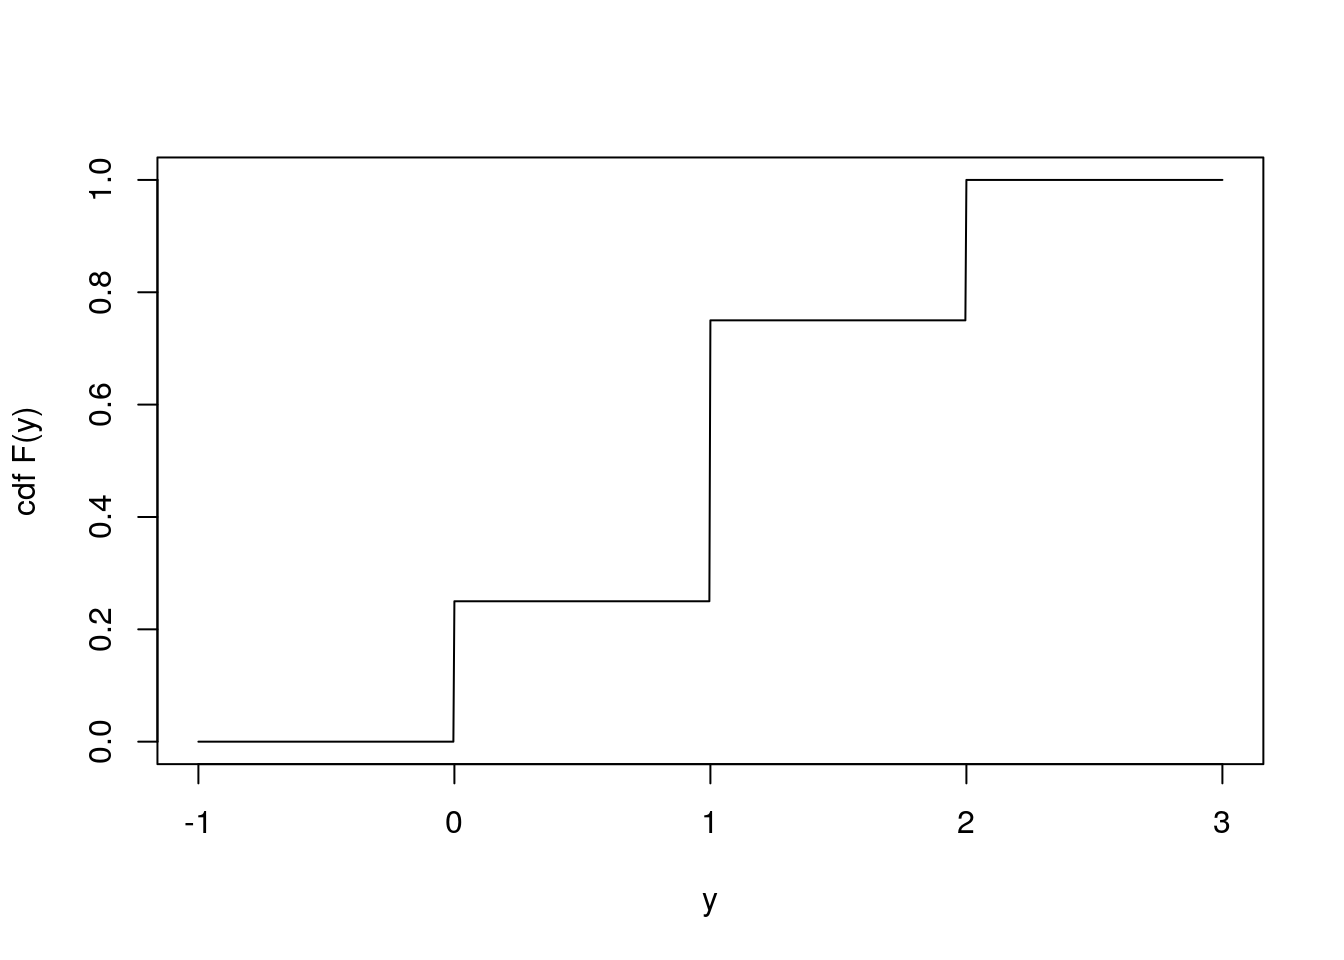
\includegraphics{MATH2011_files/figure-latex/unnamed-chunk-61-1.pdf}

In this example, if we ask for \(F^{-1}(0.25)\), then it is not
immediately clear what this means, as \(F(y) = 0.25\) for all
\(0 \leq y < 1\).

We define \(F^{-1}(.)\) by the \emph{quantile} function

\begin{equation}
F^{-1}(u) = \inf\{y \in \mathbb{R}: F(y) \geq u\},
\label{eq:quantile}
\end{equation}

for \(u \in (0, 1)\). In our example, we now have \(F^{-1}(0.25) = 0\).
If \(F(.)\) is an invertible function, then this definition agrees with
the usual inverse we saw before.

Equipped with this definition of \(F^{-1}(.)\), we may now rewrite
Corollary \ref{cor:inversetranscont} to apply to any distribution:
\BeginKnitrBlock{corollary}
\protect\hypertarget{cor:unnamed-chunk-62}{}{\label{cor:unnamed-chunk-62}
}Let \(F(.)\) be a cumulative distribution function, and let
\(F^{-1}(.)\) be the corresponding quantile function, defined by
\eqref{eq:quantile}. Suppose that \(U \sim U(0, 1)\). Then
\(Y = F^{-1}(U)\) has cumulative distribution function \(F(.)\).
\EndKnitrBlock{corollary}

\BeginKnitrBlock{example}[Generating a binomial random variable]
\protect\hypertarget{exm:unnamed-chunk-63}{}{\label{exm:unnamed-chunk-63}
\iffalse (Generating a binomial random variable) \fi{} }Suppose that you
are given \(U \sim N(0, 1)\), and would like to generate
\(Y \sim \text{binomial}(2, 0.5)\). The \(\text{binomial}(2)\)
distribution has cdf \[F(y) = \begin{cases} 
0 & \text{for $y < 0$} \\
0.25 & \text{for $0 \leq y < 1$} \\
0.75 & \text{for $1 \leq y < 2$} \\
1 & \text{for $y > 1$.}
\end{cases}\] The corresponding quantile function is
\[F^{-1}(u) = \begin{cases} 
-\infty & \text{for $u \leq 0$} \\
0 & \text{for $0 < u \leq 0.25$} \\
1 & \text{for $0.25 < u \leq 0.75$} \\
2 & \text{for $0.75 < u \leq 1$} \\
\infty & \text{for $u > 1$.}
\end{cases}\] So \(Y = F^{-1}(U) \sim \text{binomial}(2, 0.5)\).
\EndKnitrBlock{example}

\chapter{Bivariate distributions}\label{bivariate-distributions}

\section{Joint distributions}\label{joint-distributions}

There are many situations where random variables vary simultaneously,
for example:

\begin{itemize}
\tightlist
\item
  height and weight of individuals in a population
\item
  systolic and diastolic blood pressure of individuals in a population
\item
  value of Sterling and the Euro in US Dollars today at 12.00 GMT
\end{itemize}

In these cases and in many other situations, the variables are not
independent so we need to consider their \emph{joint behaviour}.

Under some circumstances it might be possible to assume or to deduce
that the variables do not depend on each other, i.e.~that they are
independent. We need to define the joint probabilistic behaviour of two
random variables. We could define these terms for either discrete or
continuous random variables. However, we give the definitions in terms
of continuous random variables with obvious extensions to the discrete
or other cases.

We could generalise these results when we have several random variables
(giving so-called multivariate models) but here we shall concentrate on
the simplest case of two random variables (the bivariate case).

Suppose \(Y_1\) and \(Y_2\) vary together with joint probability density
function \(f(y_1 , y_2)\). The function \(f\) has the following
properties:

\begin{enumerate}
\def\labelenumi{\arabic{enumi}.}
\tightlist
\item
  \(f(y_1, y_2) \geq 0\) for all \(y_1, y_2\).
\item
  \(\int_{a_1}^{b_1} \int_{a_2}^{b_2} f(y_1, y_2) dy_1 dy_2 = P(a_1 < Y_1 \leq b_1 \text{ and } a_2 < Y_2 \leq b_2)\).
\end{enumerate}

An immediate corollary is that
\(\int_{-\infty}^{\infty} \int_{-\infty}^{\infty} f(y_1, y_2) dy_1 dy_2 = 1\).

We will give some examples shortly, but first we set up some more
functions of interest.

The \emph{marginal} probability density function of \(Y_1\) is given by
integrating out \(Y_2\) , i.e.
\[f_1(y_1) = \int_{-\infty}^\infty f(y_1, y_2) dy_2.\] This essentially
gives the probabilistic behaviour of \(Y_1\) ignoring \(Y_2\).
Similarly, the marginal pdf of \(Y_2\) is
\[f_2(y_2) = \int_{-\infty}^\infty f(y_1, y_2) dy_1.\]

We define the \emph{conditional} probability density function of \(Y_2\)
given that \(Y_1 = y_1\) as
\[f(y_2 | y_1) = \frac{f(y_1, y_2)}{f_1(y_1)},\] assuming that
\(f_1(y_1) > 0\).

If \(f(y_1 ,y_2) = f_1(y_1) f_2(y_2)\) for all \(y_1\) and \(y_2\), then
\(Y_1\) and \(Y_2\) are said to be \emph{independent}. In that case, If
\(f(y_2 | y_1) = f_2(y_2)\), for all \(y_2\), and all \(y_1\) with
\(f_1(y_1) > 0\), which is an equivalent definition of independence.

\BeginKnitrBlock{example}
\protect\hypertarget{exm:bv1}{}{\label{exm:bv1} }Suppose that \(Y_1\) and
\(Y_2\) have joint pdf {[}f(y\_1 , y\_2) = 1⁄4,
\quad \textbackslash{}text\{for \(-1< y_1 <1\) and \(-1 < y_2 < 1\). We
now derive the marginal and conditional pdfs.

The marginal pdf of \(Y_1\) is
\[f_1(y_1) = \int_{-\infty}^\infty f(y_1, y_2) dy_2 
= \int_-1^1 \frac{1}{4} dy_2 = \frac{1}{2} \quad \text{for $-1 < y_1 < 1$},\]
so \(Y_1 \sim U(-1, 1)\). By symmetry, \(Y_2 \sim U(-1, 1)\).

The conditional pdf of \(Y_2 | Y_1 = y_1\) is

\begin{align*}
f(y_2 | y_1) &= \frac{f(y_1, y_2)}{f_1(y_1)} \quad 
\text{for $-1 < y_1 < 1$, $-1 < y_2 < 1$} \\
&= \frac{1/4}{1/2} = \frac{1}{2}.
\end{align*}

Hence if \(-1 < y_1 < 1\), then \(Y_2 | Y_1 = y_1 \sim U(-1, 1)\).
Knowing the value of \(Y_1\) does not change the distribution of
\(Y_2\). This means that \(Y_1\) and \(Y_2\) are independent.
\EndKnitrBlock{example}

\BeginKnitrBlock{example}
\protect\hypertarget{exm:bv2}{}{\label{exm:bv2} }Suppose that \(Y_1\) and
\(Y_2\) have joint pdf
\[f(y_1 , y_2) = 1⁄\pi, \quad \text{for $y_1^2 + y_2^2 < 1$.}\] We now
derive the marginal and conditional pdfs.

The marginal pdf of \(Y_1\) is

\begin{align*}
f_1(y_1) &= \int_{-\infty}^\infty f(y_1, y_2) dy_2 \\
&= \int_{-\sqrt{1 - y_1^2}}^{\sqrt{1 - y_1^2}} \frac{1}{\pi} dy_2 \\
&= \frac{2}{\pi} \sqrt{1 - y_1^2}, \quad \text{for $-1 < y_1 < 1$.}
\end{align*}

Similarly, the marginal pdf of \(Y_2\) is
\[f_2(y_2) = \frac{2}{\pi} \sqrt{1 - y_2^2}, \quad \text{for $-1 < y_2 < 1$.}\]

The conditional pdf of \(Y_2 | Y_1 = y_1\) is
\[f(y_2 | y_1) = \frac{1/\pi}{2\sqrt{1 - y_1^2}/\pi} 
= \frac{1}{2\sqrt{1 - y_1^2}} \quad 
\text{for $-\sqrt{1 - y_1^2} < y_2 < \sqrt{1 - y_1^2}$},\] provided that
\(-1 < y_1 < 1\), so
\(Y_2 | Y_1 = y_1 \sim U(-\sqrt{1 - y_1^2}, \sqrt{1 - y_1^2}).\) Knowing
that \(Y_1 = y_1\) gives us information about the behaviour of \(Y_2\).
This means that \(Y_1\) and \(Y_2\) are not independent, as
\(f(y_2 | y_1) \not = f(y_2).\)
\EndKnitrBlock{example}

\section{Moments of jointly distributed random
variables}\label{moments-of-jointly-distributed-random-variables}

For any general function \(g(Y_1, Y_2)\) of \(Y_1\) and \(Y_2\), the
expectation of \(g(Y_1, Y_2)\) is defined as
\[E\left\{g(Y_1, Y_2)\right\}
= \int_{-\infty}^\infty \int_{-\infty}^\infty g(y_1, y_2) f(y_1, y_2) dy_1 dy_2. \]

Applying this with \(g(Y_1, Y_2) = Y_1\), we have
\[E(Y_1) = \int_{-\infty}^\infty \int_{-\infty}^\infty y_1 f(y_1, y_2) dy_1 dy_2,\]
and similarly
\[E(Y_2) = \int_{-\infty}^\infty \int_{-\infty}^\infty y_2 f(y_1, y_2) dy_1 dy_2.\]

Since \(f(y_1, y_2) = f_1(y_1) f(y_2 | y_1)\),

\begin{align*}
E(Y_1) &= \int_{-\infty}^\infty y_1 f(y_1) \left\{\int_{-\infty}^\infty  f(y_2 | y_1) dy_2 \right\} dy_1 \\
&= \int_{-\infty}^\infty y_1 f_1(y_1)  dy_1,
\end{align*}

which is our usual definition of the expected value of a single random
variable with (marginal) pdf \(f_1(.)\).

In general
\[E\left\{g(Y_1)\right\} = \int_{-\infty}^\infty g(y_1) f_1(y_1)  dy_1,\]
and
\[E\left\{g(Y_2)\right\} = \int_{-\infty}^\infty g(y_2) f_2(y_2)  dy_2.\]

Letting \(g(Y_1, Y_2) = Y_1 Y_2\), we have

\begin{align*}
E(Y_1 Y_2) &= \int_{-\infty}^\infty \int_{-\infty}^\infty y_1 y_2 f(y_1, y_2) dy_1 dy_2 \\
&= \int_{-\infty}^\infty \int_{-\infty}^\infty y_1 y_2 f_1(y_1) f(y_2| y_1) dy_1 dy_2 \\
&= \int_{-\infty}^\infty y_1 f_1(y_1) \int_{-\infty}^\infty y_2 f(y_2 | y_1) dy_2 dy_1.
\end{align*}

This involves the \emph{conditional expectation} of \(Y_2 | Y_1 = y_1\),
\[E(Y_2 | Y_1 = y_1) = \int_{-\infty}^\infty y_2 f(y_2 | y_1) dy_2 .\]

If \(Y_1\) and \(Y_2\) are \emph{independent},

\begin{align*}
E(Y_1 Y_2) &= \int_{-\infty}^\infty \int_{-\infty}^\infty y_1 y_2 f_1(y_1) f_2(y_2) dy_1 dy_2 \\
&= \int_{-\infty}^\infty y_1 f_1(y_1)  dy_1 \int_{-\infty}^\infty y_2 f_2(y_2)  dy_2 \\
&= E(Y_1) E(Y_2).
\end{align*}

If \(Y_1\) and \(Y_2\) are independent, then this relationship holds. It
might also hold in special circumstances even when the variables are not
independent, for example when both \$E(Y\_1 Y\_2) and \(E(Y_1)\) are
zero.

\BeginKnitrBlock{definition}
\protect\hypertarget{def:unnamed-chunk-64}{}{\label{def:unnamed-chunk-64}
}The \emph{covariance} of \(Y_1\) and \(Y_2\) is
\[\text{Cov}(Y_1, Y_2) = E\left\{ [Y_1 - E(Y_1)][Y_2 - E(Y_2)] \right\}.\]
\EndKnitrBlock{definition}

We may rewrite the expression for the covariance as

\begin{align*}
\text{Cov}(Y_1, Y_2) &= E\left\{[Y_1 - E(Y_1)][Y_2 - E(Y_2)] \right\} \\
&= E\left\{ Y_1 Y_2 - E(Y_1) Y_2 - E(Y_2) Y_1 + E(Y_1) E(Y_2) \right\} \\
&= E(Y_1 Y_2) - E(Y_1) E(Y_2) - E(Y_2) E(Y_1) + E(Y_1) E(Y_2) \\
&= E(Y_1 Y_2) - E(Y_1) E(Y_2).
\end{align*}

The covariance of a variable with itself is
\[\text{Cov}(Y_1, Y_1) = E \left\{[Y_1 - E(Y_1)]^2 \right\} = \text{Var}(Y_1).\]

\BeginKnitrBlock{definition}
\protect\hypertarget{def:unnamed-chunk-65}{}{\label{def:unnamed-chunk-65}
}The \emph{correlation} of \(Y_1\) and \(Y_2\) is
\[\text{Corr}(Y_1, Y_2) = \frac{\text{Cov}(Y_1, Y_2)}{\sqrt{\text{Var}(Y_1) \text{Var}(Y_2)}}.\]
\EndKnitrBlock{definition}

\BeginKnitrBlock{example}
\protect\hypertarget{exm:unnamed-chunk-66}{}{\label{exm:unnamed-chunk-66}
}Returning to Example \ref{exm:bv2} with \(f(y_1, y_2) = 1/\pi\) for
\(y_1^2 + y_2^2 < 1\), we already showed that \(Y_1\) and \(Y_2\) are
not independent. By symmetry, we have \$E(Y\_1) = E(Y\_2) = E(Y\_2
\textbar{} Y\_1 = y\_1) = 0, so
\[\text{Cov}(Y_1, Y_2) = E(Y_1 Y_2) - E(Y_1)E(Y_2) = E(Y_1 Y_2).\] Now

\begin{align*}
E(Y_1 Y_2) &= \int_{-\infty}^\infty \int_{-\infty}^\infty
y_1 y_2 f(y_1, y_2) dy_2 dy_1 \\
&= \frac{1}{\pi} \int_{-1}^1 \int_{-\sqrt{1 - y_1^2}}^{\sqrt{1 - y_1^2}}
y_1 y_2 dy_2 dy_1 \\
&= \frac{1}{\pi} y_1 \left(\int_{-\sqrt{1 - y_1^2}}^{\sqrt{1 - y_1^2}}\right) y_2 dy_2 \\
&= \frac{1}{\pi} y_1 \left[\frac{y_2^2}{2}\right]_{-\sqrt{1 - y_1^2}}^{\sqrt{1 - y_1^2}} y_2 dy_2 \\
&= 0,
\end{align*}

so \(\text{Cov}(Y_1, Y_2) = 0\), even though \(Y_1\) and \(Y_2\) are
\textbf{not} independent.

This example shows that even though
\[\text{$Y_1$ and $Y_2$ independent} \; \Rightarrow \; \text{Cov}(Y_1, Y_2) = 0,\]
in general the reverse does not hold, so
\[\text{Cov}(Y_1, Y_2) = 0  \; \not\Rightarrow \; \text{$Y_1$ and $Y_2$ independent.}\]
\EndKnitrBlock{example}

\BeginKnitrBlock{proposition}
\protect\hypertarget{prp:unnamed-chunk-67}{}{\label{prp:unnamed-chunk-67}
}For any two random variables \(Y_1\) and \(Y_2\)
\[\text{Var}(Y_1 + Y_2) = \text{Var}(Y_1) + \text{Var}(Y_2) + 
2 \text{Cov}(Y_1, Y_2).\]
\EndKnitrBlock{proposition} \BeginKnitrBlock{proof}

\iffalse{} {Proof. } \fi{}We have
\[\text{Var}(Y_1 + Y_2) = E\left[(Y_1 + Y_2)^2\right] - 
\left[E(Y_1 + Y_2)\right]^2,\] where

\begin{align*}
E\left[(Y_1 + Y_2)^2\right] &= \int_{-\infty}^\infty \int_{-\infty}^\infty (y_1 + y_2)^2
f(y_1, y_2) dy_1 dy_2 \\
&= E(Y_1^2) + 2 E(Y_1 Y_2) + E(Y_2^2)
\end{align*}

and \[E(Y_1 + Y_2) = E(Y_1) + E(Y_2).\] So

\begin{align*}
\text{Var}(Y_1 + Y_2) &= E(Y_1^2) + 2 E(Y_1 Y_2) + E(Y_2^2) 
- \left[E(Y_1) + E(Y_2)\right]^2 \\
&= E(Y_1^2) - E(Y_1)^2 + E(Y_2^2) - E(Y_2)^2 + 2 \left[E(Y_1 Y_2) - E(Y_1)E(Y_2)\right] \\
&= \text{Var}(Y_1) + \text{Var}(Y_2) + 2 \text{Cov}(Y_1, Y_2)
\end{align*}

as claimed.
\EndKnitrBlock{proof}

\section{The bivariate normal
distribution}\label{the-bivariate-normal-distribution}

\BeginKnitrBlock{definition}
\protect\hypertarget{def:unnamed-chunk-69}{}{\label{def:unnamed-chunk-69}
}The random variables \(Y_1\) and \(Y_2\) are said to have a
\emph{bivariate normal distribution} if they have joint probability
density function
\[f(y_1, y_2) = (2 \pi)^{-1} {\det(\bm \Sigma)}^{-1/2} \exp\left\{ - \frac{1}{2}(\bm y - \bm \mu)^T \bm \Sigma^{-1}(\bm y - \bm \mu)\right\},
\quad \text{for $y_1, y_2 \in \mathbb{R}$},\] where we write
\(\bm y = (y_1, y_2)^T\), and where \(\bm \mu = (\mu_1, \mu_2)^T\) is a
vector of means, and \(\bm \Sigma\) is a \(2 \times 2\) symmetric
positive definite matrix. We write
\(\bm Y = (Y_1, Y_2)^T \sim N_2(\bm \mu, \bm \Sigma)\).
\EndKnitrBlock{definition}

We often write out the elements of the \(2 \times 2\) matrix
\(\bm \Sigma\) as

\begin{equation}
\bm \Sigma = \begin{pmatrix}
  \sigma_1^2 & \rho \sigma_1 \sigma_2 \\
  \rho \sigma_1 \sigma_2 & \sigma_2^2
  \end{pmatrix}.
\label{eq:sigma}
\end{equation}

The marginal pdf of \(Y_1\) is
\[f_1(y_1) = \int_{-\infty}^\infty f(y_1, y_2) dy_2,\] which reduces to
\[f_1(y_1) = \frac{1}{\sqrt{2 \pi \sigma_1^2}} \exp\left\{- \frac{1}{2 \sigma_1^2} (y_1 - \mu_1)^2\right\},\]
so marginally \(Y_1 \sim N(\mu_1, \sigma_1^2)\). Similarly
\(Y_2 \sim N(\mu_2, \sigma_2^2)\).

We may interpret the parameters of the bivariate normal distribution, as
\(\mu_1 = E(Y_1)\), \(\mu_2 = E(Y_2)\),
\(\sigma_1^2 = \text{Var}(Y_1)\), \(\sigma_2^2 = \text{Var}(Y_2)\). We
may also show that \(\text{Cov}(Y_1, Y_2) = \rho \sigma_1 \sigma_2\), so
\(\rho = \text{Corr}(Y_1, Y_2)\).

The conditional distribution of \(Y_1\) given \(Y_2 = y_2\) is
\[f(y_1 | y_2) = \frac{f(y_1, y_2)}{f_2(y_2)},\] which reduces to
\[f(y_1 | y_2) =  \frac{1}{\sqrt{2 \pi \sigma_1^2 (1 - \rho)^2}}
\exp\left\{ - \frac{1}{2 \sigma_1^2 (1 - \rho)^2} 
\left(y_1 - \mu_1 - 
\frac{\rho \sigma_1(y_2 - \mu_2)}{\sigma_2}\right)^2\right\}\]

This means that
\[Y_1 | Y_2 = y_2 \sim N\left(\mu_1 + \frac{\rho \sigma_1(y_2 - \mu_2)}{\sigma_2},
  \sigma_1^2 (1 - \rho)^2\right).\] If \(Y_1\) and \(Y_2\) are
uncorrelated (\(\rho = 0\)), knowing the value of \(Y_2\) does not
change the distribution of \(Y_1\), so \(Y_1\) and \(Y_2\) are
independent. If \(Y_1\) and \(Y_2\) are correlated (\(\rho \not = 0\)),
the distribution of \(Y_1 | Y_2 = y_2\) is different from the
distribution of \(Y_1\).

\section{Bivariate moment generating
functions}\label{bivariate-moment-generating-functions}

\BeginKnitrBlock{definition}
\protect\hypertarget{def:unnamed-chunk-70}{}{\label{def:unnamed-chunk-70}
}The moment generating function of the bivariate distribution of
\(Y_1, Y_2\) is
\[M_{Y_1, Y_2}(t_1, t_2) = E\left\{\exp(t_1 Y_1 + t_2 Y_2) \right\}\]
\EndKnitrBlock{definition} As in the univariate case, the moment
generating function is useful for proving properties about what happens
to the distribution of random variables under linear transformations.

\BeginKnitrBlock{example}[Bivariate normal mgf]
\protect\hypertarget{exm:bvnmgf}{}{\label{exm:bvnmgf} \iffalse (Bivariate
normal mgf) \fi{} }If
\(\bm Y = (Y_1, Y_2)^T \sim N_2(\bm \mu, \bm \Sigma)\), then
\[M_{Y_1, Y_2}(t_1, t_2) = \exp(\bm \mu^T \bm t + \frac{1}{2} \bm t^T \bm \Sigma \bm t),\]
where \(\bm t = (t_1, t_2)^T\).

Now let \(X_1 = a Y_1 + b Y_2\), where \(a\) and \(b\) are given
constants. Then

\begin{align*}
M_{X_1}(t) &= E \left\{ t(a Y_1 + b Y_2) \right\} \\
&= M_{Y_1, Y_2}(at, bt) \\
&= \exp\left\{(a \mu_1 + b \mu_2) t + \frac{1}{2} (a^2 \sigma_1^2 + 2 a b \rho \sigma_1\sigma_2 + b^2 \sigma_2^2) t^2\right\},
\end{align*}

where we have used the components of \(\bm \Sigma\) as in Equation
\eqref{eq:sigma}. So
\[X_1 \sim N(\mu_1 + \mu_2, a^2 \sigma_1^2 + 2 a b \rho\sigma_1 \sigma_2 + b^2 \sigma_2^2).\]

With \(a = 1\) and \(b = 1\),
\[Y_1 + Y_2 \sim  N(\mu_1 + \mu_2, \sigma_1^2 + 2 \rho\sigma_1 \sigma_2 + \sigma_2^2).\]

With \(a = 1\) and \(b = -1\),
\[Y_1 - Y_2 \sim N(\mu_1 - \mu_2, \sigma_1^2 - 2 \rho \sigma_1 \sigma_2 + \sigma_2^2).\]
\EndKnitrBlock{example}

\section{A useful property of
covariances}\label{a-useful-property-of-covariances}

\BeginKnitrBlock{theorem}
\protect\hypertarget{thm:covsums}{}{\label{thm:covsums} }Suppose \(V_i\),
\(i = 1,\ldots, m\) and \(W_j\), \(j = 1, \ldots, n\) are random
variables, and \(a_i\), \(i = 1, \ldots, m\) and \(j = 1, \ldots, n\)
are constants. Then
\[\text{Cov}\left(\sum_{i=1}^m a_i V_i, \sum_{j=1}^n b_j W_j \right)
= \sum_{i=1}^m \sum_{j=1}^n a_i b_j \text{Cov}(V_i, W_j).\]
\EndKnitrBlock{theorem}

\BeginKnitrBlock{proof}
\iffalse{} {Proof. } \fi{}

\begin{align*}
\text{Cov}\left(\sum_{i=1}^m a_i V_i, \sum_{j=1}^n b_j W_j \right)
&= E \left\{\left[ \sum_{i=1}^m a_i V_i - E\left(\sum_{i=1}^m a_i V_i\right) \right] \left[ \sum_{j=1}^n b_j W_j - E\left(\sum_{j=1}^n b_j W_j\right) \right] \right\} \\
&= E \left\{\left[ \sum_{i=1}^m a_i \left(V_i -  E(V_i)\right)\right] \left[ \sum_{j=1}^n b_j \left(W_j - E(W_j)\right) \right] \right\} \\
&= \sum_{i=1}^m \sum_{j=1}^n a_i b_j E\left\{\left[V_i - E(V_i)\right]\left[W_j - E(W_j)\right] \right\} \\
&= \sum_{i=1}^m \sum_{j=1}^n a_i b_j \text{Cov}(V_i, W_j),
\end{align*}

as required.
\EndKnitrBlock{proof}

\BeginKnitrBlock{example}
\protect\hypertarget{exm:unnamed-chunk-72}{}{\label{exm:unnamed-chunk-72}
}Continuing from Example \ref{exm:bvnmgf}, we consider
\(X_1 = Y_1 + Y_2\) and \(X_2 = Y_1 - Y_2\). Since \(X_1\) and \(X_2\)
are normally distributed, we know that \(X_1\) and \(X_2\) are
independent if \(\text{Cov}(X_1, X_2) = 0\). Applying Theorem
\ref{thm:covsums} with \(m = n = 2\), \(V_i = W_i = Y_i\),
\(a_1 = a_2 = 1\), \(b_1 = 1\) and \(b_2 = -1\), we get
\[\text{Cov}(X_1, X_2) = \text{Cov}(Y_1, Y_1) - \text{Cov}(Y_1, Y_2) + \text{Cov}(Y_1, Y_2) - \text{Cov}(Y_2, Y_2) = \sigma_1^2 - \sigma_2^2.\]
So \(X_1\) and \(X_2\) are independent if \(\sigma_1^2 = \sigma_2^2\).
\EndKnitrBlock{example}

\chapter{Bivariate transformations}\label{bivariate-transformations}

\section{The transformation theorem}\label{the-transformation-theorem}

In Chapter \ref{unitransform} we considered transformations of a single
random variable. In this chapter we will generalise to the case of
transforming two random variables. As examples we will derive several
important distributions distributions -- the Beta and Cauchy, \(t\) and
\(F\) distributions.

We have already seen in Theorem \ref{thm:unitrans} how to find the pdf
of a one-to-one transformation of a random variable. We extend this
result to find the pdf for a transformation of two random variables.

\BeginKnitrBlock{theorem}
\protect\hypertarget{thm:bvtrans}{}{\label{thm:bvtrans} }Suppose \(Y_1\) and
\(Y_2\) have joint probability density function \(f(y_1, y_2)\), and
that we transform to two new variables \(U_1 = U_1(Y_1, Y_2)\) and
\(U_2 = U_2(Y_1, Y_2)\) using a one-to-one transformation of
\((Y_1 , Y_2)\) to \((U_1, U_2)\). Then the joint probability density
function of \((U_1, U_2)\) is given by
\[g(u_1 , u_2)  = f[w_1(u_1, u_2), w_2(u_1 , u_2)] \times \big|\det (\bm J)\big|,\]
where \[ \bm{J} = 
\begin{pmatrix}
\frac{\partial y_1}{\partial u_1} & \frac{\partial y_1}{\partial u_2} \\
\frac{\partial y_2}{\partial u_1} & \frac{\partial y_2}{\partial u_2}
\end{pmatrix}
\] is the \emph{Jacobian} matrix, and \(Y_1 = w_1(U_1, U_2)\) and
\(Y_2 = w_2(U_1, U_2)\) are the inverse transformations.
\EndKnitrBlock{theorem}

In addition to finding the inverse transformation, and using this in
Theorem \ref{thm:bvtrans}, we need to identify the domain of \(U_1\) and
\(U_2\). We identify constraints on \(U_1\) and \(U_2\) in two passes,
to double check we haven't missed any constraints:

\begin{itemize}
\tightlist
\item
  \textbf{forward} pass: plug in constraints on \(Y_1\) and \(Y_2\)
  directly into the definition of \(U_1\) and \(U_2\).
\item
  \textbf{backward} pass: rewrite the constraints on \(Y_1\) and \(Y_2\)
  in terms of \(U_1\) and \(U_2\), by using the inverse transformation,
  and rearrange to derive additional constraints on \(U_1\) and \(U_2\).
\end{itemize}

We will work through several examples to see how this works.

\section{The beta distribution}\label{the-beta-distribution}

\BeginKnitrBlock{definition}
\protect\hypertarget{def:unnamed-chunk-73}{}{\label{def:unnamed-chunk-73} }A
random variables \(Y\) has a \emph{beta} distribution if it has pdf of
the form
\[f(y) = \frac{1}{B(m, n)} y^{m - 1} (1 - y)^{n-1}, \quad 0 < y < 1,\]
for some parameters \(n\) and \(m\), where
\[B(m, n) = \int_{0}^1 u^{m-1} (1 - u)^{n-1} du = \frac{\Gamma(m) \Gamma(n)}{\Gamma(m + n)}\]
is the \emph{Beta function}. We write \(Y \sim \text{beta}(m, n)\).
\EndKnitrBlock{definition} We will see one use of the beta distribution
in Chapter \ref{bayesian}. We may obtain the beta distribution by
transforming a pair of gamma random variables with the same rate
parameter: \BeginKnitrBlock{proposition}

\protect\hypertarget{prp:unnamed-chunk-74}{}{\label{prp:unnamed-chunk-74}
}Suppose that \(Y_1 \sim \text{gamma}(m, \beta)\),
\(Y_2 \sim \gamma(n, \beta)\), and that \(Y_1\) and \(Y_2\) are
independent. Then we claim that
\[U_1 = \frac{Y_1}{Y_1 + Y_2} \sim \text{beta}(m, n).\]
\EndKnitrBlock{proposition} \BeginKnitrBlock{proof}

\iffalse{} {Proof. } \fi{}To show this, we would like to use Theorem
\ref{thm:bvtrans}. In order to do this, we first need to define another
random variable \(U_2\), which is another transformation of \(Y_1\) and
\(Y_2\). Here we will choose \(U_2 = Y_1 + Y_2\), but many other choices
would work too. We will derive the joint pdf of \(U_1\) and \(U_2\),
then integrate this to find the marginal pdf of \(U_1\), which we hope
will be a \(\text{beta}(m, n)\) pdf.

The joint pdf of \(Y_1\) and \(Y_2\) is
\[f(y_1, y_2) = \frac{\beta^m}{\Gamma(m)} y_1^{m-1} e^{-\beta y_1} \cdot
  \frac{\beta^n}{\Gamma(n)} y_2^{n-1} e^{-\beta y_2},\] for \(y_1 > 0\),
\(y_1 > 0\), since \(Y_1\) and \(Y_2\) are independent.

The inverse transformations are
\[Y_1 = U_1 U_2, \quad Y_2 = U_2 - U_1U_2 = U_2(1 - U_1).\] We know that
\(Y_1 > 0\) and \(Y_2 > 0\). First, we derive the domain of
\((U_1, U_2)\):

\begin{itemize}
\tightlist
\item
  Forward pass: \(U_1 = Y_1/(Y_1 + Y_2) > 0\), \(U_2 = Y_1 + Y_2 > 0\).
\item
  Backward pass: The inverse transformation gives us
  \(Y_1 = U_1 U_2 > 0\), which gives us no additional information as we
  already know \(U_1 > 0\) and \(U_2 > 0\). We also get
  \(Y_2 = U_2(1 - U_1) > 0\), so \(U_2 > U_1 U_2\), so \(U_1 < 1\). We
  could have already seen this on the forward pass, but the backward
  pass is useful to catch any constraints we missed on the forwards
  pass.
\end{itemize}

The domain is \(0 < U_1 < 1\) and \(0 < U_2 < \infty\).

The Jacobian is \[ \bm J = 
\begin{pmatrix}
\frac{\partial y_1}{\partial u_1} & \frac{\partial y_1}{\partial u_2} \\
\frac{\partial y_2}{\partial u_1} & \frac{\partial y_2}{\partial u_2}
   \end{pmatrix}
   = \begin{pmatrix}
     u_2 & u_1 \\
     -u_2 & 1 - u_1
     \end{pmatrix},
\] so \[\det{\bm J} = u_2(1 - u_1) + u_1 u_2 = u_2 > 0\]

Therefore, by Theorem \ref{thm:bvtrans}, the joint pdf of \(U_1\) and
\(U_2\) is

\begin{align*}
g(u_1, u_2) &= f(y_1, y_2) \times \big |\det J \big| \\
&= \frac{\beta^m}{\Gamma(m)} (u_1 u_2)^{m-1} e^{-\beta u_1 u_2} \cdot
  \frac{\beta^n}{\Gamma(n)} \left[u_2(1 - u_1)\right]^{n-1} e^{-\beta u_2(1 - u_1)} 
  \cdot u_2 \\
&= \frac{1}{\Gamma(m)\Gamma(n)} u_1^{m-1} (1 - u_1)^{n-1} \beta^{m + n} u_2^{m + n - 1} e^{-\beta u_2},
\end{align*}

for \(0 < u_1 < 1\) and \(u_2 > 0\). Note that \(g(.,.)\) factorises
into a term involving only \(u_1\) and a term only involving \(u_2\).
This means that \(U_1\) and \(U_2\) are independent.

We could find the marginal pdf of \(U_1\) by integrating \(g(u_1, u_2)\)
over \(u_2\). In this case the marginal pdf of \(U_1\) can be obtained
more simply. Gathering together all terms in \(g(u_1, u_2)\) depending
on \(u_2\), we find
\[g_2(u_2) \propto u_2^{m + n - 1} e^{-\beta u_2}, \quad u_2 > 0,\] i.e.
\[g_2(u_2) = c u_2^{m + n - 1} e^{-\beta u_2}\] for some constant \(c\)
which will ensure \(g_2(.)\) integrates to one. We recognise this as the
form of a \(\text{gamma}(m + n, \beta)\) distribution, so
\[g_2(u_2) = \frac{\beta^{m+n}}{\Gamma(m + n)} u_2^{m + n - 1} e^{-\beta u_2}.\]
So

\begin{align*}
g_1(u_1) &= \frac{g(u_1, u_2)}{g_2(u_2)} \quad \text{as $U_1$, $U_2$ independent} \\
&= \frac{\Gamma(m + n)}{\Gamma(m) \Gamma(n)} u_1^{m-1} (1 - u_1)^{n-1} \\
&= \frac{1}{B(m, n)} u_1^{m-1} (1 - u_1)^{n-1} \quad 0 < u_1 < 1,
\end{align*}

so \(U_1 \sim \text{beta}(m+n)\).
\EndKnitrBlock{proof}

\section{The Cauchy distribution}\label{the-cauchy-distribution}

\BeginKnitrBlock{definition}
\protect\hypertarget{def:unnamed-chunk-76}{}{\label{def:unnamed-chunk-76} }A
random variables \(Y\) has \emph{Cauchy} distribution if it has pdf
\[f(y) = \frac{1}{\pi(1 + y^2)}, \quad y \in \mathbb{R}.\]
\EndKnitrBlock{definition}

While the Cauchy distribution looks relatively innocuous --- it is
symmetric around zero, just like a standard Normal distribution --- the
thickness of its tails means that its moments do not exist (the required
integrals do not converge).

\begin{Shaded}
\begin{Highlighting}[]
\KeywordTok{curve}\NormalTok{(}\KeywordTok{dnorm}\NormalTok{(x), }\DataTypeTok{from =} \DecValTok{-10}\NormalTok{, }\DataTypeTok{to =} \DecValTok{10}\NormalTok{, }\DataTypeTok{xlab =} \StringTok{"x"}\NormalTok{, }\DataTypeTok{ylab =} \StringTok{"f(x)"}\NormalTok{)}
\KeywordTok{curve}\NormalTok{(}\DecValTok{1}\OperatorTok{/}\NormalTok{(pi}\OperatorTok{*}\NormalTok{(}\DecValTok{1} \OperatorTok{+}\StringTok{ }\NormalTok{x}\OperatorTok{^}\DecValTok{2}\NormalTok{)), }\DataTypeTok{add =} \OtherTok{TRUE}\NormalTok{, }\DataTypeTok{lty =} \DecValTok{2}\NormalTok{)}
\KeywordTok{legend}\NormalTok{(}\StringTok{"topleft"}\NormalTok{, }\DataTypeTok{lty =} \KeywordTok{c}\NormalTok{(}\DecValTok{1}\NormalTok{, }\DecValTok{2}\NormalTok{),}
       \DataTypeTok{legend =} \KeywordTok{c}\NormalTok{(}\StringTok{"N(0, 1) pdf"}\NormalTok{, }\StringTok{"Cauchy pdf"}\NormalTok{))}
\end{Highlighting}
\end{Shaded}

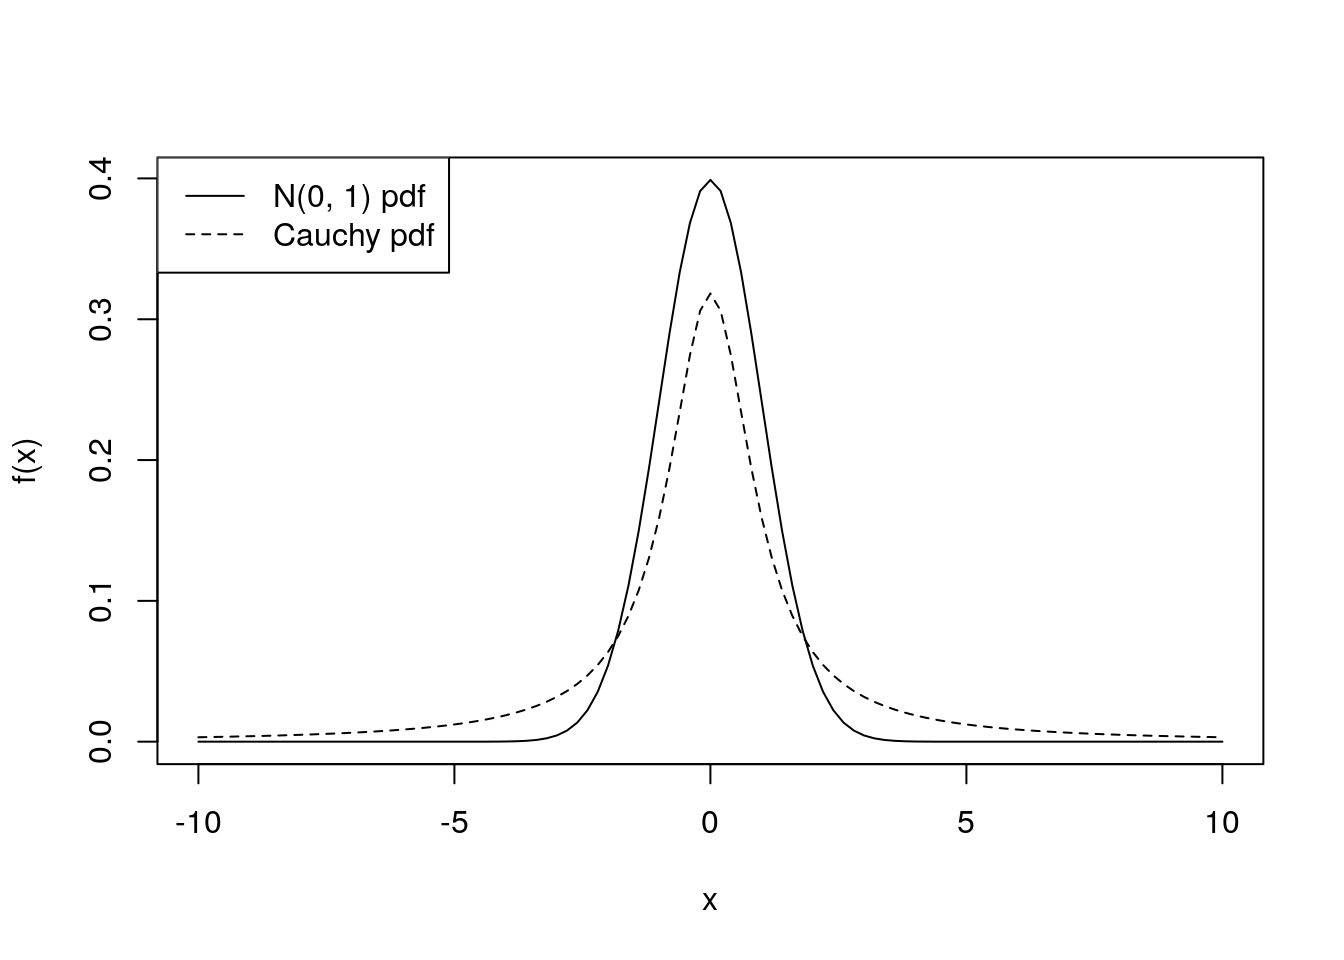
\includegraphics{MATH2011_files/figure-latex/unnamed-chunk-77-1.pdf}

We obtain the Cauchy distribution as the ratio of standard normal random
variables:

\BeginKnitrBlock{proposition}
\protect\hypertarget{prp:unnamed-chunk-78}{}{\label{prp:unnamed-chunk-78}
}Suppose that \(Y_1 \sim N(0, 1)\) and \(Y_2 \sim N(0, 1)\) are
independent standard normal random variables. Then \(U_1 = Y_1 / Y_2\)
has Cauchy distribution.
\EndKnitrBlock{proposition} \BeginKnitrBlock{proof}

\iffalse{} {Proof. } \fi{}Again, in order to use Theorem
\ref{thm:bvtrans} to show this, we need to first define a second random
variable \(U_2\). We will choose \(U_2 = Y_2\).

By independence, the joint pdf of \(Y_1\) and \(Y_2\) is

\begin{align*}
f(y_1, y_2) &= \frac{1}{\sqrt{2 \pi}} \exp\left(-\frac{y_1^2}{2}\right)
  \frac{1}{\sqrt{2 \pi}} \exp\left(-\frac{y_2^2}{2}\right) \\
  &= \frac{1}{2 \pi} \exp \left(-\frac{y_1^2 + y_2^2}{2} \right),
  \quad y_1, y_2 \in \mathbb{R}.
\end{align*}

The inverse transformations are \[Y_1 = U_1 U_2, \quad Y_2 = U_2,\] and
the \(U_1\) and \(U_2\) is clearly \(U_1 \in \mathbb{R}\),
\(U_2 \in \mathbb{R}\).

The Jacobian matrix is \[\bm J = \begin{pmatrix}
  u_2 & * \\
  0 & 1
  \end{pmatrix},\] where we do not need to evaluate the top right entry
marked \(*\), because it will not affect the determinant of \(\bm J\).
So \(\det(\bm J) = u_2\).

So the joint pdf of \(U_1\) and \(U_2\) is

\begin{align*}
g(u_1, u_2) &= \frac{1}{2 \pi} \exp \left(-\frac{u_1^2 u_2^2 + u_2^2}{2} \right) 
\cdot |u_2| \\
&= \frac{|u_2|}{2 \pi} \exp \left(-\frac{u_2^2(1 + u_2^2)}{2} \right) 
\end{align*}

for \(u_1, u_2 \in \mathbb{R}\).

We integrate out \(u_2\) in order to obtain the marginal pdf of \(U_1\)

\begin{align*}
g_1(u_1) &= \int_{-\infty}^\infty g(u_1, u_2) du_2 \\
&= \frac{1}{2 \pi}  \int_{-\infty}^\infty |u_2| \exp \left(-\frac{u_2^2(1 + u_2^2)}{2} \right)  du_2 \\
&= 2 \times \frac{1}{2 \pi} 
\int_{0}^\infty u_2 \exp \left(-\frac{c u_2^2}{2} \right)  du_2,  \; \text{with $c = 1 + u_1^2$} \\
&= \frac{1}{\pi} \left[-\frac{1}{c} \exp\left(-\frac{c u_2^2}{2}\right)\right]_0^\infty \\
&= \frac{1}{\pi} \cdot \frac{1}{c} \\
&= \frac{1}{\pi (1 + u_1)^2}, \quad u_1 \in \mathbb{R},
\end{align*}

which is the Cauchy pdf, so \(U_1\) has Cauchy distribution, as
required.
\EndKnitrBlock{proof}

\section{\texorpdfstring{The \(t\)
distribution}{The t distribution}}\label{the-t-distribution}

\BeginKnitrBlock{definition}
\protect\hypertarget{def:unnamed-chunk-80}{}{\label{def:unnamed-chunk-80} }A
random variable \(Y\) has \(t\) distribution with \(k\) degrees of
freedom if it has pdf \[f(y) = \frac{1}
{\sqrt{k} B\left(\frac{1}{2}, \frac{k}{2}\right)}
\left(1 + \frac{y^2}{k} \right)^{-\frac{k+1}{2}}
, \quad y \in \mathbb{R}.\] We write \(Y \sim t_k\).
\EndKnitrBlock{definition} We can plot the pdfs of the \(t\)
distribution with \(2\), and \(5\) degrees of freedom, compared with the
\(N(0, 1)\) pdf.

\begin{Shaded}
\begin{Highlighting}[]
\KeywordTok{curve}\NormalTok{(}\KeywordTok{dnorm}\NormalTok{(x), }\DataTypeTok{from =} \DecValTok{-5}\NormalTok{, }\DataTypeTok{to =} \DecValTok{5}\NormalTok{, }\DataTypeTok{xlab =} \StringTok{"x"}\NormalTok{, }\DataTypeTok{ylab =} \StringTok{"f(x)"}\NormalTok{)}
\KeywordTok{curve}\NormalTok{(}\KeywordTok{dt}\NormalTok{(x, }\DataTypeTok{df =} \DecValTok{2}\NormalTok{), }\DataTypeTok{add =} \OtherTok{TRUE}\NormalTok{, }\DataTypeTok{lty =} \DecValTok{2}\NormalTok{)}
\KeywordTok{curve}\NormalTok{(}\KeywordTok{dt}\NormalTok{(x, }\DataTypeTok{df =} \DecValTok{5}\NormalTok{), }\DataTypeTok{add =} \OtherTok{TRUE}\NormalTok{, }\DataTypeTok{lty =} \DecValTok{3}\NormalTok{)}
\KeywordTok{legend}\NormalTok{(}\StringTok{"topleft"}\NormalTok{, }\DataTypeTok{lty =} \KeywordTok{c}\NormalTok{(}\DecValTok{1}\NormalTok{, }\DecValTok{2}\NormalTok{, }\DecValTok{3}\NormalTok{),}
       \DataTypeTok{legend =} \KeywordTok{c}\NormalTok{(}\StringTok{"N(0, 1) pdf"}\NormalTok{, }\StringTok{"t_2 pdf"}\NormalTok{, }\StringTok{"t_5 pdf"}\NormalTok{))}
\end{Highlighting}
\end{Shaded}

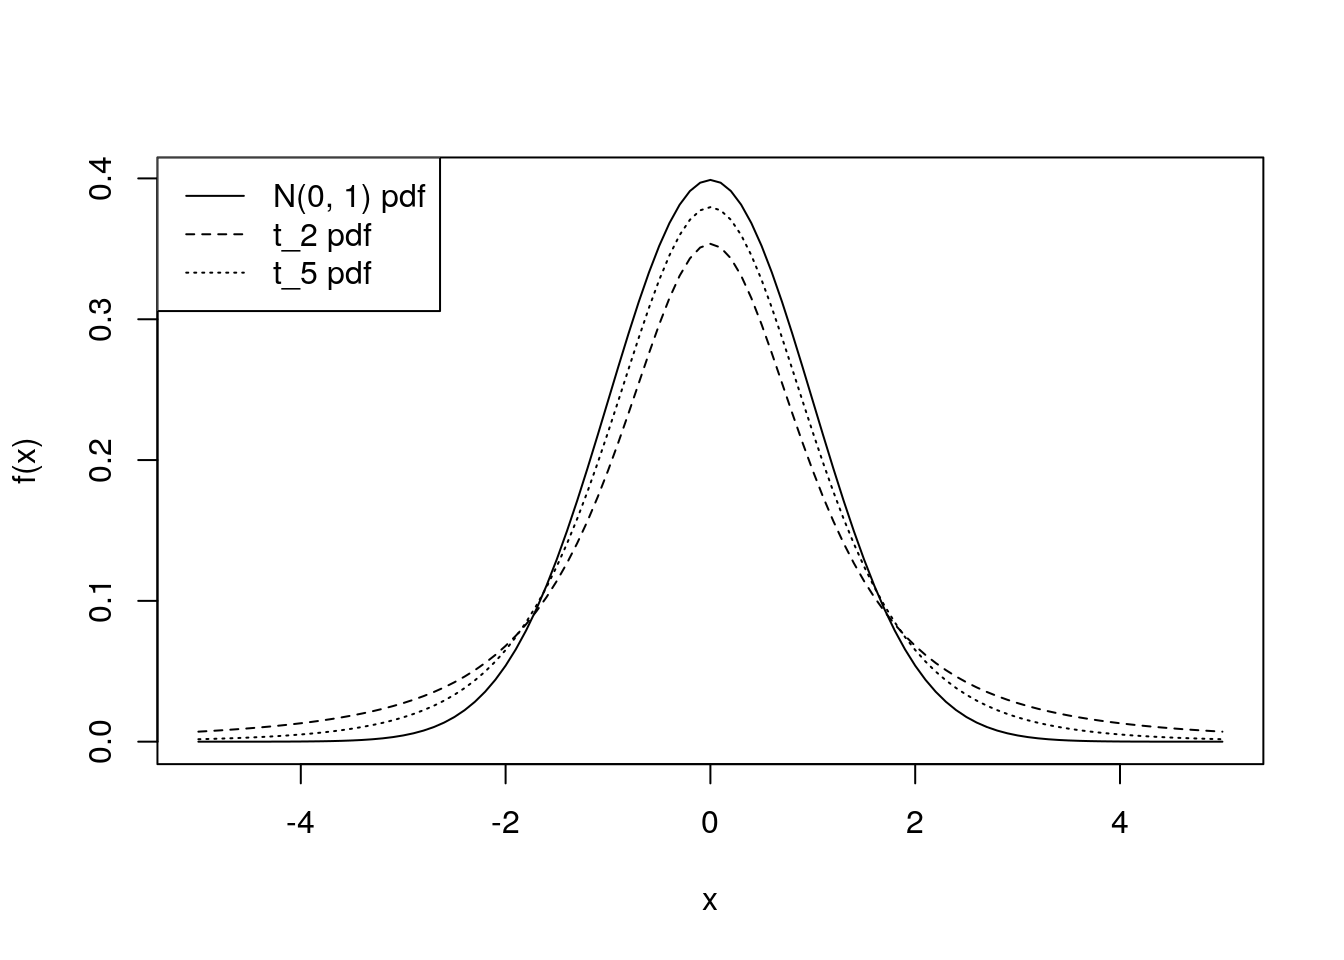
\includegraphics{MATH2011_files/figure-latex/unnamed-chunk-81-1.pdf}

The \(t_k\) distribution has heavier tails than the \(N(0, 1)\)
distribution, but as \(k \rightarrow \infty\),
\(t_k \rightarrow N(0, 1)\). When \(k=1\), the \(t_1\) distribution is
the Cauchy distribution.

We obtain the \(t\) distribution as a ratio of a standard normal random
variable, and a the square root of a chi-squared random variable divided
by its degrees of freedom. Although this sounds complicated, this makes
the \(t\) distribution important in practice, as we will soon see.

\BeginKnitrBlock{proposition}
\protect\hypertarget{prp:tconstruct}{}{\label{prp:tconstruct} }Suppose that
\(Y_1 \sim N(0, 1)\) and \(Y_2 \sim \chi^2_k\), and that \(Y_1\) and
\(Y_2\) are independent. Then
\[U_1 = \frac{Y_1}{\sqrt{Y_k/k}} \sim t_k.\]
\EndKnitrBlock{proposition} \BeginKnitrBlock{proof}

\iffalse{} {Proof. } \fi{}In order to use Theorem \ref{thm:bvtrans} to
show this, we need to first define a second random variable \(U_2\). We
will choose \(U_2 = Y_2\).

The pdfs of \(Y_1\) and \(Y_2\) are
\[f_1(y_1) = \frac{1}{\sqrt{2 \pi}} \exp\left(\frac{-y_1^2}{2} \right),
  \quad y_1 \in \mathbb{R}\] and
\[f_2(y_2) = \frac{y_2^{k/2 - 1}}{\Gamma(k/2) 2^{k/2}} \exp\left(\frac{-y_2}{2}\right),
  \quad y_2 > 0.\] So, by independence, the joint pdf of \(Y_1\) and
\(Y_2\) is
\[f(y_1, y_2) =  \frac{1}{\sqrt{2 \pi}} \exp\Big(\frac{-y_1^2}{2} \Big)
  \frac{y_2^{k/2 - 1}}{\Gamma(k/2) 2^{k/2}} \exp\left(\frac{-y_2}{2}\right),
  \quad y_1 \in \mathbb{R}, y_2 > 0.\]

The inverse transformations are
\[Y_1 = U_1 \sqrt{\frac{U_2}{k}}, \quad Y_2 = U_2,\] and the domain of
\(U_1\) and \(U_2\) is \(U_2 \in \mathbb{R}\), \(U_2 > 0\).

The Jacobian is \[\bm J = \begin{pmatrix}
\sqrt{\frac{u_2}{k}} & * \\
0 & 1
\end{pmatrix},
\] so \(\det \bm J = \sqrt{u_2/k} > 0\).

So the joint pdf of \(U_1\) and \(U_2\) is

\begin{align*}
g(u_1, u_2) &=  \frac{1}{\sqrt{2 \pi}} \exp\Big(-\frac{u_1^2 u_2}{2 k} \Big)
  \frac{y_2^{k/2 - 1}}{\Gamma(k/2) 2^{k/2}} \exp\Big(-\frac{u_2}{2}\Big) \sqrt{\frac{u_2}{k}} \\
    &= \frac{{u_2}^{(k-1)/2}}{2^{(k+1)/2}\sqrt{\pi} \, \Gamma(k/2) \sqrt{k}}
    \exp\Big\{-\frac{u_2}{2} \Big(\frac{u_1^2}{k} + 1 \Big)\Big\}, \quad u_1 \in \mathbb{R},
  u_2 >0.
  \end{align*}

We are interested in the marginal pdf of \(U_1\): \[g_1(u_1) = 
\frac{1}{2^{(k+1)/2}\sqrt{\pi} \, \Gamma(k/2) \sqrt{k}}
\int_0^\infty
    {u_2}^{(k-1)/2} \exp\Big\{-\frac{u_2}{2}
    \Big(\frac{u_1^2}{k} + 1 \Big)
    \Big\} du_2.\] The integrand is proportional to a
\(\text{gamma}(\alpha, \beta)\) pdf
\[h(u_2) = \frac{\beta^\alpha}{\Gamma(\alpha)} u_2^{\alpha - 1}
e^{-\beta u_2}, \quad u_2 > 0, \] if we take \(\alpha = \frac{k+1}{2}\)
and \(\beta = \frac{1}{2}\Big(\frac{u_1^2}{k} + 1\Big)\). So
\[g_1(u_1) = \frac{1}{2^{(k+1)/2}\sqrt{\pi} \, \Gamma(k/2) \sqrt{k}}
\frac{\Gamma((k+1)/2)}{
\left[\frac{1}{2}\big(\frac{u_1^2}{k} + 1\big)\right]^{(k+1)/2}}
\int_0^\infty h(u_2) du_2.\] But \(\int_0^\infty h(u_2) du_2 = 1\) and
\(\sqrt{\pi} = \Gamma(1/2)\), so

\begin{align*}
g_1(u_1) &= \frac{\Gamma(\frac{k+1}{2})}{\Gamma(\frac{k}{2}) \Gamma(\frac{1}{2})}
\frac{\big(1 + \frac{u_1^2}{k} \big)^{-\frac{k+1}{2}}}
{\sqrt{k}} \\
&= \frac{1}{\sqrt{k} B\left(\frac{k}{2}, \frac{1}{2}\right)}
\Big(1 + \frac{u_1^2}{k} \Big)^{-\frac{k+1}{2}}
, \quad u_1 > 0,
\end{align*}

which is the pdf of a \(t_k\) distribution, so \(U_1 \sim t_k\).
\EndKnitrBlock{proof}

The importance of the \(t\) distribution in practice comes from the
following proposition, which we will use to construct confidence
interval and hypothesis tests for the mean of normal random variables in
Chapter \ref{inference}:

\BeginKnitrBlock{proposition}
\protect\hypertarget{prp:ybart}{}{\label{prp:ybart} }Suppose that
\(Y_1, Y_2, \ldots, Y_n\), are independent and identically distributed,
with each \(Y_i \sim N(0, 1)\). Let \(\bar Y\) and \(S^2\) be the usual
sample mean and sample variance. Then
\[\frac{\sqrt{n}(\bar Y - \mu)}{S} \sim t_{n-1}.\]
\EndKnitrBlock{proposition}

\BeginKnitrBlock{proof}
\iffalse{} {Proof. } \fi{}We know from Proposition \ref{prp:ybarnormal}
that \(\bar Y \sim N(\mu, \sigma^2/n)\), so
\[A = \frac{\sqrt{n}(\bar Y - \mu)}{\sigma} \sim N(0, 1).\] We also know
from Theorem \ref{thm:S2dist} that
\[B = \frac{(n - 1) S^2}{\sigma^2} \sim \chi^2_{n-1}.\] So, by
Proposition \ref{prp:tconstruct},
\[\frac{A}{\sqrt{B/(n-1)}} \sim t_{n-1}.\] Simplifying,

\begin{align*}
\frac{A}{\sqrt{B/(n-1)}} &=  A \sqrt{n-1} \frac{1}{\sqrt{B}} \\
&= \frac{\sqrt{n}(\bar Y - \mu)}{\sigma} \sqrt{n-1} \frac{\sigma}{\sqrt{n-1} S} \\
&= \frac{\sqrt{n}(\bar Y - \mu)}{S},
\end{align*}

so \[\frac{\sqrt{n}(\bar Y - \mu)}{S} \sim t_{n-1}\] as required.
\EndKnitrBlock{proof}

\section{\texorpdfstring{The \(F\)
distribution}{The F distribution}}\label{the-f-distribution}

\BeginKnitrBlock{definition}
\protect\hypertarget{def:unnamed-chunk-84}{}{\label{def:unnamed-chunk-84} }A
random variable \(Y\) has \(F\) distribution with \(m\) and \(n\)
degrees of freedom if it has pdf
\[f(y) = \frac{m^{\frac{n}{2}} n^{\frac{m}{2}}}
{B\left(\frac{m}{2}, \frac{n}{2}\right)} 
\frac{y^{\frac{m}{2} - 1}}{(n + my)^{\frac{m + n}{2}}}, \quad y > 0.\]
We write \(Y \sim F_{m, n}\).
\EndKnitrBlock{definition}

We may obtain the \(F\) distribution as the ratio of two independent
chi-squared random variables, each divided by their degrees of freedom.
As with the \(t\) distribution, this makes the \(F\) distribution
important in statistics: \BeginKnitrBlock{proposition}

\protect\hypertarget{prp:fconstruct}{}{\label{prp:fconstruct} }Suppose that
\(Y_1 \sim \chi^2_m\) and \(Y_2 \sim \chi^2_n\), and that \(Y_1\) and
\(Y_2\) are independent. Then
\[U_1 = \frac{Y_1 / m}{Y_2 / n} \sim F_{m, n}.\]
\EndKnitrBlock{proposition}

\BeginKnitrBlock{proof}
\iffalse{} {Proof. } \fi{}Write \(Y_1^* = \frac{Y_1}{m}\) and
\(Y_2^* = \frac{Y_2}{n}\), so \(U_1 = Y_1^*/Y_2^*\). In order to use
Theorem \ref{thm:bvtrans}, we first need to define a second random
variable \(U_2\). We will choose \(U_2 = Y_2^*\).

We have \(Y_1 \sim \chi^2_m \equiv \text{gamma}(m/2, 1/2)\), so by
Proposition \ref{prp:gammascale} (with b = \(1/m\))
\[Y_1^* = \frac{Y_1}{m} \sim \text{gamma}(m/2, m/2).\] Similarly,
\(Y_2^* \sim \text{gamma}(n/2, n/2)\). So the joint pdf of \(Y_1^*\) and
\(Y_2^*\) is \[f(y_1^*, y_2^*) = 
\frac{(\frac{m}{2})^{m/2}}{\Gamma\left(\frac{m}{2}\right)} 
(y_1^*)^{\frac{m}{2}- 1} e^{-\frac{m}{2} y_1^*} \cdot
\frac{(\frac{n}{2})^{n/2}}{\Gamma\left(\frac{n}{2}\right)} 
(y_2^*)^{\frac{n}{2}- 1} e^{-\frac{n}{2} y_2^*}\] for \(y_1^* > 0\),
\(y_2^* > 0\).

The inverse transformation is \(Y_1^* = U_1 U_2\), \(Y_2^* = U_2\). The
domain of \(U_1\) and \(U_2\) is \(U_1 > 0\), \(U_2 > 0\). The Jacobian
is \[\bm J = \begin{pmatrix}
u_2 & * \\
0 & 1 
\end{pmatrix},\] so \(\det{\bm J} = u_2 > 0\). So the joint pdf of
\(U_1\) and \(U_2\) is

\begin{align*}
g(u_1, u_2) &= \frac{(\frac{m}{2})^{m/2}}{\Gamma\left(\frac{m}{2}\right)} 
(u_1 u_2)^{\frac{m}{2}- 1} e^{-\frac{m}{2} u_1 u_2} \cdot
\frac{(\frac{n}{2})^{n/2}}{\Gamma\left(\frac{n}{2}\right)} 
u_2^{\frac{n}{2}- 1} e^{-\frac{n}{2} u_2} \cdot u_2 \\
&= \frac{m^\frac{m}{2} n^\frac{n}{2}}
{\Gamma\left(\frac{m}{2}\right)\Gamma\left(\frac{n}{2}\right)
2^{(m+n)/2}} u_1^{\frac{m}{2}- 1} u_2^{\frac{m+n}{2}- 1}
e^{-\frac{1}{2}(n + mu_1) u_2},
\end{align*}

for \(u_1 > 0\), \(u_2 > 0\).

The marginal pdf of \(U_1\) is
\[g_1(u_1) = \frac{m^\frac{m}{2} n^\frac{n}{2}}
{\Gamma\left(\frac{m}{2}\right)\Gamma\left(\frac{n}{2}\right)
2^{(m+n)/2}} u_1^{\frac{m}{2}- 1}
\int_0^\infty u_2^{\frac{m+n}{2}- 1}
e^{-\frac{1}{2}(n + mu_1) u_2} du_2.\] The integrand is proportional to
a \(\text{gamma}(\alpha, \beta)\) pdf, with \(\alpha = \frac{m+n}{2}\)
and \(\beta = \frac{1}{2}(n + mu_1)\):
\[h(u_2) = \frac{\left[\frac{1}{2}(n + mu_1)\right]^{\frac{m+n}{2}}}
{\Gamma\left(\frac{m+n}{2}\right)}  u_2^{\frac{m+n}{2}- 1}
e^{-\frac{1}{2}(n + mu_1) u_2}\] so we have

\begin{align*}
g_1(u_1) &= \frac{m^\frac{m}{2} n^\frac{n}{2}}
{\Gamma\left(\frac{m}{2}\right)\Gamma\left(\frac{n}{2}\right)
2^{(m+n)/2}} u_1^{\frac{m}{2}- 1} 
\frac{\Gamma\left(\frac{m+n}{2}\right)}
{\left[\frac{1}{2}(n + mu_1)\right]^{\frac{m+n}{2}}}
\int_0^\infty h(u_2) du_2 \\
&= \frac{m^\frac{m}{2} n^\frac{n}{2} \Gamma\left(\frac{m+n}{2}\right)}
{\Gamma\left(\frac{m}{2}\right)\Gamma\left(\frac{n}{2}\right)
}\frac{u_1^{\frac{m}{2}- 1}}{(n + mu_1)^{\frac{m+n}{2}}} \\
&= \frac{m^\frac{m}{2} n^\frac{n}{2}}
{B\left(\frac{m}{2}, \frac{n}{2}\right)}
\frac{u_1^{\frac{m}{2}- 1}}{(n + mu_1)^{\frac{m+n}{2}}},
\quad u_1 > 0,
\end{align*}

which is the pdf of a \(F_{m, n}\) distribution, so
\(U_1 \sim F_{m, n}\).
\EndKnitrBlock{proof}

The importance of the \(F\) distribution in practice comes from the
following proposition, which we will use in Chapter \ref{inference} to
test whether two sets of normal random variables have the same variance:
\BeginKnitrBlock{proposition}
\protect\hypertarget{prp:ftest}{}{\label{prp:ftest} }Suppose
\(Y^{(1)}_1, \ldots, Y^{(1)}_m\) and \(Y^{(2)}_1, \ldots, Y^{(2)}_n\)
are two sets of independent random variables, with each
\(Y^{(1)}_i \sim N(\mu_1, \sigma^2)\) and each
\(Y^{(2)}_i \sim N(\mu_2, \sigma^2)\). Let \(S_1^2\) be the sample
variance of \(Y^{(1)}_1, \ldots, Y^{(1)}_m\) and \(S_2^2\) be the sample
variance of \(Y^{(2)}_1, \ldots, Y^{(2)}_n\). Then
\[\frac{S_1^2}{S_2^2} \sim F_{m-1, n-1}.\]
\EndKnitrBlock{proposition}

\BeginKnitrBlock{proof}
\iffalse{} {Proof. } \fi{}We know from Theorem \ref{thm:S2dist} that
that \((m-1) S_1^2/ \sigma^2 \sim \chi^2_{m-1}\) and
\((n-1) S_2^2 / \sigma^2 \sim \chi^2_{n-1}\), and \(S_1^2\) and
\(S_2^2\) are independent. So by Proposition \ref{prp:fconstruct}
\[\frac{S_1^2 / \sigma^2}{S_2^2 / \sigma^2}
= \frac{S_1^2}{S_2^2} \sim F_{m-1, n-1}\] as required.
\EndKnitrBlock{proof}

\part{Statistical
inference}\label{part-statistical-inference}

\chapter{Parameter estimation}\label{estimation}

\section{Estimators and estimates}\label{estimators-and-estimates}

Suppose that \(Y_1, \ldots, Y_n\) are independent identically
distributed random variables, each with a distribution depending on
unknown parameter(s) \(\theta\). In the continuous case, we know the
density function \(f(y_i; \theta)\) up to the unknown \(\theta\), and in
the discrete case we have probability function \(p(y_i; \theta)\). We
might be interested in estimating \(\theta\) based on
\(Y_1, \ldots, Y_n\).

An \emph{estimator} \(T = T(Y_1, ...,Y_n)\) is just some suitable
function (a ``statistic'') of \(Y_1, Y_2, \ldots, Y_n\), which is used
to estimate a parameter. It must not contain any unknown parameters or
any unobservable quantities. For example, the sample mean \(\bar Y\) is
an obvious estimator for the population mean.

Note that an estimator is a function of random variables and hence can
itself be treated as a random variable. Once a set of data has been
collected (i.e.~the observed values \(y_1, y_2, \ldots ,y_n\) of
\(Y_1, Y_2, \ldots, Y_n\) are available), then \(T(y_1, ...,y_n)\) is
the corresponding \emph{estimate}. When deriving properties of \(T\),
one should always work with the estimator.

You have already seen several desirable properties of estimators in
MATH1024, which we now review.

\section{Bias}\label{bias}

\BeginKnitrBlock{definition}
\protect\hypertarget{def:unnamed-chunk-87}{}{\label{def:unnamed-chunk-87}
}The \emph{bias} of an estimator \(T = T(Y_1, \ldots, Y_n)\) of a
parameter \(\theta\) is: \[B(T; \theta) = E(T) - \theta.\] \(T\) is said
to be an \emph{unbiased} estimator of \(\theta\) if
\[E(T) - \theta = 0\] for all possible values of \(\theta\).
\EndKnitrBlock{definition}

\BeginKnitrBlock{example}[Bias of estimator of Bernoulli success probability]
\protect\hypertarget{exm:bernbias}{}{\label{exm:bernbias} \iffalse (Bias of
estimator of Bernoulli success probability) \fi{} }Let
\(Y_1, Y_2, \ldots, Y_n\) be independent and identically distributed,
where each \(Y_i \sim \text{Bernoulli}(\theta)\).

We know that \(E(Y_i) = \theta\), so a natural estimator of \(\theta\)
is \(T = \bar Y = \frac{1}{n} \sum_{i=1}^n Y_i\), the sample mean.

Here \(T\) is an unbiased estimator of \(\theta\), as
\[E(T) = E(\bar Y) = \frac{1}{n} \sum_{i=1}^n E(Y_i) = \frac{1}{n} n \theta = \theta.\]
\EndKnitrBlock{example}

\BeginKnitrBlock{example}[Bias of estimator of exponential rate parameter]
\protect\hypertarget{exm:expbias}{}{\label{exm:expbias} \iffalse (Bias of
estimator of exponential rate parameter) \fi{} }Let
\(Y_1, Y_2, \ldots, Y_n\) be independent and identically distributed,
where each \(Y_i \sim \text{exponential}(\theta)\).

We know that \(E(Y_i) = 1/\theta,\) so one possible estimator for
\(\theta\) is \(T = 1 / \bar Y\).

Since \(Y_i \sim \text{gamma}(1, \theta)\), by Propositions
\ref{prp:gammascale} and \ref{prp:gammasum},
\[\bar Y \sim \text{gamma}(n, n \theta).\]

Recall from Proposition \ref{prp:gammamoments} that
\(E(X) = \alpha/ \beta\) if \(X \sim \text{gamma}(\alpha, \beta)\). So
\(\bar Y\) is an unbiased estimator of \(1/\theta\), as
\[E(\bar Y) = \frac{n}{n \theta} = \frac{1}{\theta}.\]

Given this, an obvious choice for an estimator of \(\theta\) is
\(T = 1 / \bar Y\). Since \(\bar Y \sim \text{gamma}(n, n \theta)\), we
have

\begin{align*}
E(1 / \bar Y) &= \int_0^\infty \frac{1}{y} 
\frac{(n \theta)^n}{\Gamma(n)} y^{n - 1} e^{- n \theta y} dy \\
&= \frac{(n \theta)^n}{\Gamma(n)} \int_0^\infty y^{n-2} e^{- n \theta y} dy \\
&= \frac{(n \theta)^n}{\Gamma(n)} 
\frac{\Gamma(n-1)}{(n \theta)^{n-1}} 
\int_0^\infty \frac{(n \theta)^{n-1}}{\Gamma(n-1)} y^{n-2} e^{- n \theta y} dy \\
&\quad \text{(integrating the $\text{gamma}(n - 1, n \theta)$ pdf)}
\\
&= \frac{\Gamma(n-1)}{\Gamma(n)} n \theta \cdot 1  \\
&= \frac{1}{n-1} n \theta,
\end{align*}

since \(\Gamma(n) = (n-1) \Gamma(n - 1)\), by Proposition
\ref{prp:gammarecursion}. So the bias of \(1/\bar Y\) as an estimator of
\(\theta\) is \[B(1/\bar Y; \theta) = \frac{n}{n-1} \theta - \theta
= \frac{1}{n-1} \theta \not = 0.\] \(1/\bar Y\) is not an unbiased
estimator of \(\theta\), but the bias shrinks with \(n\).
\EndKnitrBlock{example}

\section{Consistency}\label{consistency}

\BeginKnitrBlock{definition}
\protect\hypertarget{def:unnamed-chunk-88}{}{\label{def:unnamed-chunk-88}
}An estimator \(T = T(Y_1, \ldots,Y_n)\) of a parameter \(\theta\) is
said to be a \emph{consistent} estimator of \(\theta\) if:

\begin{enumerate}
\def\labelenumi{\arabic{enumi}.}
\tightlist
\item
  it is \emph{asymptotically unbiased}: \(B(T; \theta) \rightarrow 0\)
  as \(n \rightarrow \infty\); and
\item
  \(\text{Var}(T) \rightarrow 0\) as \(n \rightarrow \infty\).
\end{enumerate}

for all possible values of \(\theta\).
\EndKnitrBlock{definition}

Note that a consistent estimator can be biased, and an unbiased
estimator can be inconsistent (i.e.~not consistent). So consistency and
unbiasedness are different types of property.

\BeginKnitrBlock{example}[Consistency of estimator of Bernoulli success probability]
\protect\hypertarget{exm:bernconsist}{}{\label{exm:bernconsist}
\iffalse (Consistency of estimator of Bernoulli success probability)
\fi{} }Continue example \ref{exm:bernbias}, with
\(Y_i \sim \text{Bernoulli}(\theta)\) and \(T = \bar Y\). \(T\) is a
consistent estimator of \(\theta\), as:

\begin{enumerate}
\def\labelenumi{\arabic{enumi}.}
\tightlist
\item
  \(E(T) = E(\bar Y) = \theta\), so \(B(T; \theta) = 0\). Therefore
  \(B(T; \theta) \rightarrow 0\) as \(n \rightarrow \infty\) (any
  unbiased estimator is asymptotically unbiased).
\item
  The variance is

  \begin{align*}
  \text{Var}(T) &= \text{Var}(\bar Y) 
  = \text{Var}\left(\frac{1}{n} \sum_{i=1}^n Y_i \right) \\
  &= \frac{1}{n^2} \sum_{i=1}^n \text{Var}(Y_i) \quad
  \text{by independence} \\
  &= \frac{1}{n^2} n \theta (1 - \theta) \\
  &\rightarrow 0 \quad \text{as $n \rightarrow \infty$,
  for all $\theta \in [0, 1]$.}
  \end{align*}
\end{enumerate}
\EndKnitrBlock{example}

\BeginKnitrBlock{example}[Consistency of estimator of exponential rate parameter]
\protect\hypertarget{exm:unnamed-chunk-89}{}{\label{exm:unnamed-chunk-89}
\iffalse (Consistency of estimator of exponential rate parameter) \fi{}
}Continue example \ref{exm:expbias}, with
\(Y_i \sim \text{exponential}(\theta)\) and \(T = \frac{1}{\bar Y}\).
\(T\) is a consistent estimator of \(\theta\), as:

\begin{enumerate}
\def\labelenumi{\arabic{enumi}.}
\tightlist
\item
  The bias of \(T\) is
  \[B(T; \theta) = \frac{1}{n-1} \theta \rightarrow 0\] as
  \(n \rightarrow \infty\).
\item
  The variance of \(T\) is \(\text{Var}(T) = E(T^2) - [E(T)]^{2}\).
  Recall \(\bar Y \sim \text{gamma}(n, n \theta)\), so

  \begin{align*}
  E(T^2) &= E({\bar Y}^{-2})
  = \int_0^\infty \frac{1}{y^2} 
  \frac{(n \theta)^n}{\Gamma(n)} y^{n - 1} e^{- n \theta y} dy \\  &= \frac{(n \theta)^n}{\Gamma(n)} \int_0^\infty y^{n-3} e^{- n \theta y} dy \\
  &= \frac{(n \theta)^n}{\Gamma(n)} 
  \frac{\Gamma(n-2)}{(n \theta)^{n-2}} 
  \int_0^\infty \frac{(n \theta)^{n-2}}{\Gamma(n-2)} y^{n-3} e^{- n \theta y} dy \\
  &\quad \text{(integrating the $\text{gamma}(n - 2, n \theta)$ pdf)}
  \\
  &= \frac{\Gamma(n-2)}{\Gamma(n)} (n \theta)^2 \cdot 1  \\
  &= \frac{1}{(n-1)(n-2)} (n \theta)^2,
  \end{align*}

  since \(\Gamma(n) = (n-1) \Gamma(n - 1) = (n-1) (n-2) \Gamma(n-2)\),
  by Proposition \ref{prp:gammarecursion}. So

  \begin{align*}
  \text{Var}(T) &= E(T^2) - [E(T)]^{2} \\
  &= \frac{1}{(n-1)(n-2)} (n \theta)^2 - \frac{1}{(n-1)^2} (n \theta)^2 \\ 
  &= \frac{(n \theta)^2}{(n-1)^2} \left[\frac{n-1}{n-2} - 1 \right] \\
  &\rightarrow 0 \quad \text{as $n \rightarrow \infty$,
  for all $\theta>0$.}
  \end{align*}
\end{enumerate}
\EndKnitrBlock{example}

\section{Mean squared error}\label{mean-squared-error}

If we have two unbiased estimators, \(T_1\) and \(T_2\), of \(\theta\)
then typically we prefer the one with the smaller variance. However,
having a small variance on its own is not sufficient if the estimator is
biased.

\BeginKnitrBlock{definition}
\protect\hypertarget{def:unnamed-chunk-90}{}{\label{def:unnamed-chunk-90}
}The \emph{mean squared error} (or \emph{MSE}) of an estimator \(T\) of
\(\theta\) is \[\text{MSE}(T; \theta) = E\{(T - \theta)^2\},\] the mean
of the squared distance of the \(T\) from its target value \(\theta.\)
\EndKnitrBlock{definition}

We can use the MSE to choose between competing estimators whether they
are unbiased or not.

\BeginKnitrBlock{proposition}
\protect\hypertarget{prp:biasvardecomp}{}{\label{prp:biasvardecomp} }For any
estimator \(T\) of \(\theta\),
\[\text{MSE}(T; \theta) = \text{Var}(T) + \left[B(T; \theta)\right]^2.\]
\EndKnitrBlock{proposition} \BeginKnitrBlock{proof}

\iffalse{} {Proof. } \fi{}We have

\begin{align*}
\text{MSE}(T; \theta) &= E\{(T - \theta)^2\} \\
&= E\{(T - E(T) + E(T) - \theta)^2\}  \\
&= E\left\{(T - E(T))^2 + 2(T - E(T))(E(T) - \theta)
+ (E(T) - \theta)^2 \right\} \\
&= E\left\{(T - E(T))^2 \right\} + 2(E(T) - \theta) 
E\left\{T - E(T) \right\} +(E(T) - \theta)^2 \\
&= \text{Var}(T) + 2(E(T) - \theta) \cdot 0 + \left[B(T; \theta)\right]^2 \\
&= \text{Var}(T) + \left[B(T; \theta)\right]^2,
\end{align*}

as required.
\EndKnitrBlock{proof}

An immediate consequence of Proposition \ref{prp:biasvardecomp} is that
if \(T\) is an unbiased estimator of \(\theta\), then
\(\text{MSE}(T; \theta) = \text{Var}(T)\).

Note that it is not possible to find a \emph{uniformly} minimum MSE
estimator, that is, an estimator which will have the lower MSE than any
other estimator for all value of \(\theta\). For instance, consider the
estimator \(T^* = 1\), which takes the simple (but usually bad!)
strategy of estimating \(\theta\) as \(1\), irrespective of the observed
data. This has \textbf{zero} mean squared error at \(\theta = 1\), so
will beat any other estimator at \(\theta = 1\). However, it will be a
very bad estimator for other values of \(\theta\).

It is sometimes possible to find a uniformly minimum MSE estimator
within a class of ``sensible'' estimators.

\BeginKnitrBlock{example}[Comparing estimators of the normal variance parameter]
\protect\hypertarget{exm:unnamed-chunk-92}{}{\label{exm:unnamed-chunk-92}
\iffalse (Comparing estimators of the normal variance parameter) \fi{}
}Suppose that \(Y_1, Y_2, \ldots, Y_n\) are independent, with each
\(Y_i \sim N(\mu, \sigma^2)\), and that we wish to estimate
\(\sigma^2\). Two possible choices are:
\(S^2 = \frac{1}{n-1} \sum_{i=1}^n (Y_i - \bar Y)^2\) and
\(\frac{1}{n} \sum_{i=1}^n (Y_i - \bar Y)^2.\) You can think of these as
special cases of estimators of the form
\[T_c = c \sum_{i=1}^n (Y_i - \bar Y)^2,\] where \(c\) is some positive
constant.

Can we find a value of \(c\) such that \(\text{MSE}(T_c; \sigma^2)\) is
minimised for all \(\sigma^2 > 0\)? From Theorem \ref{thm:S2dist},
\(\frac{(n-1) S^2}{\sigma^2} \sim \chi^2_{n-1}\), so
\[\frac{T_c}{c \sigma^2} = \frac{\sum_{i=1}^n (Y_i - \bar Y)^2}{\sigma^2} \sim \chi^2_{n-1}.\]
We may use this to find \(\text{MSE}(T_c; \sigma^2)\) for any \(c\), and
then minimise it with respect to \(c\).

By Proposition \ref{prp:biasvardecomp},
\[\text{MSE}(T_c; \sigma^2) = \text{Var}(T_c) + \left[B(T_c; \sigma^2)\right]^2.\]
Let \(X = \frac{T_c}{c \sigma^2} \sim \chi^2_{n-1}\). Recall from
Section \ref{chisquared} that \(E(X) = n - 1\) and
\(\text{Var}(X) = 2(n-1)\). We have
\[E(T_c) = E(c \sigma^2 X) = c \sigma^2 E(X) = c \sigma^2 (n-1),\] so
\[B(T_c; \sigma^2) = \sigma^2 [c (n-1) - 1] .\] The variance of \(T_c\)
is \[\text{Var}(T_c) = \text{Var}(c \sigma^2 X) 
= c^2 \sigma^4 \text{Var}(X) = c^2 \sigma^4 2(n-1),\] so the mean
squared error is

\begin{align*}
\text{MSE}(T_c; \sigma^2) &= c^2 \sigma^4 2(n-1) + \sigma^4[c (n-1) - 1]^2 \\
&= \sigma^4 \left[2c^2 (n-1) + c^2 (n-1)^2 - 2c(n-1) + 1\right].
\end{align*}

To minimise this, for any \(\sigma^2\), we need to find \(c\) to
minimise \[g(c) = 2c^2 (n-1) + c^2 (n-1)^2 - 2c(n-1) + 1.\]
Differentiating, we have \[g^\prime(c) = 4c(n-1) + 2c(n-1)^2- 2(n-1),\]
so we want to find \(c^*\) such that \(g^\prime(c^*) = 0\), or
\[4c^*(n-1) + 2c^*(n-1)^2- 2(n-1) = 0.\] Dividing by \(2(n - 1)\) and
rearranging gives \(c^*(2 + n-1) = 1,\) so \(c^* = \frac{1}{n+1}\). So
\[T_{c^*} = \frac{1}{n+1} \sum_{i=1}^n (Y_i - \bar Y)^2\] has minimum
mean squared error of all estimators in this class, for any value of
\(\sigma^2\).
\EndKnitrBlock{example}

Once we have come up with an estimator, we can check whether it has good
properties, such as consistency or low mean squared error. However, it
is not yet clear yet how we should go about finding an estimator for any
given model, and it would be useful to have some general methods that
will produce estimators. We will consider two general recipes for
finding estimators, the method of moments, and maximum likelihood
estimation.

\section{Method of moments
estimation}\label{method-of-moments-estimation}

This approach essentially formalises an argument we have met before --
``if I have data from a population with mean \(\mu\), it is natural to
estimate \(\mu\) by the corresponding sample mean \(\bar Y\)''.

Suppose we have a sample of independent and identically distributed
random variables \(Y_1, Y_2, \ldots,Y_n\), whose probability function or
probability density function depends on \(k\) unknown parameters
\((\theta_1, \theta_2, \ldots, \theta_k)\). Then we may write the
\(r\)th population moment about the origin as a function of the
parameters:
\[\mu_r^\prime = \mu_r^\prime(\theta_1, \theta_2, \ldots, \theta_k), \quad \text{for $r = 1, 2, 3, \ldots$.}\]
We write \[m_r^\prime = \frac{1}{n} \sum_{i=1}^n Y_i^r\] for the \(r\)th
sample moment, for \(r = 1, 2, 3, \ldots\).

Then (assuming each of the first \(k\) moments involves at least one
parameter) we find values \(\tilde \theta_1, \ldots, \tilde \theta_k\)
such that the first \(k\) sample moments match the first \(k\)
population moments
\[m_r^\prime = \mu_r^\prime(\tilde \theta_1, \tilde \theta_2, \ldots, \tilde \theta_k) \text{ for $r = 1, 2, \ldots$, k}.\]
We call \(\tilde \theta_1, \ldots, \tilde \theta_k\) the \emph{method of
moments estimators} of of \(\theta_1, \ldots, \theta_k\).

Sometimes one of the first \(k\) expressions does not involve any
parameters, in which case we need to add an extra simultaneous equation
\[m_{k+1}^\prime = \mu_{k+1}^\prime(\tilde \theta_1, \tilde \theta_2, \ldots, \tilde \theta_k)\]
in order to be able to solve the system of simultaneous equations for
the \(k\) unknowns \(\tilde \theta_1, \ldots, \tilde \theta_k\) We
always need at least \(k\) simultaneous equations to solve for the \(k\)
unknowns: if any of those simultaneous equations does not provide any
new information, then we need to generate more equations by matching
higher-order population and sample moments, until it is possible to find
a solution to the system of simultaneous equations.

This will become clearer with some examples. We first begin with some
simple one-parameter examples to illustrate the method.

\BeginKnitrBlock{example}[Bernoulli]
\protect\hypertarget{exm:bernmom}{}{\label{exm:bernmom} \iffalse (Bernoulli)
\fi{} }Suppose \(Y_i \sim \text{Bernoulli}(\theta)\). We have
\(\mu_1^\prime = \mu_1^\prime(\theta) = \theta\). and
\(m_1 = \frac{1}{n}\sum_{i=1}^n Y_i = \bar Y\). So the method of moments
estimator is \(\tilde \theta = \bar Y\).
\EndKnitrBlock{example}

\BeginKnitrBlock{example}[Normal mean]
\protect\hypertarget{exm:unnamed-chunk-93}{}{\label{exm:unnamed-chunk-93}
\iffalse (Normal mean) \fi{} }Suppose \(Y_i \sim N(\theta, 1)\). We have
\(\mu_1^\prime = \mu_1^\prime(\theta) = \theta\), and
\(m_1 = \frac{1}{n}\sum_{i=1}^n Y_i = \bar Y\). So the method of moments
estimator is \(\tilde \theta = \bar Y\).
\EndKnitrBlock{example}

\BeginKnitrBlock{example}[Exponential]
\protect\hypertarget{exm:expmom}{}{\label{exm:expmom} \iffalse (Exponential)
\fi{} }Suppose \(Y_i \sim \text{exponential}(\theta)\). We have
\(\mu_1^\prime = \mu_1^\prime(\theta) = 1/\theta,\) and
\(m_1 = \frac{1}{n}\sum_{i=1}^n Y_i = \bar Y\). So the method of moments
estimator is \(\tilde \theta = 1/ \bar Y\).
\EndKnitrBlock{example}

\BeginKnitrBlock{example}[Normal variance]
\protect\hypertarget{exm:unnamed-chunk-94}{}{\label{exm:unnamed-chunk-94}
\iffalse (Normal variance) \fi{} }Suppose \(Y_i \sim N(0, \theta)\). We
know that \(\mu_1^\prime = \mu_1^\prime(\theta) = 0\), which does not
involve the parameter of interest. But
\(\mu_2^\prime = \mu_2^\prime(\theta) = \theta\), and
\(m_2^\prime = \frac{1}{n}\sum_{i=1}^n Y_i^2,\) so
\(\tilde \theta = \frac{1}{n} \sum_{i=1}^n Y_i^2.\)
\EndKnitrBlock{example}

We can also use method of moment estimation for models with more than
one unknown parameter.

\BeginKnitrBlock{example}[Normal mean and variance]
\protect\hypertarget{exm:unnamed-chunk-95}{}{\label{exm:unnamed-chunk-95}
\iffalse (Normal mean and variance) \fi{} }Suppose
\(Y_i \sim N(\theta_1, \theta_2)\) (i.e. \(\theta_1 = \mu\),
\(\theta_2 = \sigma^2\) in the usual notation). The first two population
moments are \(\mu_1^\prime(\theta_1, \theta_2) = \theta_1\) and
\[\mu_2^\prime(\theta_1, \theta_2) = \text{Var}(Y) + [E(Y)]^2 = \theta_2 + \theta_1^2.\]
The first two sample moments are \(m_1^\prime = \bar Y\) and
\(m_2^\prime = \frac{1}{n}\sum_{i=1}^n Y_i^2\). So we choose
\(\tilde \theta_1\) and \(\tilde \theta_2\) to solve
\(\mu_1^\prime(\tilde \theta_1, \tilde \theta_2) = m_1^\prime\) and
\(\mu_2^\prime(\tilde \theta_1, \tilde \theta_2) = m_2^\prime\). So
\[\tilde \theta_1 = \bar Y \quad \text{and} \quad \tilde \theta_2 + \tilde \theta_1^2 = \frac{1}{n}\sum_{i=1}^n Y_i^2,\]
so \[\tilde \theta_2 = \frac{1}{n}\sum_{i=1}^n Y_i^2 - \bar Y^2.\]
\EndKnitrBlock{example}

\BeginKnitrBlock{example}
\protect\hypertarget{exm:unnamed-chunk-96}{}{\label{exm:unnamed-chunk-96}
}Suppose \(Y_i \sim \text{gamma}(\theta_1, \theta_2)\) In this notation
the shape parameter is \(\alpha = \theta_1\) and the rate parameter is
\(\beta = \theta_2\).

By Proposition \ref{prp:gammamoments}, we have
\[\mu_1^\prime(\theta_1, \theta_2) = \frac{\theta_1}{\theta_2}\] and

\begin{align*}
\mu_2^\prime(\theta_1, \theta_2) &= 
\text{Var}(Y) + [E(Y)]^2 \\
&= \frac{\theta_1}{\theta_2^2} + \frac{\theta_1^2}{\theta_2^2} \\
&= \frac{\theta_1(1 + \theta_1)}{\theta_2^2}.
\end{align*}

The first two sample moments are \(m_1^\prime = \bar Y\) and
\(m_2^\prime = \frac{1}{n}\sum_{i=1}^n Y_i^2\).

So we choose \(\tilde \theta_1\) and \(\tilde \theta_2\) to solve
\(\mu_1^\prime(\tilde \theta_1, \tilde \theta_2) = m_1^\prime\) and
\(\mu_2^\prime(\tilde \theta_1, \tilde \theta_2) = m_2^\prime\). So
\[\frac{\tilde \theta_1}{\tilde \theta_2} = \bar Y
\quad \text{and} \quad
\frac{\tilde \theta_1(1 + \tilde \theta_1)}{\tilde \theta_2^2} = \frac{1}{n}\sum_{i=1}^n Y_i^2.\]
So \(\tilde \theta_1 = \bar Y \tilde \theta_2\), and
\[\frac{\bar Y \tilde \theta_2}{(1 + \bar Y \tilde \theta_2)}{\tilde \theta_2^2} = \frac{1}{n}\sum_{i=1}^n Y_i^2,\]
or
\[\bar Y \tilde{\theta}_2^{-1} + {\bar Y}^2 = \frac{1}{n}\sum_{i=1}^n Y_i^2.\]
Rearranging, we get
\[\tilde \theta_2 = \frac{\bar Y}{\frac{1}{n}\sum_{i=1}^n Y_i^2 - {\bar Y}^2},\]
so
\[\tilde \theta_1 = \bar Y \tilde \theta_2 = \frac{\bar Y^2}{\frac{1}{n}\sum_{i=1}^n Y_i^2 - {\bar Y}^2}.\]
\EndKnitrBlock{example}

\section{Maximum likelihood
estimation}\label{maximum-likelihood-estimation}

Maximum likelihood estimation is a versatile method -- it is the
standard method in modern (frequentist) statistics -- and it can be
shown (see MATH3044) that maximum likelihood estimators (MLEs) have some
nice optimality properties.

Maximum likelihood estimation can be applied in complex situations, but
in this module we will stick to the situation where
\(Y_1, Y_2, \ldots, Y_n\) are independent and identically distributed
random variables,

The likelihood function is a function of the unknown parameters
\(\theta\), which gives the joint probability (or joint probability
density) of seeing the observed data \(y_1, \ldots y_n\), assuming the
data were generating from the model with parameter value \(\theta\):
\BeginKnitrBlock{definition}
\protect\hypertarget{def:unnamed-chunk-97}{}{\label{def:unnamed-chunk-97}
}Suppose \(Y_1, Y_2, \ldots, Y_n\) are independent and identically
distributed random variables, with distribution depending on a vector of
unknown parameters \(\theta\). The \emph{likelihood function} is
\[L(\theta; y_1, \ldots, y_n) = f(y_1 ; \theta) \times f(y_2 ; \theta) \times \ldots \times  f(y_n ; \theta),\]
if each \(Y_i\) has continuous distribution, with probability density
function \(f(y; \theta)\), or
\[L(\theta; y_1, \ldots, y_n) = p(y_1 ; \theta) \times p(y_2 ; \theta) \times \ldots \times p(y_n ; \theta).\]
if each \(Y_i\) has discrete distribution, with probability function
\(p(y; \theta)\).
\EndKnitrBlock{definition}

The values of the observations \(y_1, \ldots, y_n\) have been observed,
so these are known, and \(L(\cdot)\) may be regarded as a function of
the unknown \(\theta\).

If
\(L(\theta_1 ; y_1 , \ldots, y_n) > L(\theta_2 ; y_1 , \ldots, y_n )\),
we should prefer \(\theta_1\) to \(\theta_2\) because there is a greater
likelihood that the observed data would occur with this value of
\(\theta_1\) than with \(\theta_2\). It follows that we should try to
maximise the likelihood to find the value of \(\theta\) which is most
likely to have given rise to the data that were actually observed.

The maximum likelihood estimate
\(\hat \theta = \hat \theta(y_1, \ldots, y_n)\) of \(\theta\). is the
value of \(\theta\) which maximises the likelihood:
\[\hat \theta = \arg \max_{\theta}L(\theta; y_1, \ldots, y_n)\] The
corresponding maximum likelihood estimator is
\(\hat \theta = \hat \theta(Y_1, \ldots, Y_n)\).

Since we assume that the \(Y_i\) are independent and identically
distributed, the likelihood is just a product of pdf or probability
function terms. Maximising a sum is usually easier than maximising a
product, so we often work with the log-likelihood
\[\log L(\theta; y_1, \ldots, y_n) = 
  \sum_{i=1}^n \log f(y_i; \theta).\]

The value of \(\theta\) which maximises \(L(\cdot)\) is the same as that
which maximises \(\log L(\cdot)\), as \(L(\theta_1 ) > L(\theta_2)\) if
and only if \(\log L(\theta_1) > \log L(\theta_2)\). So we may find the
MLE as by maximising \(\log L(\cdot)\):
\[\hat \theta = \arg \max_{\theta}\left\{\log L(\theta; y_1, \ldots, y_n)\right\}.\]

\BeginKnitrBlock{example}[Bernoulli]
\protect\hypertarget{exm:unnamed-chunk-98}{}{\label{exm:unnamed-chunk-98}
\iffalse (Bernoulli) \fi{} }Suppose
\(Y_i \sim \text{Bernoulli}(\theta)\). The likelihood is
\[L(\theta; y_1, \ldots, y_n) = \prod_{i=1}^n p(y_i; \theta)
= \prod_{i=1}^n \theta^{y_i} (1 - \theta)^{1- y_i}.\] Hence the
log-likelihood is

\begin{align*}
\log L(\theta; y_1, \ldots, y_n) &= 
\log\left(\prod_{i=1}^n \theta^{y_i} (1 - \theta)^{1- y_i}\right)\\
&= \sum_{i=1}^n \log\left(\theta^{y_i} (1 - \theta)^{1- y_i}\right) \\
&= \sum_{i=1}^n \log \theta^{y_i} + \log(1 - \theta)^{1-y_i} \\
&=  \sum_{i=1}^n y_i \log \theta + (1 - y_i) \log (1 - \theta) \\
&= \left(\sum_{i=1}^n y_i\right) \log \theta + 
\left(n - \sum_{i=1}^n y_i\right) \log (1 - \theta).
\end{align*}

We now maximise \(\log L(\cdot)\) as a function of \(\theta\). We
attempt to find a stationary point of \(\log L(\cdot)\) by
differentiating and setting to zero. We have
\[\frac{d}{d \theta}\log L(\theta; y_1, \ldots, y_n)
= \frac{\sum_{i=1}^n y_i}{\theta} - 
\frac{n - \sum_{i=1}^n y_i}{1 - \theta},\] and we want to find
\(\hat \theta\) such that
\[\frac{d}{d \theta}\log L(\theta; y_1, \ldots, y_n)|_{\theta = \hat \theta} = 0.\]
We have \[\frac{\sum_{i=1}^n y_i}{\hat \theta} - 
\frac{n - \sum_{i=1}^n y_i}{1 - \hat \theta)} = 0,\] and rearranging
gives that \[\hat \theta = \frac{\sum_{i=1}^n y_i}{n} = \bar y\] is a
stationary point of the log-likelihood, provided that
\(\sum_{i=1}^n y_i > 0\) and \(\sum_{i=1}^n y_i < n\). If
\(\sum_{i=1}^n y_i = 0\), then \(\log L(\theta) = n \log (1 - \theta)\),
which is decreasing with \(\theta\), so \(\hat \theta = 0\) is the MLE.
Similarly, if \(\sum_{i=1}^n y_i = n\), then
\(\log L(\theta) = n \log \theta\), which is increasing with \(\theta\),
so \(\hat \theta = 1\) is the MLE.

If \(0 < \sum_{i=1}^n y_i < n\), we have shown that
\(\hat \theta = \bar y\) is a stationary point of the the
log-likelihood, but we still need to show that it is a maximum. To do
this, we need to show that
\[\frac{d^2}{d\theta^2} \log L(\theta;y_1, \ldots, y_n)|_{\theta = \hat \theta} < 0.\]
We have \[\frac{d^2}{d\theta^2} = -\frac{\sum_{i=1}^n y_i}{\theta^2} - 
\frac{n - \sum_{i=1}^n y_i}{(1 - \theta)^2},\] so
\[\frac{d^2}{d\theta^2} \log L(\theta;y_1, \ldots, y_n)|_{\theta = \hat \theta} = -\frac{\sum_{i=1}^n y_i}{\hat \theta^2} - 
\frac{n - \sum_{i=1}^n y_i}{(1 - \hat \theta)^2}.\] We know
\(\hat \theta = \bar y\), so \(0 < \hat \theta < 1\), as we are
considering the case \(0 < \sum_{i=1}^n y_i < n\). So \(\hat \theta>0\)
and \(1 - \hat \theta > 0\), so
\[\frac{d^2}{d\theta^2} \log L(\theta;y_1, \ldots, y_n)|_{\theta = \hat \theta} < 0,\]
and \(\hat \theta = \bar Y\) is the maximum likelihood estimate.

In this case, the MLE \(\hat \theta\) is the same as the method of
moments estimate \(\tilde \theta\) we found in Example
\ref{exm:bernmom}. We have already studied the properties of this
estimator, so know that \(\hat \theta\) is an unbiased (see Example
\ref{exm:bernbias}) and consistent (see Example \ref{exm:bernconsist})
estimator of \(\theta\).
\EndKnitrBlock{example}

\BeginKnitrBlock{example}[Exponential]
\protect\hypertarget{exm:unnamed-chunk-99}{}{\label{exm:unnamed-chunk-99}
\iffalse (Exponential) \fi{} }Suppose the
\(Y_i \sim \text{exponential}(\theta)\), so that each \(Y_i\) has pdf
\(f(y; \theta) = \theta e^{- \theta y}\) for \(y > 0\).

The likelihood is
\[L(\theta; y_1, \ldots, y_n) = \prod_{i=1}^n f(y_i; \theta)
= \prod_{i=1}^n \theta e^{-\theta y_i},\] since we know \(y_i > 0\) for
all \(i\).

The log-likelihood is

\begin{align*}
\log L(\theta; y_1, \ldots, y_n) 
&= \sum_{i=1}^n \log\left(\theta e^{-\theta y_i}\right) \\
&= \sum_{i=1}^n \left\{\log \theta + \log\left(e^{-\theta y_i}\right) \right\} \\
&= n \log \theta - \theta \sum_{i=1}^n y_i.
\end{align*}

Differentiating, we have
\[\frac{d}{d \theta} \log L(\theta; y_1, \ldots, y_n)
= \frac{n}{\theta} - \sum_{i=1}^n y_i,\] so a stationary point of the
log-likelihood \(\hat \theta\) satisfies
\[\frac{n}{\hat \theta} - \sum_{i=1}^n y_i = 0.\] Rearranging this, we
get \[\hat \theta = \frac{n}{\sum_{i=1}^n y_i} = \frac{1}{\bar y}.\]

Differentiating again, we have
\[\frac{d^2}{d \theta^2} \log L(\theta; y_1, \ldots, y_n) = - \frac{n}{\hat \theta} < 0 \quad \text{for all $\theta$},\]
so \(\hat \theta\) is a maximum of \(\log L(\cdot)\), and hence
\(\hat \theta\) is the MLE.

In this case, the MLE \(\hat \theta\) is the same as the method of
moments estimate \(\tilde \theta\) we found in Example \ref{exm:expmom}.
\EndKnitrBlock{example}

\BeginKnitrBlock{example}[Gamma]
\protect\hypertarget{exm:unnamed-chunk-100}{}{\label{exm:unnamed-chunk-100}
\iffalse (Gamma) \fi{} }Suppose \(Y_i \sim \text{gamma}(\theta, 1)\).

To find the method of moments estimate of \(\theta\), we have
\(\mu_1^\prime = E(Y_i) = \theta\) and \(m_1^\prime = \bar Y\), so
\(\tilde \theta = \bar Y\).

To find the maximum likelihood estimate, we have
\[f(y; \theta) = \frac{\Gamma(\theta)} y^{\theta - 1} e^{-y},
\quad y > 0,\] so the likelihood is
\[L(\theta; y_1, \ldots, y_n) = \prod_{i=1}^n \frac{1}{\Gamma(\theta)} \frac{\Gamma(\theta)} y_i^{\theta - 1} e^{-y_i},\]
since all \(y_i > 0\).

The log-likelihood is

\begin{align*}
\log L(\theta; y_1, \ldots, y_n) &= \sum_{i=1}^n 
\log \left(\frac{1}{\Gamma(\theta)} y_i^{\theta - 1} e^{-y_i} \right) \\
&= \sum_{i=1}^n \log\left(\frac{1}{\Gamma(\theta)}\right)
+ (\theta - 1) \sum_{i=1}^n \log y_i - \sum_{i=1}^n y_i.
\end{align*}

Differentiating, we have
\[\frac{d}{d\theta} \log L(\theta; y_1, \ldots, y_n)
= -n \frac{d}{d \theta} \log \Gamma(\theta)
+ \sum_{i=1}^n \log y_i,\] where
\(\psi(\theta) = \frac{d}{d\theta} \log \Gamma(\theta)\) is called the
\emph{digamma function}.

So \(\hat \theta\) satisfies
\[-n \psi(\hat \theta) + \sum_{i=1}^n \log y_i = 0,\] or

\begin{equation}
\psi(\hat \theta) = \frac{\sum_{i=1}^n \log y_i}{n}
\label{eq:gammascore}
\end{equation}

which has no closed-form solution for \(\hat \theta\). We could use
numerical methods to find a root of \eqref{eq:gammascore}, or to directly
maximise the log-likelihood function: see MATH3044 (Statistical
Inference) for details. It is very common in practice that it is not
possible to write down a closed-form expression for the MLE, so we must
use numerical methods.
\EndKnitrBlock{example}

\BeginKnitrBlock{example}[Normal mean and variance]
\protect\hypertarget{exm:unnamed-chunk-101}{}{\label{exm:unnamed-chunk-101}
\iffalse (Normal mean and variance) \fi{} }Suppose
\(Y_i \sim N(\mu, \sigma^2)\), where \(\mu\) and \(\sigma^2\) are both
unknown parameters. We have
\[f(y; \mu, \sigma^2) = \frac{1}{\sqrt{2 \pi \sigma^2}}
\exp\left\{-\frac{1}{2\sigma^2} (y - \mu)^2\right\},\] so the likelihood
is \[L(\mu, \sigma^2; y_1, \ldots, y_n)
= \prod_{i=1}^n \frac{1}{\sqrt{2 \pi \sigma^2}}
\exp\left\{-\frac{1}{2\sigma^2} (y_i - \mu)^2\right\}\] and the
log-likelihood is

\begin{align*}
\log L(\mu, \sigma^2; y_1, \ldots, y_n) 
&= \sum_{i=1}^n \log\left[ \frac{1}{\sqrt{2 \pi \sigma^2}}
\exp\left\{-\frac{1}{2\sigma^2} (y_i - \mu)^2\right\}\right] \\
&= -\frac{n}{2} \log(2 \pi \sigma^2) - \frac{1}{2 \sigma^2}
\sum_{i=1}^n (y_i - \mu)^2.
\end{align*}

Differentiating, we obtain
\[\frac{\partial}{\partial \mu} \log L(\mu, \sigma^2; y_1, \ldots, y_n)
= -\frac{1}{2 \sigma^2} \sum_{i=1}^n - 2(y_i - \mu) = 
\frac{1}{\sigma^2} \sum_{i=1}^n (y_i - \mu)\] and
\[\frac{\partial}{\partial \sigma^2} \log L(\mu, \sigma^2; y_1, \ldots, y_n) 
= -\frac{n}{2 \sigma^2} + \frac{1}{2(\sigma^2)^2)} \sum_{i=1}^n (y_i - \mu)^2.\]
\EndKnitrBlock{example} So stationary points \(\hat \mu\) and
\(\hat \sigma^2\) solve
\[\frac{1}{\hat \sigma^2} \sum_{i=1}^n (y_i - \hat \mu) = 0\] and
\[ -\frac{n}{2 \hat \sigma^2} + \frac{1}{2(\hat \sigma^2)^2)} \sum_{i=1}^n (y_i - \hat \mu)^2 = 0.\]
From the first equation, we obtain \(\hat \mu = \bar y\), so
\[ -\frac{n}{2 \hat \sigma^2} + \frac{1}{2(\hat \sigma^2)^2)} \sum_{i=1}^n (y_i - \bar y)^2 = 0,\]
and multiplying through by \(2 \hat \sigma^2\) gives
\[ -n \hat \sigma^2 +  \sum_{i=1}^n (y_i - \bar y)^2 = 0,\] so
\(\hat \sigma^2 = \frac{1}{n} \sum_{i=1}^n (y_i - \bar y)^2\). In the
exercises, you can check that \((\hat \mu, \hat \sigma^2)\) is a maximum
of the log-likelihood, so is the MLE.

\chapter{Confidence intervals and hypothesis testing}\label{inference}

\section{Expressing uncertainty in parameter
estimates}\label{expressing-uncertainty-in-parameter-estimates}

Suppose that \(Y_1, \ldots, Y_n\) are independent identically
distributed random variables, each with a distribution depending on
unknown parameter \(\theta\), and let \(y_1, \ldots, y_n\) be
corresponding observed values.

In Chapter \ref{estimation}, we have seen how to find an estimate of
\(\theta\) given \(y_1, \ldots, y_n\). However, an important part of
statistical inference is to express our level of uncertainty in this
estimate. This could be done by writing down an interval containing a
range of values of \(\theta\) which could plausibly have generated the
data. Alternatively, we might be interested in testing if some
particular value of \(\theta\) could plausibly have generated the
observed data.

\section{Confidence intervals}\label{confidence-intervals}

Write \(\bm Y = (Y_1, \ldots, Y_n)^T\) and
\(\bm y = (y_1, \ldots, y_n)^T\).

\BeginKnitrBlock{definition}
\protect\hypertarget{def:unnamed-chunk-102}{}{\label{def:unnamed-chunk-102}
}A \(100(1- \alpha)\%\) \emph{confidence interval} for \(\theta\) is an
interval \([L(\bm y), U(\bm y)]\) such that
\[P\left(L(\bm Y) \leq \theta \leq U(\bm Y)\right) = 1 - \alpha.\]
\EndKnitrBlock{definition}

Often, we take \(\alpha = 0.05\), and obtain a \(95\%\) confidence
interval. This means that if we were to generate a large number of
datasets from the model with some fixed value of \(\theta\), and find a
\(95\%\) confidence interval for each dataset, approximately \(95\%\) of
those intervals would contain the true value of \(\theta\).

\BeginKnitrBlock{example}[Normal mean, known variance]
\protect\hypertarget{exm:cinormmean}{}{\label{exm:cinormmean}
\iffalse (Normal mean, known variance) \fi{} }Suppose that
\(Y_1, \ldots, Y_n\) are independent and identically distributed, with
each \(Y_i \sim N(\mu, \sigma^2)\), where \(\mu\) is an unknown
parameter, but the value of \(\sigma^2\) is known. Suppose that we
require a \(95 \%\) confidence interval for \(\mu\).

We know (by Proposition \ref{prp:ybarnormal}) that
\(\bar Y \sim N(\mu, \sigma^2 / n)\), so
\(\frac{\sqrt{n}(\bar Y - \mu)}{\sigma} \sim N(0, 1)\), so
\[P\left(z_{0.025} \leq \frac{\sqrt{n}(\bar Y - \mu)}{\sigma} \leq z_{0.975}\right) = 0.95.\]
where \(z_{p}\) is the \(p\)-quantile of the standard normal
distribution, so that \(P(X \leq z_p) = p\) if \(X \sim N(0, 1)\). We
can find these quantiles in \texttt{R}:
\EndKnitrBlock{example}

\begin{Shaded}
\begin{Highlighting}[]
\KeywordTok{qnorm}\NormalTok{(}\FloatTok{0.025}\NormalTok{)}
\end{Highlighting}
\end{Shaded}

\begin{verbatim}
## [1] -1.959964
\end{verbatim}

\begin{Shaded}
\begin{Highlighting}[]
\KeywordTok{qnorm}\NormalTok{(}\FloatTok{0.975}\NormalTok{)}
\end{Highlighting}
\end{Shaded}

\begin{verbatim}
## [1] 1.959964
\end{verbatim}

Notice that \(z_{p} = - z_{1 - p}\), because the standard normal
distribution is symmetric about zero.

By ``making \(\mu\) the subject of the inequality'' we can rearrange
this probability statement to give
\[P\left(\bar Y - \frac{1.96 \sigma}{\sqrt{n}} \leq 
\mu \leq \bar Y + \frac{1.96 \sigma}{\sqrt{n}} \right) = 0.95.\] If we
replace the end-points of the inequality with their sample equivalents,
we get a \(95 \%\) confidence interval
\[\left[\bar y - \frac{1.96 \sigma}{\sqrt{n}}, 
\bar y + \frac{1.96 \sigma}{\sqrt{n}} \right]\] for \(\mu\).

\BeginKnitrBlock{example}[Normal mean, unknown variance]
\protect\hypertarget{exm:cinormmeanunknownsigma}{}{\label{exm:cinormmeanunknownsigma}
\iffalse (Normal mean, unknown variance) \fi{} }Suppose that
\(Y_1, \ldots, Y_n\) are independent and identically distributed, with
each \(Y_i \sim N(\mu, \sigma^2)\), where \(\mu\) and \(\sigma^2\) are
both unknown parameters. Suppose that we require a \(95 \%\) confidence
interval for \(\mu\).

We estimate \(\sigma^2\) by
\(S^2 = \frac{1}{n-1} \sum_{i=1}^n (Y_i - \bar Y)^2\) and then proceed
as in Example \ref{exm:cinormmean}, taking care to replace the normal
quantile with a corresponding quantile from the relevant \(t\)
distribution, as we know (by Proposition \ref{prp:ybart}) that
\[\frac{\sqrt{n}(\bar Y - \mu)}{S} \sim t_{n-1}.\] We have
\[P(t_{n-1, 0.025} \leq \frac{\sqrt{n}(\bar Y - \mu)}{\sigma} \leq t_{n-1, 0.975}) = 0.95.\]
where \(t_{n-1, p}\) is the \(p\)-quantile of the \(t_{n-1}\)
distribution, so that \(P(X \leq t_{n-1, p}) = p\) if
\(X \sim t_{n-1}\). We can find these quantiles in \texttt{R}, e.g.~if
\(n = 10\):
\EndKnitrBlock{example}

\begin{Shaded}
\begin{Highlighting}[]
\KeywordTok{qt}\NormalTok{(}\FloatTok{0.025}\NormalTok{, }\DataTypeTok{df =} \DecValTok{9}\NormalTok{)}
\end{Highlighting}
\end{Shaded}

\begin{verbatim}
## [1] -2.262157
\end{verbatim}

\begin{Shaded}
\begin{Highlighting}[]
\KeywordTok{qt}\NormalTok{(}\FloatTok{0.975}\NormalTok{, }\DataTypeTok{df =} \DecValTok{9}\NormalTok{)}
\end{Highlighting}
\end{Shaded}

\begin{verbatim}
## [1] 2.262157
\end{verbatim}

Again, \(t_{p, n-1} = - t_{1 - p, n-1}\), because the \(t\) distribution
is symmetric about zero. So we have
\[P\left(-t_{n-1, 0.975} \leq \frac{\sqrt{n}(\bar Y - \mu)}{\sigma} \leq t_{n-1, 0.975}\right) = 0.95.\]
and rearranging this to ``make \(\mu\) the subject'' gives
\[P\left(\bar Y - \frac{t_{n-1, 0.975} S}{\sqrt{n}} \leq 
\mu \leq \bar Y + \frac{t_{n-1, 0.975} S}{\sqrt{n}} \right) = 0.95.\]
Replacing the end points with their sample versions
\[\left[\bar y - \frac{t_{n-1, 0.975} s}{\sqrt{n}},
\bar y + \frac{t_{n-1, 0.975} s}{\sqrt{n}} \right]\] is a \(95\%\)
confidence interval for \(\mu\).

We always have \(t_{n-1, 0.975} > z_{0.975} = 1.96\), so the confidence
interval when \(\sigma^2\) is unknown will be wider than it would be if
\(\sigma^2\) was known: this makes sense, as we have to account for some
additional uncertainty. For large \(n\),
\(t_{n-1, 0.975} \approx 1.96\), as the \(t_{n-1}\) approaches a
standard normal distribution as \(n\) increases.

\BeginKnitrBlock{example}[Normal variance]
\protect\hypertarget{exm:cinormvariance}{}{\label{exm:cinormvariance}
\iffalse (Normal variance) \fi{} }Suppose that \(Y_1, \ldots, Y_n\) are
independent and identically distributed, with each
\(Y_i \sim N(\mu, \sigma^2)\), where \(\mu\) and \(\sigma^2\) are both
unknown parameters. Suppose that we require a \(95 \%\) confidence
interval for \(\sigma^2\).

We may estimate \(\sigma^2\) by \(S^2\). By Theorem \ref{thm:S2dist}, we
know \[\frac{n-1}{\sigma^2} S^2 \sim \chi^2_{n-1},\] so
\[P\left(c_{n-1, 0.025} \leq \frac{n-1}{\sigma^2} S^2 
\leq c_{n-1, 0.975}\right) = 0.95,\] where \(c_{n-1, p}\) is the
\(p\)-quantile of the \(\chi^2_{n-1}\) distribution, so that
\(P(X \leq c_{n-1, p}) = p\) if \(X \sim \chi^2_{n-1}\). We can find
these quantiles in \texttt{R}, e.g.~if \(n = 10\):
\EndKnitrBlock{example}

\begin{Shaded}
\begin{Highlighting}[]
\KeywordTok{qchisq}\NormalTok{(}\FloatTok{0.025}\NormalTok{, }\DataTypeTok{df =} \DecValTok{9}\NormalTok{)}
\end{Highlighting}
\end{Shaded}

\begin{verbatim}
## [1] 2.700389
\end{verbatim}

\begin{Shaded}
\begin{Highlighting}[]
\KeywordTok{qchisq}\NormalTok{(}\FloatTok{0.975}\NormalTok{, }\DataTypeTok{df =} \DecValTok{9}\NormalTok{)}
\end{Highlighting}
\end{Shaded}

\begin{verbatim}
## [1] 19.02277
\end{verbatim}

Since chi-squared distribution has positive domain, all quantiles are
positive, and \(c_{p, n-1} \not = - c_{1 - p, n-1}\). Rearranging to
``make \(\sigma^2\) the subject'' gives
\[P\left(\frac{(n-1) S^2}{c_{n-1, 0.975}} \leq \sigma^2
  \leq \frac{(n-1) S^2}{c_{n-1, 0.025}}\right) = 0.95\] so
\[\left[\frac{(n-1) s^2}{c_{n-1, 0.975}}, \frac{(n-1) s^2}{c_{n-1, 0.025}}\right]\]
is a \(95\%\) confidence interval for \(\sigma^2\).

From this we can obtain a corresponding confidence interval for
\(\sigma\) if we prefer, as
\[P\left(\frac{\sqrt{n-1} S}{\sqrt{c_{n-1, 0.975}}} \leq \sigma
  \leq \frac{\sqrt{n-1} S}{\sqrt{c_{n-1, 0.025}}}\right) = 0.95\] so
\[\left[\frac{\sqrt{n-1} s}{\sqrt{c_{n-1, 0.975}}},
  \frac{\sqrt{n-1} s}{\sqrt{c_{n-1, 0.025}}}\right]\] is a \(95\%\)
confidence interval for \(\sigma\).

All of our examples of confidence intervals have been for unknown
parameters of a normal distribution. We have been able to find these
confidence intervals because of the results we have proved earlier about
the distributions of \(\bar Y\) and \(S^2\), which are natural
estimators of \(\mu\) and \(\sigma^2\). For other distributions, the
distribution of an estimator of \(\theta\) (such as the maximum
likelihood estimator \(\hat \theta\)) may be more complicated, which
makes constructing confidence intervals more challenging. It turns out
that for large \(n\), the distribution of the maximum likelihood
estimator is close to a normal distribution (see MATH3044), which is
very useful in practice to construct confidence intervals for a wide
range of models.

\section{Hypothesis testing}\label{hypothesis-testing}

In classical hypothesis testing we aim to choose between two competing
hypotheses about a parameter of interest. The hypotheses are called the
null hypothesis (\(H_0\)) and the alternative hypothesis (\(H_1\)). The
null and alternative hypotheses are regarded somewhat differently -- the
null hypothesis will be rejected in favour of the alternative hypothesis
only if there is strong evidence against it.

For now we will only consider a \textbf{simple} null hypothesis, which
is one which specifies a single value for the parameter of interest.

We either reject \(H_0\) in favour of \(H_1\), or we do not reject
\(H_0\). There are two types of error we can make:

\begin{itemize}
\tightlist
\item
  We reject \(H_0\) when \(H_0\) is true (Type I error)
\item
  We do not reject \(H_0\) when \(H_1\) is true (Type II error)
\end{itemize}

In classical hypothesis testing we choose the Type I error probability
we work at (the \textbf{significance level}) and design our test so that
the Type II error probability is suitably small (i.e.~choose a large
enough sample size \(n\).)

In any given situation we need a \textbf{test statistic} -- a quantity
whose distribution is known when \(H_0\) is true. We reject \(H_0\) if
the value of the test statistic is ``extreme'' relative to the
distribution of the test statistic under \(H_0\), otherwise we do not
reject \(H_0\). The threshold for what counts as ``extreme'' depends on
the specified significance level of the test.

\BeginKnitrBlock{example}[Normal mean, known variance]
\protect\hypertarget{exm:unnamed-chunk-106}{}{\label{exm:unnamed-chunk-106}
\iffalse (Normal mean, known variance) \fi{} }As in Example
\ref{exm:cinormmean}, suppose that \(Y_1, \ldots, Y_n\) are independent
and identically distributed, with each \(Y_i \sim N(\mu, \sigma^2)\),
where \(\mu\) is an unknown parameter, but the value of \(\sigma^2\) is
known.

Suppose that we wish to test that null hypothesis \(H_0: \mu = \mu_0\),
where \(\mu_0\) is a fixed value chosen in advance of collecting the
data. We take \(H_1\) to be the complement of \(H_0\), so
\(H_1: \mu \not = \mu_0\).

We construct the test statistic
\[Z = \frac{\sqrt{n}(\bar Y - \mu_0)}{\sigma}.\] If \(H_0\) is true then
\(Z \sim N(0, 1)\). For our observed data the observed value of \(Z\) is
\[z =  \frac{\sqrt{n}(\bar y - \mu_0)}{\sigma}.\] To construct a
hypothesis test at significance level \(\alpha = 0.05\) we should only
reject \(H_0\) if \(|z| > z_{0.975} = 1.96\). So if \(z > 1.96\) or
\(z < -1.96\), we reject \(H_0\). Otherwise, we do not reject \(H_0\).
\EndKnitrBlock{example}

\BeginKnitrBlock{example}[Normal mean, unknown variance]
\protect\hypertarget{exm:unnamed-chunk-107}{}{\label{exm:unnamed-chunk-107}
\iffalse (Normal mean, unknown variance) \fi{} }As in Example
\ref{exm:cinormmeanunknownsigma}, suppose that \(Y_1, \ldots, Y_n\) are
independent and identically distributed, with each
\(Y_i \sim N(\mu, \sigma^2)\), where \(\mu\) and \(\sigma^2\) are both
unknown parameters. Suppose we are interested in testing the null
\(H_0: \mu = \mu_0\) against the alternative \(H_1: \mu \not = \mu_0\).

We estimate \(\sigma^2\) by \(S^2\), and construct the test statistic
\[T = \frac{\sqrt{n}(\bar Y - \mu_0)}{S}.\] If \(H_0\) is true then
\(T \sim t_{n-1}\). For our observed data the observed value of \(T\) is
\[t =  \frac{\sqrt{n}(\bar y - \mu_0)}{s}.\] To construct a hypothesis
test at significance level \(\alpha = 0.05\) we should only reject
\(H_0\) if \(|t| > t_{n-1, 0.975} = 1.96\). So if \(t > t_{n-1, 0.975}\)
or \(z < -t_{n-1, 0.975}\), we reject \(H_0\). Otherwise, we do not
reject \(H_0\).
\EndKnitrBlock{example}

\BeginKnitrBlock{example}[Normal variance]
\protect\hypertarget{exm:unnamed-chunk-108}{}{\label{exm:unnamed-chunk-108}
\iffalse (Normal variance) \fi{} }As in Example
\ref{exm:cinormvariance}, suppose that \(Y_1, \ldots, Y_n\) are
independent and identically distributed, with each
\(Y_i \sim N(\mu, \sigma^2)\), where \(\mu\) and \(\sigma^2\) are both
unknown parameters. Suppose we are interested in testing the null
\(H_0: \sigma^2 = \sigma^2_0\) against the alternative
\(H_1: \sigma^2 \not = \sigma^2_0\).

We estimate \(\sigma^2\) by \(S^2\), and construct the test statistic
\[C = \frac{(n-1) S^2}{\sigma_0^2}.\] If \(H_0\) is true then
\(C \sim \chi^2_{n-1}\). For our observed data the observed value of
\(C\) is \[c =  \frac{(n-1) s^2}{\sigma_0^2}.\] To construct a
hypothesis test at significance level \(\alpha = 0.05\) we should only
reject \(H_0\) if \(c < c_{n-1, 0.025}\) or \(c > c_{n-1, 0.975}\).
Otherwise, we do not reject \(H_0\).
\EndKnitrBlock{example}

\section{Two-sample hypothesis
testing}\label{two-sample-hypothesis-testing}

In many practical situations, such as clinical trials, we have two
independent groups of subjects under study and wish to understand the
relative effects of two ``treatments'' on some response of interest. For
instance, in a classical two-armed clinical trial, there are two
treatments of interest, such as an active treatment and a placebo, or
old and new treatments, and we wish to know whether there is a
difference in responses between the two treatment groups.

\BeginKnitrBlock{example}[Classical two-sample $t$-test]
\protect\hypertarget{exm:twosamplet}{}{\label{exm:twosamplet}
\iffalse (Classical two-sample \(t\)-test) \fi{} }Suppose we have two
sets of samples
\[X_1, \ldots, X_{m} \sim N(\mu_1, \sigma^2) \quad \text{and} \quad
Y_1, \ldots, Y_{n} \sim N(\mu_2, \sigma^2),\] where all the random
variables are independent.

Write \(\delta = \mu_1 - \mu_2\). We would like to test the null
\(H_0: \delta = \delta_0\), for some prespecified value of the
difference between treatments, against the alternative
\(H_1: \delta \not = \delta_0\)). Often \(\delta_0 = 0\), in which case
we are testing if there is any difference in distribution of the
response between the two treatment groups.

We know that \(\bar X \sim N(\mu_1, \sigma^2/m)\) and
\(\bar Y \sim N(\mu_2, \sigma^2/n)\), and \(\bar X\) and \(\bar Y\) are
independent, so \[\bar X - \bar Y \sim N\left(\mu_1 - \mu_2, 
\frac{\sigma^2}{m}+ \frac{\sigma^2}{n}\right).\] Under \(H_0\),
\(\bar X - \bar Y \sim N(\delta_0, \sigma^2/m+ \sigma^2/n),\) or

\begin{equation}
\frac{\bar X - \bar Y - \delta_0}{\sigma^2/m+ \sigma^2/n}
\sim N(0, 1),
\label{eq:twosampleknownsigma}
\end{equation}

but we cannot use this as a test statistic, because it depends on the
unknown \(\sigma^2\).

We estimate \(\sigma^2\) based on all the samples combined, by
\[S_c^2 = \frac{\sum_{i=1}^{m} (X_i - \bar X)^2 + 
\sum_{i=1}^{n}(Y_i - \bar Y)^2}{m + n - 2}.\] We choose the denominator
\(m + n - 2\) to make this an unbiased estimator of \(\sigma^2\): since
\(\sum_{i=1}^{m} (X_i - \bar X)^2 \sim \sigma^2 \chi^2_{m - 1}\) and
\(\sum_{i=1}^{n} (Y_i - \bar Y)^2 \sim \sigma^2 \chi^2_{n - 1}\), and
these two quantities are independent, their sum has
\(\sigma^2 \chi^2_{m + n - 2}\) distribution. So
\[\frac{(m + n - 2)S_c^2}{\sigma^2} \sim \chi^2_{m + n - 2}.\]

Replacing \(\sigma^2\) by \(S_c^2\) in Equation
\eqref{eq:twosampleknownsigma}, we get
\[T = \frac{\bar X - \bar Y - \delta_0}{S_c^2 / m+ S_c^2 / n}
\sim t_{m + n - 2}\] under \(H_0\). For our observed data the observed
value of \(T\) is
\[t = \frac{\bar x - \bar y - \delta_0}{s_c^2 / m+ s_c^2 / n}.\]

To construct a hypothesis test at significance level \(\alpha = 0.05\)
we should only reject \(H_0\) if \(|t| > t_{n-1, 0.975} = 1.96\). So if
\(t > t_{n-1, 0.975}\) or \(z < -t_{n-1, 0.975}\), we reject \(H_0\).
Otherwise, we do not reject \(H_0\).
\EndKnitrBlock{example}

\BeginKnitrBlock{example}[$F$-test for equality of variances]
\protect\hypertarget{exm:unnamed-chunk-109}{}{\label{exm:unnamed-chunk-109}
\iffalse (\(F\)-test for equality of variances) \fi{} }In the classical
two-sample \(t\)-test (Example \ref{exm:twosamplet}), an assumption is
made that the (population) variances of the two groups are equal. We
might want to test whether this assumption appears to be reasonable,
given the data. To do this, we now assume that each
\(X_i \sim N(\mu_1, \sigma_1^2)\) and each
\(Y_i \sim N(\mu_2, \sigma_2^2)\), and test the null hypothesis
\(H_0: \sigma_1^2 = \sigma_2^2\) against the alternative
\(H_1: \sigma_1^2 \not = \sigma_2^2\).

We estimate \(\sigma_1^2\) by
\[S_1^2 = \frac{1}{m - 1} \sum_{i=1}^{m} (X_i - \bar X)^2\] and
\(\sigma_2^2\) by
\[S_2^2 = \frac{1}{m - 1} \sum_{i=1}^{m} (Y_i - \bar Y)^2.\] Let
\[F = \frac{S_1^2}{S_2^2}\] Under \(H_0\), by Proposition
\ref{prp:ftest}, we know that \(F \sim F_{m-1, n-1}.\) For our observed
data the observed value of \(F\) is \[f = \frac{s_1^2}{s_2^2}.\] To
construct a hypothesis test at significance level \(\alpha = 0.05\) we
should only reject \(H_0\) if \(f < f_{m-1, n-1, 0.025}\) or
\(f > f_{m-1, n-1, 0.975}\), where \(f_{m-1, n-1, p}\) is the
\(p\)-quantile of an \(F_{m-1, n-1}\) distribution. Otherwise, we do not
reject \(H_0\).
\EndKnitrBlock{example}

\chapter{Bayesian inference}\label{bayesian}

\section{Frequentist and Bayesian
inference}\label{frequentist-and-bayesian-inference}

In frequentist inference, uncertainty about a parameter value is usually
expressed through a confidence interval for that parameter: an interval
\([L(\bm y), U(\bm y)]\) such that
\[P(L(\bm Y) \leq \theta \leq U(\bm Y)) = 1- \alpha.\] We treat
\(\theta\) as fixed (but unknown), and the probabilities are in terms of
the random variables \(\bm Y = (Y_1, \ldots Y_n)^T\). For instance, if
we find \((1.1, 2.3)\) is a \(95 \%\) confidence interval for
\(\theta\), this \textbf{does not} mean that
\(P(1.1 \leq \theta \leq 2.3) = 0.95\), as we treat \(\theta\) as a
fixed value.

By contrast, in Bayesian inference, we treat \(\theta\) as a random
variable, and construct a probability distribution which summarises our
belief about the likely value of a parameter \(\theta\). Our belief
about which values of \(\theta\) are likely (the ``posterior''
distribution for \(\theta\)) is influenced by two factors: how likely
the observed data \(y_1, \ldots, y_n\) were to be generated using that
value of \(\theta\) (the likelihood \(L(\theta; y_1, \ldots, y_n)\));
and how likely we thought each value \(\theta\) was before conducting
the experiment (the ``prior'' distribution for \(\theta\)).

We will give a very brief overview of Bayesian inference: see MATH3044
for more details.

\section{Prior and posterior
distributions}\label{prior-and-posterior-distributions}

The first step of Bayesian inference is to express our beliefs about
\(\theta\) before conducting the experiment. We specify these beliefs
through a probability distribution, which is called the \emph{prior
distribution}. Typically \(\theta\) is a continuous random variable, so
we specify the distribution through a density \(\pi(\theta)\). This idea
will become clearer later on, when we consider an example.

The \emph{posterior distribution} is the probability distribution for a
parameter \(\theta\), conditional on the event
\(\{Y_1 = y_1, Y_2 = y_2, \ldots, Y_n = y_n\}.\)

To find this distribution, we will use Bayes' Theorem, which you have
already seen in MATH1024:

\BeginKnitrBlock{theorem}[Bayes' Theorem]
\protect\hypertarget{thm:unnamed-chunk-110}{}{\label{thm:unnamed-chunk-110}
\iffalse (Bayes' Theorem) \fi{} }For two events \(A\) and \(B\), such
that \(P(B) > 0\), \[P(A | B) = \frac{P(B | A) P(A)}{P(B)}\]
\EndKnitrBlock{theorem}

\BeginKnitrBlock{proof}
\iffalse{} {Proof. } \fi{}By definition,
\[P(B|A) = \frac{P(A \cap B)}{P(A)}, \quad \text{if $P(A) > 0$},\] so
\(P(A \cap B) = P(B | A) P(A)\), which holds even if \(P(A) = 0\).

So

\begin{align*}
P(A|B) &= \frac{P(A \cap B)}{P(B)}, \quad \text{since $P(B) > 0$} \\
&= \frac{P(B | A) P(A)}{P(B)}
\end{align*}

as required.
\EndKnitrBlock{proof}

We use a continuous version of Bayes' Theorem to construct the
probability distribution for the parameters \(\theta\), given
\(Y_1 = y_1, \ldots, Y_n = y_n\).

If \(Y_1, \ldots, Y_n\) have discrete distribution, the probability
density for \(\theta\), given the event
\(B = \{Y_1 = y_1, \ldots, Y_n = y_n\}\) is

\begin{align*}
\pi(\theta| y_1, \ldots, y_n) &= \frac{P(Y_1 = y_1, \ldots, Y_n = y_n| \theta) \pi(\theta)}{P(Y_1 = y_1, \ldots, Y_n = y_n)} \\
&= \frac{L(\theta; y_1, \ldots, y_n) \pi(\theta)}{P(Y_1 = y_1, \ldots, Y_n = y_n)}
\end{align*}

where
\[P(Y_1 = y_1, \ldots, Y_n = y_1) = \int L(\theta; y_1, \ldots, y_n) \pi(\theta) d \theta,\]
because \[\int \pi(\theta|y_1, \ldots, y_n) d\theta =
  \frac{\int L(\theta; y_1, \ldots, y_n) \pi(\theta) d\theta}{P(Y_1 = y_1, \ldots, Y_n = y_1)}
   = 1,\] as \(\pi(\theta|y_1, \ldots, y_n)\) is a probability density
function.

The denominator \(P(Y_1 = y_1, \ldots Y_n = y_n)\) does not depend on
\(\theta\), so usually we write
\[\pi(\theta| y_1, \ldots, y_n) \propto L(\theta; y_1, \ldots, y_n) \pi(\theta),\]
and if necessary find the constant of proportionality to make sure that
\(\pi(\theta|y_1, \ldots y_n)\) integrates to \(1\). Sometimes we
recognise the pdf of a known distribution, and do not need to compute
the constant.

If \(Y_1, \ldots Y_n\) have continuous distribution, with p.d.f.
\(f(y; \theta)\), the posterior density has the same form
\[\pi(\theta | y_1, \ldots, y_n) \propto L(\theta; y_1, \ldots, y_n) \pi(\theta). \]

\BeginKnitrBlock{example}[Bernoulli]
\protect\hypertarget{exm:bayesbern}{}{\label{exm:bayesbern}
\iffalse (Bernoulli) \fi{} }Suppose that \(Y_1, \ldots Y_n\) are
independent and identically distributed, with each
\(Y_i \sim \text{Bernoulli}(\theta)\) where \(\theta\) is an unknown
parameter.

To be able to conduct Bayesian inference, we need to write down a prior
distribution for \(\theta\). In this case, it is convenient to choose a
beta distribution \(\theta \sim \text{beta}(m_0, n_0)\) for the prior,
so that \[\pi(\theta) \propto \theta^{m_0-1}(1 - \theta)^{n_0 - 1}.\] We
will see that if we make this choice, then the posterior distribution
will also be a beta distribution.

The likelihood function for \(\theta\) is
\[L(\theta; y_1, \ldots, y_n) \prod_{i=1}^n \theta^{y_i} (1 - \theta)^{1- y_i}
= \theta^{\sum_{i=1}^n y_i} (1 - \theta)^{n - \sum_{i=1}^n y_i}.\] The
posterior distribution is

\begin{align*}
\pi(\theta|y_1, \ldots, y_n) &\propto L(\theta; y_1, \ldots, y_n) \pi(\theta) \\
&\propto \theta^{\sum_{i=1}^n y_i} (1 - \theta)^{n - \sum_{i=1}^n y_i}
\theta^{m_0-1}(1 - \theta)^{n_0 - 1} \\
&= \theta^{\sum_{i=1}^n y_i + n_0 - 1} (1 - \theta)^{n - \sum_{i=1}^n y_i + n_0 - 1},
\end{align*}

which is proportional to the pdf of a
\(\text{beta}\left(\sum_{i=1}^n y_i + n_0, n - \sum_{i=1}^n y_i + n_0\right)\)
distribution, so this is the posterior distribution. Writing
\(s = \sum_{i=1}^n y_i\) for the number of observed ``successes'', and
\(f = n - \sum_{i=1}^n y_i\) for the number of observed ``failures'', we
have \[\theta|y_1, \ldots, y_n \sim \text{beta}(s + n_0, f + m_0).\]
This means that we may interpret the prior distribution as equivalent to
the information we would gain by seeing \(m_0\) successes and \(n_0\)
failures.

In reality, in order to choose a sensible prior we need to know more
information about the type of process we are modelling. For instance,
suppose that our data are the outcomes of \(n\) tennis matches between
two friends, Alex and Bob, where \(Y_i = 1\) denotes a victory for Alex,
and \(Y_i = 0\) a victory for Bob. Suppose that Alex is 25 and healthy,
whereas Bob is 52 and slightly overweight. Before the matches are
played, you have some prior belief about \(\theta\), the probability
that Alex will win a game of tennis against Bob. The prior distribution
reflects your personal beliefs: your prior may well look quite different
to another person's prior. In this example, we might suppose
\(\theta \sim \text{beta}(3, 2)\). If we then observe two matches, both
won by Bob (\(s = 0\), \(f = 2\)), the posterior distribution will be
\(\theta|\bm Y \sim \text{beta}(3, 4)\). In this case, the smaller
values of \(\theta\) are given a higher probability in the posterior
than in the prior, because of the what we have learnt from the data:
\EndKnitrBlock{example}

\begin{Shaded}
\begin{Highlighting}[]
\KeywordTok{curve}\NormalTok{(}\KeywordTok{dbeta}\NormalTok{(x, }\DecValTok{3}\NormalTok{, }\DecValTok{4}\NormalTok{), }\DecValTok{0}\NormalTok{, }\DecValTok{1}\NormalTok{, }\DataTypeTok{ylab =} \StringTok{"pi(theta)"}\NormalTok{, }\DataTypeTok{xlab =} \StringTok{"theta"}\NormalTok{)}
\KeywordTok{curve}\NormalTok{(}\KeywordTok{dbeta}\NormalTok{(x, }\DecValTok{3}\NormalTok{, }\DecValTok{2}\NormalTok{), }\DecValTok{0}\NormalTok{, }\DecValTok{1}\NormalTok{, }\DataTypeTok{lty =} \DecValTok{2}\NormalTok{, }\DataTypeTok{add =} \OtherTok{TRUE}\NormalTok{)}
\KeywordTok{legend}\NormalTok{(}\StringTok{"topleft"}\NormalTok{, }\DataTypeTok{lty =} \KeywordTok{c}\NormalTok{(}\DecValTok{2}\NormalTok{, }\DecValTok{1}\NormalTok{), }\KeywordTok{c}\NormalTok{(}\StringTok{"Prior"}\NormalTok{, }\StringTok{"Posterior"}\NormalTok{)) }
\end{Highlighting}
\end{Shaded}

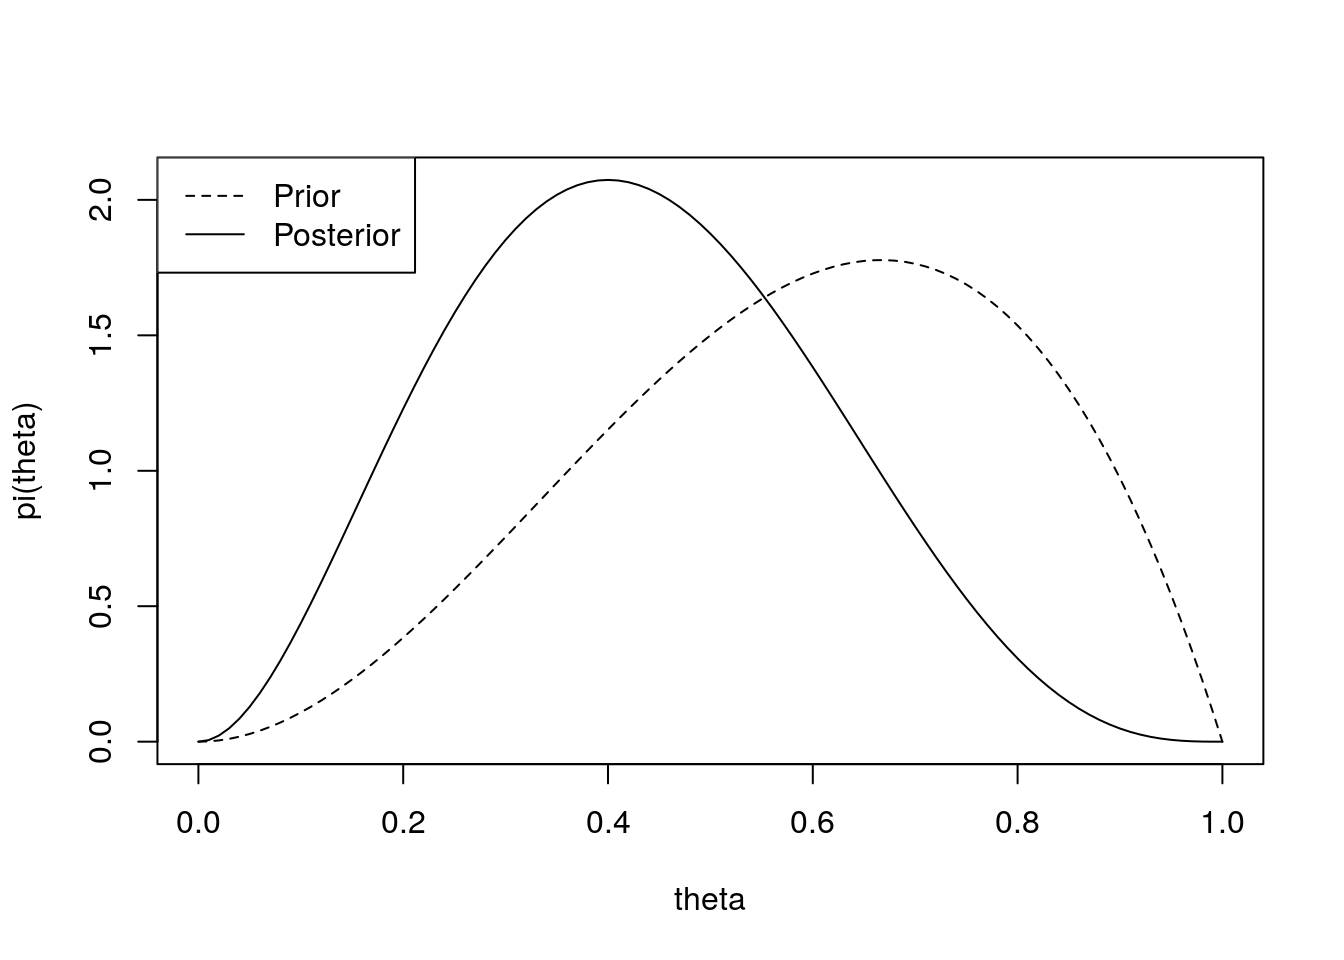
\includegraphics{MATH2011_files/figure-latex/unnamed-chunk-112-1.pdf}

\section{The posterior predictive
distribution}\label{the-posterior-predictive-distribution}

Suppose we wanted to predict the outcome of a new random variables
\(Y_{n+1}\), assumed to have the same distribution as
\(Y_1, \ldots, Y_n\).

If the \(Y_i\) are discrete random variables, the posterior predictive
distribution is
\[P(Y_{n+1} = y | y_1, \ldots, y_n) = \int_\theta p(y; \theta) \pi(\theta | y_1, \ldots, y_n) d \theta. \]

\BeginKnitrBlock{example}[Bernoulli]
\protect\hypertarget{exm:unnamed-chunk-113}{}{\label{exm:unnamed-chunk-113}
\iffalse (Bernoulli) \fi{} }Continuing Example \ref{exm:bayesbern}, with
\(Y_i \sim \text{Bernoulli}(\theta)\) and prior
\(\theta \sim \text{beta}(m_0, n_0)\), recall that
\(\theta|y_1, \ldots, y_n \sim \text{beta}(s + m_0, f + n_0),\) where
\(s = \sum_{i=1}^n y_i\) and \(f = n - \sum_{i=1}^n y_i\). We have
\[\pi(\theta|y_1, \ldots, y_n) = \frac{1}{B(s + m_0, f + n_0)} \theta^{s + m_0 - 1}
(1 - \theta)^{f + n_0 - 1}, \quad 0 < \theta < 1,\] and
\[p(y; \theta) = \theta^y (1 - \theta)^{1 - y}, \quad y \in \{0, 1\}.\]
We have

\begin{align*}
P(Y_{n+1} = 1 | y_1 \ldots y_n) &= \int_0^1 \theta
 \frac{1}{B(s + m_0, f + n_0)} \theta^{s + m_0 - 1}
(1 - \theta)^{f + n_0 - 1} d\theta \\
&= \frac{1}{B(s + m_0, f + n_0)}  \int_0^1 \theta^{s + m_0}
(1 - \theta)^{f + n_0 - 1} d \theta \\
&= \frac{B(s + m_0 + 1, f + n_0)}{B(s + m_0, f + n_0)} 
 \int_0^1 h(\theta) d \theta \\
 & \quad \quad \text{where $h(\theta)$ the $\text{beta}(s + m_0 + 1, f + n_0)$ pdf} \\
&= \frac{\Gamma(s + m_0 + 1) \Gamma(f + n_0)}{\Gamma(s + m_0 + 1 + f + n_0)}
 \cdot
\frac{\Gamma(s + m_0 + f + n_0)}{\Gamma(s + m_0)\Gamma(f + n_0)} \cdot 1 \\
&= \frac{\Gamma(n + m_0 + n_0)}{\Gamma(n + m_0 + n_0 + 1)} 
\frac{\Gamma(s + m_0 + 1)}{\Gamma(s + m_0)}  \\
&= \frac{s+m_0}{n + m_0 + n_0}.
\end{align*}

In our tennis match example, with \(m_0 = 3\), \(n_0 = 2\), after
observing two matches both won by Bob (\(s = 0\), \(f = 2\)), our
predicted probability that Alex will win the next match is
\[P(Y_3 = 1 | y_1, y_2) = \frac{0 + 3}{2 + 3 + 2}= \frac{3}{7}.\]
\EndKnitrBlock{example}


\end{document}
